\part{Methods}
\chapter{Experimental assay, Results~\ref{chapter:p1}}
\chaptermark{Assay v1}
\label{chapter:assay_v1}
\epigraph{Though this be madness, yet there is method in't.}{William Shakespeare\\Hamlet, 1601}
We used monoclonal EL4.NOB1 cell lines that had been gene edited to express fluorescently tagged MyD88 with eGFP and IRAK4 or IRAK1 with mScarlet at the endogenous gene loci. Elke Ziska, Nichanok Auevechanickul and Marcus J. Taylor gene edited cells using CRISPR/Cas9. To separately image MyD88 recruitment, oligomerization and co-assembly with IRAK4/1, I used three clonal lines: (1) EL4.NOB1-MyD88-mEGFP, (2) EL4.NOB1-MyD88-EGFP/IRAK4-mScarlet and (3) EL4.NOB1-MyD88-GFP/IRAK1-mScarlet. The CRISPR/Cas9 endogenous gene tagging approach limits overexpression artifacts. It also allows me to understand the molecular dynamics and discrete intermediate stages of Myddosome formation at physiologically-relevant expression levels.

To validate that gene-edited cell lines expressed the correct protein fusion and that these fusions did not perturb signal transduction, the following controls were performed. Elke Ziska and Nichanok Auevechanickul verified correct insertion of the fluorescent protein in edited genomic loci using sequencing. Elke Ziska confirmed the correct molecular weight of the fusion protein using western blot analysis. Finally, we did several other controls to check that our fusion proteins do not have a perturbed IL-1 signaling transduction.

Numerous reports show that fluorescent protein fusions may perturb signaling functions (Miyawaki, 2003; Haugh, 2012). To ensure this was not the case we performed the following controls. Fenja Gerpott measured IL-2 release using ELISA. EL4.NOB-1 cells are known to secrete IL-2 in response to IL-1. Thus, this provided a bulk assay to determine that IL-1 transcriptional responses were unperturbed by tagging Myddosome proteins.

As a final control, IL-1 stimulated wild-type and gene edited EL4.NOB-1 cells were fixed and stained with antibodies against the RelA subunit of NF-κB and phosphorylated MAPK p38. The nucleus was counter-stained with DAPI. The fixed cells were imaged using a 20\times objective and widefield microscopy (Fig. \ref{p1:S2}), sample preparation and microscopy performed by Fakun Cao).


\begin{centering}
\centering{\includegraphics[width=\textwidth, height=\textheight, keepaspectratio]{jcb/figs2.png}}
\captionsetup{parbox=none}
\captionof{figure}[Gene-edited EL4 cells reconstitute RelA nuclear translocation and MAPK p38 induction.]{\textbf{Gene-edited EL4 cells reconstitute RelA nuclear translocation and MAPK p38 induction.}
\\
\\
(A) RelA translocation to the nucleus in WT and gene-edited EL4 cells. EL4 cell lines (30 min after addition to IL1{\textbeta}-labeled SLBs) were fixed and stained for RelA (magenta); DAPI stained nuclei (blue). Scale bar, 50 µm.
\\
\\
(B) Quantification of RelA nucleus-to-cytoplasm staining ratio. Violin plots show the single-cell distribution RelA nucleus-to-cytoplasm staining ratio. Colored dots superimposed on violin plots correspond to the average value in the independent experiments (n = 3 or 4 experimental replicates per cell line; each replicate encompasses measurements from >2,000 cells. Bars represent mean $\pm$ SEM. P values were calculated using a two-tailed unpaired Student's t test.
\\
\\
(C) Phospho-p38 staining intensity in WT and gene-edited EL4 cells. EL4 cell lines (30 min after addition to IL1{\textbeta}-labeled SLBs) were fixed and stained for phospho-p38 (magenta); DAPI stained nuclei (blue). Scale bar, 50 µm.
\\
\\
(D) Quantification of phospho-p38 staining intensity. Violin plots show the single cell distribution phospho-p38 staining intensity. Colored dots superimposed on violin plots correspond to the average value in the independent experiments (n = 3 or 4 experimental replicates per cell line; each replicate encompasses measurements from >6,000 cells). Bars represent mean $\pm$ SEM. P values were calculated using a two-tailed unpaired Student's t test.
\\
\\
(Images obtained by Fakun Cao. Panels A, C plotted by Fakun Cao. Panels B, D analyzed, plotted by the thesis author. Figure, description extracted from from Deliz-Aguirre et al., 2021.)}
\label{p1:S2}
\end{centering}

Cell culture, gene editing, assays, imaging, data acquisition, statistical analysis, staining, and validation is described in Deliz-Aguirre, et al., 2021 and Cao, et al., 2023. 


\chapter{Stoichiometries from images: Puncta quantified with a custom image analysis pipeline}
\chaptermark{Pipeline v1}
\label{chapter:pipeline_v1}
\epigraph{Science cannot solve the ultimate mystery of nature. And that is because, in the last analysis, we ourselves are a part of the mystery that we are trying to solve.}{Attributed to Max Planck}

To understand how the Myddosome forms, I started by analyzing the dynamics of MyD88-eGFP in cells that had been activated with the aforementioned SLB system (Fig. \ref{p1:1}A, microscopy data generated by Mariam Chupanova, Marcus Taylor and myself).

I observed that after a few minutes of cell contact with the SLB, MyD88-eGFP is recruited to the cell surface and forms puncta (Fig. \ref{p1:3a}A). Initially these MyD88-GFP puncta were dim and transitory (Fig. \ref{p1:3a}). Over time, I observed that brighter and stable puncta formed (Fig. \ref{p1:3a}).

Previous imaging experiments had shown that these MyD88-GFP puncta colocalized with fluorescently labeled IL-1 tethered to the SLB (data acquired by Marcus Taylor) (Fig. \ref{p1:1}B). Based on this observation, I hypothesized that a portion of these MyD88-GFP puncta are fully assembled Myddosome complexes, and that smaller, dimmer and transitory puncta represent the nucleation and oligomerization of MyD88—the initial stage of Myddosome formation.

The existence of intermediary steps in Myddosome assembly is unknown. To understand and quantify these intermediary steps, I developed an analysis pipeline that used particle tracking to identify MyD88-GFP puncta within the high spatiotemporal resolution imaging of live cells.

We took images using a sCMOS camera. To remove the camera's dark-current noise, we captured over a thousand images with the shutter closed at the same exposure as the experimental images. Then, we subtracted the average of these thousand frames from the experimental images.

To minimize the contribution of background fluorescence intensity to measurements of puncta intensity, I passed TIRF-M images through a median filter to estimate background fluorescent intensity across the entire image. This estimated background was subtracted from the image.

Using particle tracking (Tinevez et al., 2017), I extracted the fluorescence intensity of MyD88-GFP puncta. The resulting brightness measurements would be in arbitrary units, and offer no stoichiometric insights. Stoichiometric measurements would allow us to compare our live cells to the stoichiometry (oligomer length) of purified Myddosomes (Lin et al., 2010).

I calibrated the TIRF-M fluorescence measurements with single fluorophores of GFP. This allows me to normalize the signal. It offers insights into the stoichiometry of individual MyD88 puncta. It also allows me to compare the images captured on different dates. Now, we have a system which lets me estimate MyD88 copy numbers from individual puncta. I can finally compare the fluorescent measurements to the biochemically-determined stoichiometries (Lin et al., 2010).

This image analysis pipeline also allowed me to assay the kinetics of MyD88 assembly and quantitatively identify intermediate stages of Myddosome assembly (full detail of image analysis pipeline see Methods, “Image analysis pipeline v.1”).


\begin{centering}
\centering{\includegraphics[width=\textwidth, height=\textheight, keepaspectratio]{jcb/Workflow.png}}

\captionsetup{parbox=none}
\captionof{figure}[short caption]{\textbf{Pipeline workflow.}
\\
\\
(1) Images are converted to TIFF. The background is removed.
\\
\\
(2) Images are segmented using the MyD88 channel.
\\
\\
(3) Cells are cut out of the original image and made into substacks. Then, puncta are tracked with TrackMate.
\\
\\
(4) Intensities are extracted with MATLAB.
\\
\\
(5) The MATLAB tables are converted to CSV and in a style which R can read.
\\
\\
(6) The area and background intensity of cells measured by ImageJ are combined into one table.
\\
\\
(7) The puncta are colocalized using a MATLAB script.
\\
\\
(8) The data is analyzed and plots are made using the aforementioned tables.}
\label{fig:p1M}
\end{centering}

\section{Pipeline for analyzing the protein dynamics images}
\sectionmark{Dynamics Pipeline v1}
Results~\ref{chapter:p2} uses the “Dynamics Analysis Pipeline. Its scripts and guides are available at \url{https://github.com/MJ-Taylor-Lab/myddosome-dynamics-pipeline}. The description is available at Deliz-Aguirre et al., 2021.

The pipeline has eight steps:
\begin{enumerate}

\item \textbf{01\_TIFF-Subtract.ijm}. Runs on ImageJ.

\begin{itemize}

\item TIFF is the gold standard scientific image format. Our microscope produces proprietary ND2 files which includes a TIFF image plus metadata. This script first splits the 16-bit TIFF stack and metadata from the ND2 files. It then splits channels into different TIFF files. This script is also used to remove the background intensity emanating from dark-frame noise, and the non-specific cytosolic fluorescence. 

\item The camera generates noise from a variety of sources that include dark current, read noise, and thermal noise, as well as photon based response noise like the gain and the flatfield (Diekmann et al., 2022). To correct for the dark current noise and the fixed pattern noise, we generated a dark-frame of the camera noise. This frame is generated first by closing the camera shutter and acquiring several (5000 in our case) frames at the same exposure as the experimental images. Then, these frames are averaged; we used the mean. Lastly, this average image is subtracted from the “experimental” and “calibration” images.

\item Cells have autofluorescence, and this could impact our measurements. The non-specific cytosolic fluorescence was estimated using a median filter. Median filters are edge preserving, thus the estimate will be symmetric to the cell, retaining the proportions seen. The background was calculated for a 25-px (approximately 3.67 µm) radius. This number should roughly correspond to the cell radius.

\end{itemize}

\item \textbf{02\_Segmentation.ijm}. Runs on ImageJ. We segmented the image so that we have biological replicate measurements within an image. This script segments cells using a marker-controlled watershed segmentation (available as a plugin called MorphoLibJ, Legland et al., 2016). The marker controlled watershed segmentation 
This script uses a maximum projection of the channel of the reference protein as the marker. It blurs and dilates the image to capture both the marker and mask.

\item \textbf{03\_Substacks-TrackMate.ijm}. Runs on ImageJ. 

\begin{itemize}

\item To accelerate the cell analysis, we made substacks from the segmented cells. We already had two stacks, a dark-frame stack for tracking puncta, and a median subtracted substack for obtaining the intensities.

\item From the segmented cells, we calculated the area and brightness.

\item The last step was to track the puncta on the dark-frame subtracted image substacks. We used the TrackMate plugin (Tinevez et al., 2017).

\end{itemize}

\item \textbf{04\_Reextracintensities/ReextractIntensities\_04.m}. Runs on MATLAB using a modified script adapted from Taylor et al., 2017. We now have the puncta coordinates, but not the fluorescent intensities. To extract the intensities from the median image, we first extracted the TrackMate coordinates from its XML file output. Then, we segmented a 3\times3 pixel box with sub-pixel localization. Lastly, we extracted the summed intensity from that box and exported it as a table.

\item \textbf{05\_MATLAB-CSV.R}. Runs on R. The MATLAB table was adapted to run on R. with x, y, t, intensity and track ID columns.

\item \textbf{06\_Area-Background.R}. Runs on R. To analyze images on R (later described under 08\_Analysis), we made an output list that list cell tables, their paths, area and intensity.

\item \textbf{07\_Colocalization/run\_trackmate\_anaylsis.m}. Runs on MATLAB using a modified script adapted from Taylor et al., 2017 with coding contributions from Alexander Schmidt (Taylor Lab). For the IRAK4/1 images, we took images of the GFP and mScarlet channels. They were tracked, but separately. Because we were interested in the interplay between proteins, we needed to calculate colocalization. We had three criteria: (1) maximum distance cutoff, (2) minimum association time, and (3) minimum dwell time of the puncta. After this, we generated an output table to be later analyzed in R.

\item \textbf{08\_Analysis}. The last step was the analysis and plotting of the data. Several parameters were calculated for each track, including their dwell time, maximum brightness and intensity change from start to max. We also calculated the max size and recruitment time for the colocalized puncta.

\end{enumerate}

\section{Pipeline for analyzing the staining images}
To assay the level of RelA (NF-κB p65 subunit) and p38 MAPK activation in widefield images of fixed cells , I developed an image analysis pipeline. This image analysis pipeline was implemented in FIJI and R. I implemented a threshold-segmentation in FIJI to identify the cytoplasmic and nuclear volume of individual cells. I segmented and identified individual cells using the MyD88-GFP and the RelA/phospho-p38 staining image. To identify the nuclear volumeI segmented DAPI nuclear stain image. The cytoplasmic volume was identified by subtracting the nuclear volume from the cell volume. We then measured the fluorescent intensity of the two segmented cellular areas. Fluorescent intensity values were then analyzed in R. First I normalized the fluorescent intensity values. For RelA I calculated the cytoplasm to nuclear ratio of RelA staining to assay nuclear translocation. For p-p38, I measured the nuclear staining intensity.

This analysis confirmed that gene-edited cells line expressing fluorescent protein fusion of MyD88 and IRAK4/1 can still activate a downstream IL-1 signal transduction. In conclusion, our tagging strategy did not abolish IL-1R signaling response. These cell lines can be used to investigate the dynamics of IL-1 mediated Myddosome signal transduction.

The staining images analysis pipeline is available at \url{https://github.com/MJ-Taylor-Lab/myddosome-dynamics-pipeline/tree/master/StainingAnalysisPipeline}. The description is available at Deliz-Aguirre et al., 2021.

\chapter{Experimental assay, Results~\ref{chapter:p2}}
\chaptermark{Assay v2}
\label{chapter:assay_v2}
\epigraph{The “dream” of every cell is to become two cells}{François Jacob}

To probe the dynamics of these signaling proteins, we used our assay (cell lines, imaging technique) as described before (Results~\ref{chapter:p1}, Deliz-Aguirre et al., 2021), with improvements in the image analysis (Methods~\ref{chapter:PIRATES_PARLEYS}). To compare cell lines and establish a temporal order, proteins were tagged in pairs. Elke Ziska, Fakun Cao, Nichanok Auevechanickul, Claudia Abad-Baucells and Elba del Val Oriza fluorescently labeled the aforementioned proteins at the endogenous loci using CRISPR/Cas9. There was an upstream reference protein, MyD88, tagged with eGFP. The downstream proteins were tagged with mScarlet. Proteins were validated as described before. Then, labeled cells were imaged using TIRF-M. To quantify the dynamics, the images were processed with a pipeline that uses Python, ImageJ and R (Methods~\ref{chapter:PIRATES_PARLEYS}).

\chapter{PIRATES-PARLEYS: A high-throughput image analysis pipeline that quantifies protein dynamics}
\chaptermark{High-throughput pipeline}
\label{chapter:PIRATES_PARLEYS}
\epigraph{Familiar things happen, and mankind does not bother about them. It requires a very unusual mind to undertake the analysis of the obvious.}{Alfred North Whitehead\\(Science and the Modern World, 1925)}

Biochemical characterization of proteins reveal a long list of interactors involved in pathways. However, bulk cell analysis lacks spatiotemporal resolution and cannot solve subcellular protein dynamics. To address this, fluorescent microscopy is used to visualize how individual proteins transduce a cellular signal. My goal was to develop a high-throughput (“supercomputer” compatible) image analysis pipeline for quantifying protein dynamics as seen using live-cell fluorescent microscopy.

Myddosomes form punctate structures that are highly dynamic, growing and shrinking, persisting for varying amounts of time (Deliz-Aguirre et al., 2021). We saw that protein colocalization is equally dynamic, with a wide range of MyD88 oligomer lengths being able to recruit downstream IRAK4 and IRAK1 (Deliz-Aguirre et al., 2021). However, these puncta are diffraction limited. They also split and merge frequently. To understand the dynamics of protein colocalization, I opted for a large sample size (N) approach and quantified thousands of puncta, so that I can measure small differences accurately and precisely. I was interested in studying protein colocalization dynamics because the imaging showed a highly dynamical system. Quantifying biological dynamics could potentially offer clues as to how proteins regulate one another.

I used our live-cell assay as described before (Results~\ref{chapter:p1}); Deliz-Aguirre et al., 2021; Fig. \ref{p1:1}) and revised it (Methods). For Results~\ref{chapter:p2}, proteins were tagged in pairs: an upstream reference protein (MyD88, and TRAF6 in the TRAF6-NEMO cell line) tagged with eGFP, and a query downstream protein tagged with mScarlet. Proteins were validated as described before. Then, I proceeded to quantify the microscopy images with our new pipeline. Here, I will describe a new pipeline called Pipeline for Image analysis with Reference images, Automated Tracking, Extraction of intensities, and Segmentation (PIRATES) Phase portrait Analysis and Relative kinetics comparison Localization analysis with Extraction of data Yielding Statistics (PARLEYS), and why it was needed.

Our first pipeline was able to quantify the microscope images, tracking puncta over time and measuring their intensities. However, the previous pipeline had a few drawbacks which we have now addressed and will be discussed below. Additionally, new techniques have been incorporated. Briefly, this new pipeline is able to run considerably faster, it requires less user involvement, and it simplifies the measuring of colocalization using a soft matter physics approach.

\section{Steps}
\subsection{Dark-current noise was subtracted with minimal user input}
\subsectionmark{Dark-frame}
Starting with the image acquisition, there are several camera sensor types available in the market. The most popular scientific camera sensors are charge-coupled devices (CCDs) and scientific complementary metal-oxide-semiconductor (sCMOS). CCD sensors capture less noise and are highly sensitive (they have high quantum efficiencies). However, they are slow in capturing images. By comparison, sCMOS sensors are fast, and are making leaps in quantum efficiencies nearing CCD sensors. To capture our dynamic fluorescent proteins, we opted for the fast sCMOS sensor.

Camera sensors work by converting photons into electrons. The proportion that gets successfully converted is called the quantum efficiency, which nowadays hovers around 90\%. Then, these electrons are read and converted into a number. One issue with sCMOS sensors is that they are noisy, that is, the signal fluctuates randomly. 

As with other sensitive camera sensors, one source of noise for sCMOS sensors is the dark-current, that is, thermal noise, the heat from the camera. We used liquid cooling to lower the sensor temperature down to -20ºC (253.15 K), and keep it stable (unstable temperatures can potentially produce thermal expansion whose deformations would produce shape aberrations). However, this is not enough to completely remove thermal electrons, which theoretically would need the temperature to be absolute zero (0 K) in order to have no noise. I used image processing to remove the dark-current noise.

This camera noise can be estimated by averaging several pictures with the camera shutter closed (Fig. \ref{m:1}.1). The more frames, the better, though there will be a point where capturing more images will not change the average. In my case, I overshot and took over a thousand images with the shutter closed (already at around 100 frames and 50 ms exposure, the average stabilizes), and then mean-averaged these frames (Fig. \ref{m:1}.1). The resulting single image is called the dark-frame (Fig. \ref{m:S1}.4 Dark-Frame).

The dark-frame exposure should be the same (or near) the experimental image exposure. This is because the higher the exposure, the higher the dark-frame intensities are because the sensor has more time to accumulate thermal electrons.

Now that I have calculated the dark-frame, and captured experimental images, I have to tell the computer which images to analyze and how. All the parameters needed to run all scripts are given by the user at this point. This is done in a single step using csv tables (Fig. \ref{m:1}.2; Methods). It is an improvement from the previous pipeline in that the previous pipeline had eight steps that required the user to input data. Now, everything runs in a single step.

The first step the pipeline makes is converting images into standard image formats. Each pixel is an xy-coordinate, thus the fluorophore brightness detected by the camera sensor (the intensity) is saved as a matrix, typically into a tag image file format (TIFF) file. TIFF is the gold-standard scientific image format. However, our Nikon microscope produces proprietary ND2 files which includes a TIFF image stack plus metadata. To enable image processing, the pipeline first extracts the 16-bit TIFF image stack (frames set, the “video”) and metadata from the ND2 files (Fig. \ref{m:1}.3). One drawback of the previous pipeline was that it required heavy user involvement at every single step of the way. With my new pipeline, the scripts use the image metadata to make decisions (Fig. \ref{m:1}.3). 

The next step is removing the dark-frame. The previous pipeline removed the dark-frame from the experimental images. However now, the script automatically selects the appropriate dark-frame image. It identifies which dark-frame exposure is closest to that of the experiment. \begin{equation}\text{dark-frame}_{\text{exposure}} = min(|\text{image}_\text{ exposure} - \text{dark-frame}_{\text{exposure}}|)\end{equation} After, the pipeline subtracts the dark-frame from the experimental images (Fig. \ref{m:S1}.4; \ref{m:1}.4). The resulting image has less background noise. \begin{equation}\text{image} = \text{image} - \text{image}_\text{dark-frame}\end{equation}

\begin{centering}
\centering{\includegraphics[width=\textwidth, height=\textheight, keepaspectratio]{methods/figS1.png}}
\captionsetup{parbox=none}
\captionof{figure}[Subtracting the dark-frame removes the background noise]{\textbf{Subtracting the dark-frame removes the background noise.} For visualization purposes, I cropped a cell out of the original image so that detail can be appreciated. This cropped box measures 17.31 µm by 16.43 µm (0.1467 µm/pixel). Also for illustrative purposes, the contrast is rescaled each time using the auto-contrast function of ImageJ. While images are monochromatic, I used the viridis plasma look-up-table (LUT) because this color map offers higher visual contrast while being colorblind friendly. Then, I inverted the LUT so that the colors can be appreciated in print media. Back to the dark-frame subtraction, I first estimated the camera dark-frame, that is, the thermal noise. To estimate such noise, I captured 1000 images at the same exposure as the experimental image, but with the camera shutter closed. That way, only camera noise is captured in the images. The correct exposure time is important because the longer the acquisition, the more thermal electrons are accumulated, which translates into thermal noise. This dark-frame was subtracted from the original image.}
\label{m:S1}
\end{centering}

\subsection{Different images for different purposes: the tracking and intensity images}
\subsectionmark{Tracking, intensity mages}
My objective was to track protein puncta (spots) over time and measure their intensities. To see the protein dynamics, proteins were labeled with fluorophores, so that the proteins of interest can be selectively visualized. Thus, we used fluorescence microscopy to visualize live-cell protein dynamics. Quantitative fluorescent microscopy works by measuring light apart from the background.

To track the proteins, I need images that are excellent for tracking which must have high signal-to-noise ratios (bright puncta and dark background) for reasons that will be discussed later in this section.
\begin{equation}
\text{SNR} = \frac{\text{signal}}{\text{noise}} = \frac{\mu_{int\text{ puncta}}}{\mu_{int \text{ background}}}
\end{equation} 
Where $SNR$ is signal-to-noise ratio, $\mu$ is the mean, and $int$ is intensity.
The signal-to-noise ratio is a metric of how good the contrast is in an image. In my case, the signal is the brightness of the fluorophore and the background is the rest. A high signal-to-noise ratio is desirable, and there are several ways to achieve this. It can be classified as before, during or after image acquisition. Each method has its own advantages and drawbacks, but they can be combined to get a better quantifiable image, which is what this pipeline does.

Before image acquisition, one can use bright fluorophores to produce a better signal. However, there are several considerations when using fluorescent proteins. Fluorescent proteins can produce steric hindrance which would disable complexes from forming properly. In addition to trying different molecules, one way to bypass hindrance is to tag either the C or the N terminal of the protein. The fluorescent protein needs time to maturate. Therefore, experimenters need to be aware of when a protein can be visualized. Another fluorophore consideration is that when attempting multi-color imaging, the selected fluorophore emissions (light wavelength color that bounces back) should not be near (Fig. \ref{m:S2}5). Outside fluorescent proteins, there are fluorescent organic dyes, and while they can be brighter than fluorescent proteins, dyes need to be conjugated. For my experiments, we used eGFP and mScarlet.

Another approach to improve the signal before image acquisition would be to use more laser light. This would be at the expense of photobleaching (fluorophore no longer emitting light) and phototoxicity (photons damaging molecules inside cells). In my case, I opted for low laser light to reduce photobleaching, so that I can collect more timepoints.

For decades, TIRF microscopy has been used to improve the signal-to-noise ratio before image acquisition. TIRF microscopy works by selectively illuminating the surface next to the coverslip in what is called the evanescent field. For visible light, this is around 100 nm. Fluorophores outside this field cannot be excited which means it cannot emit light. This makes TIRF excellent at reducing the background fluorescence dramatically. It also means that theoretically, fluorophores will not be exposed to light, which means the effects of photobleaching are reduced. However, for some applications, TIRF microscopy is not feasible as it cannot visualize structures more than 100 nm which is a fraction of the size of many eukaryotic cells (humans, mice, yeast). Because I wanted to visualize protein dynamics of receptor signaling, I used TIRF microscopy.

Then during image acquisition, one can use a higher exposure. This is beneficial because fluorophores blink (turn on and off, vs photobleaching which is permanently off). Meaning, low exposures could produce gaps in visualization. Another benefit of the high-exposure approach to reducing noise is that image acquisition is a choreography of hardware. The microscope switches the light filter. The laser turns on. The shutter opens. The camera collects photons. The shutter closes. The process repeats. To address the delays in image acquisition, a setup called triggered acquisition can be used. Instead of the different components (e.g., laser illumination, shutter opening, filter changes) making decisions of when to act, an external machine tells the components when to perform their task. It is for these delays in sending signal that for the same recorded intensity, low-laser high-exposure tends to produce less photobleaching than a high-laser low-exposure setting. However, high exposure has its disadvantages. If the dynamics are faster than the exposure, then there will be gaps in the protein visualization. There is also the potential to introduce motion blur with a high exposure. For my setup, I opted for low-laser high-exposure.

I added a four second delay between the imaging frames acquired because capturing images continuously would result in photobleaching, before the assembly and disassembly of the signaling pathway can be observed

For this assay, assembly is inducible. To control activation of the receptor, I used a supported lipid bilayer (SLB) functionalized with ligand. One way which could potentially control the speed of assembly and disassembly lies on the density of the ligand on top of the glass. We used 32 molecules µm\textsuperscript{-2} to activate cells. This is slow enough to observe the growth, but fast enough to be imaged in 30 minutes.

Post-acquisition, image processing can be used to improve the signal-to-noise ratio. My computational method offers high signal-to-noise, but its drawback is that the intensities become far removed from the original intensities. To counteract this, I generated two image sets: one for tracking and another for measuring intensities (Fig. \ref{m:1}.5). This way, I have images that are optimized for their purpose—the best of both worlds. The tracking image had more processing done, and focused on obtaining the best signal-to-noise ratio. The fluorescent intensity measurement image is less processed, so that the fluorescent intensities are close to the original values as captured by the microscope camera. More on this in the following subsections. For simplicity, I will call these the tracking image and the intensity (reference) image (Fig. \ref{m:1}.5).


\begin{centering}
\centering{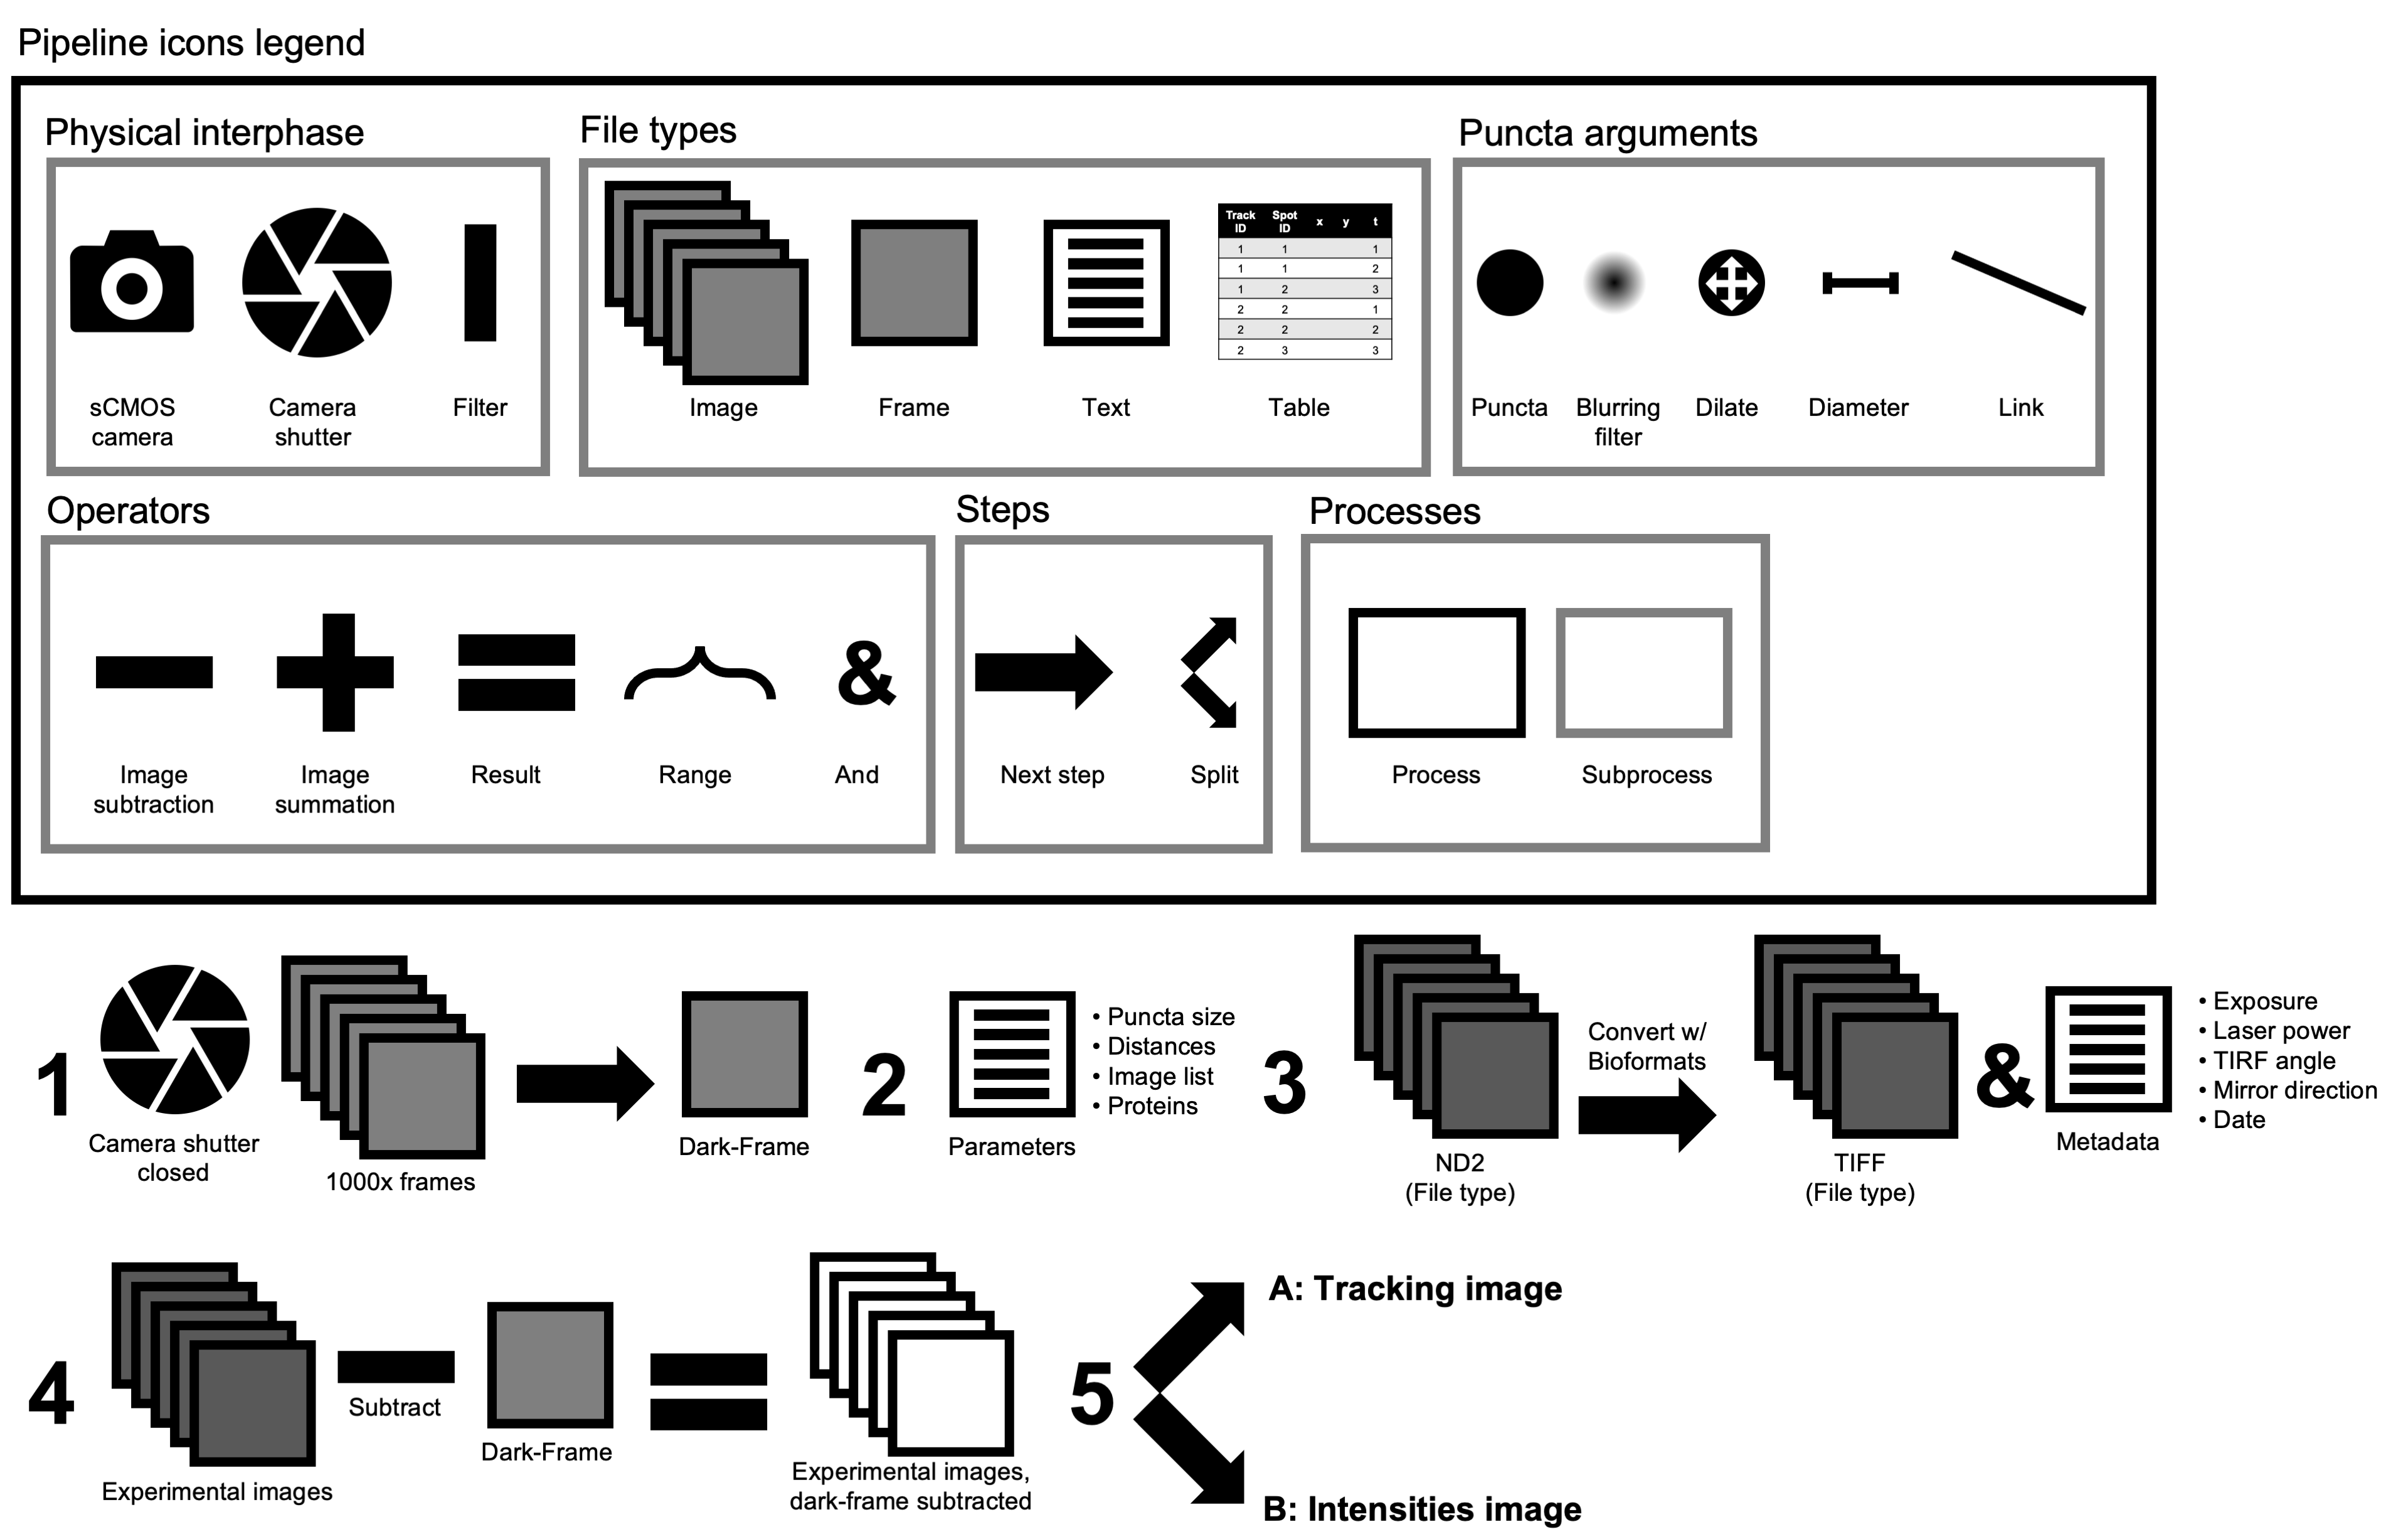
\includegraphics[width=\textwidth, height=\textheight, keepaspectratio]{methods/fig1.png}}
\captionof{figure}[Pipeline uses the metadata to remove the dark-frame]{\textbf{Pipeline uses the metadata to remove the dark-frame.} All icons used in this section are included in the pipeline legend.
\\
\\
(1) The pipeline starts with the determination of the dark-frame, which is the thermal noise in the camera. To calculate the dark-frame, the camera shutter is closed. Then, 1000 frames are acquired at the exposures used in the experiments.
\\
\\
(2) Input the parameters of the pipeline, including the image list, names of proteins in each channel, and the puncta size.
\\
\\
(3) The pipeline starts by converting proprietary formats to TIFF, the gold standard scientific image type. The pipeline saves the metadata. It then extracts useful image information that is needed for future steps. That is, it extracts input parameters so that the pipeline is autonomous, and the user does not have to interact with the pipeline.
\\
\\
(4) The dark-frame is subtracted from the experimental images. The pipeline used the image metadata to make the decision of which dark-frame to use.
\\
\\
(5) The pipeline splits into two processes: calculating the tracking image and the intensities image.}
\label{m:1}
\end{centering}

\subsection{The tracking image uses median subtraction, median blur and moving averages}
\subsectionmark{Tracking image}
To obtain the sharpest puncta, I estimated the background around the puncta (emerging, for example, from diffused light) using a median filter (Fig. \ref{m:2}.5A). Median filters are a type of smoothing filter whose strength is edge preservation. Edge preservation is the ability to remove (blur out) noise while keeping a sharp edge, that is, keeping the silhouette. This contrasts with Gaussian filtering in that Gaussians blow-up the image features (in computer vision, features are information of image properties). For estimating the background around a puncta, I used a slightly dilated diameter from the puncta diameter used in particle tracking. I duplicated the puncta size. This would result in a 10-pixel diameter. Median filters extract all the values around a defined circle diameter, and sorts the values from smallest to largest, and then assigns the middle value to the center of the circle. The equation of a median is:
\begin{equation}
\text{Median}(X) = 
\left\{\begin{array}{lr}
X[\frac{n+1}{2}], & \text{if }n \text{ is odd}\\
\frac{X[\frac{n}{2}]+X[\frac{n}{2}+1]}{2},& \text{if }n \text{ is even}
\end{array}\right.
\end{equation} where $X$ is an ordered list of intensities and $n$ is the diameter of the median filter. If I use a 10-pixel size diameter ($n$), then there would be two middle values which are then settled by calculating the mean of the two center values. In other words, I would calculate the mean ($\mu$) for the two middle values ($n/2$ and $n/2+1$). This is an issue because if the data is non-parametric (for example, log distributed), then the mean ($\mu$) will be skewed. To employ a true median ($\frac{n+1}{2}$), I used a 11-pixel radius for estimating the background around a puncta (Fig. \ref{m:2}.5A). The middle value would then be the 6th pixel intensity in the ranking. Lastly, I subtracted the median-blur image from the experimental images whose dark-frame was subtracted (Fig. \ref{m:2}.5A). Calculating medians is computationally intensive which is why it is not employed as frequently as Gaussian blurs. It has to rank all pixels instead of summing them. There is a need to increase the speed of processing.

My previous pipeline did not make use of the full computing power available, running single-threaded in one central processing unit (CPU) only. For this second pipeline, I parallelized the scripts to make use of all the computer CPU resources available. Parallelization is a process which breaks tasks into smaller tasks and distributes them across processors. This approach enables using multiple processors for the job, and speeds up the analysis considerably as a result. More importantly, the scripts were rewritten so that it is compatible with cluster computers (supercomputers). For the cluster I used, Raven of the Max Planck Computing and Data Facility (Garching, Bavaria, Germany), I had 72 CPUs available. Theoretically, this means scripts now run 72\times faster. In principle, it could run faster using graphical processing units (GPUs), but this requires specific hardware which would make my scripts less accessible to the scientific community at large.

The camera generates random fluctuations for each pixel, independent of the puncta fluorescence intensities (Diekmann et al., 2022). I used two methods to address this which can be thought of as time-independent and time-dependent in that the time independent uses only one frame and the time-dependent takes multiple observations taken at multiple times. Starting with the time-independent method, I applied a median blur of 3-pixels to even out the field (Fig. \ref{m:2}.5A). Because puncta are 5-pixels in diameter and median filters are edge-preserving (keeps silhouette), a 3-pixel median-blur would still be able to show punctate structures while removing noise. However, the intensity measurements are now skewed, and random noise can appear punctate-like. To counteract this, I obtained intensity measurements from another image.

The second method for (“time-dependent”) random interference noise reduction that I used is called the moving average. In addition to counteracting random fluctuations emanating from the camera sensor, moving averages also help account for fluorophores blinking (flicker) (Dickson et al., 1997).

Moving average projections (image combination) work first by splitting the image into subsets of frames (k, also called the window) (Fig. \ref{m:2}.5A). It then calculates the average of each pixel intensity at the same xy coordinate, and after, it creates a new list of average values which uses the xy coordinates to become an image. The frame is then shifted by one and the process is repeated again, that is, take the preceding and succeeding (original) frame, and calculate the mean. The other way to do this is a more familiar method which is called a group t-projection (group time combination). Group projection would average the three frames, and move three frames forward, and repeat the process again. The running average produces the same number of frames minus the window plus one while the group t-projection would divide the number of frames by the window size. For our window of three frames, say I have 99 frames in the original image, the running average that I use would produce 97 frames while the group t-projection would offer 33 frames. It is for this reason that I use the running average method.
\begin{equation}
\text{SMA}_k = \frac{int_1 + int_2 + \cdots + int_k}{k}
\end{equation}
Where $k$ is the window.

Running averages can potentially create an artifact known as motion blur (ghost-like image trails) which is an undesired consequence of the camera exposure. This effect emerges because camera exposure needs to be high enough to capture light, but not too high as to make it impossible to identify puncta. Motion blur arises in puncta that are traveling fast. For a single frame, this can be calculated as half the pixel length per exposure time.
\begin{equation}
blur_{\text{tolerance}} = \frac{\text{pixel size}}{2}\times \text{exposure}
\end{equation}

Our camera has a resolution of 0.147 µm/pixel, thus motion blur would emerge for puncta traveling faster than 0.37µm/s for a 200 ms exposure, or 1.46 µm/s for a 50 ms exposure. This is the tolerance (parametric limit) for the intensity reference image. However, because we are using a running average with a window of three frames (or 12 seconds since we use 0.25 frames per second), our objects would need to move between 0.03 to 0.12 µm/s for exposures at 50 and 200 ms, respectively, to be tracked appropriately.
\begin{equation}
blur_{\text{tolerance}} = (\frac{\text{pixel size}}{2}\times \text{exposure}) \times (k \times \text{frame rate})
\end{equation}
where $k$ is the window.

The easiest way to offset the effects of motion blur would be to use a responsible small window, which in my case, I used three frames (it is an odd number so that values can be centered; say we have three frames, it would use the time of the second frame as the new timestamp) (Fig. \ref{m:2}.5A).

Motion blur can create long tails that seem like comets. Another way to remove the effects of motion blur lies in the rigid 5-pixel diameter of the puncta that TrackMate uses in detection. TrackMate detects puncta by fitting 2D-Gaussian curves (normal curves in xy axis) (Fig. \ref{m:4}.7A), then calculates the derivative (change between pixel before and after) of the fit, and after, applies a Laplacian operator (second derivative, that is, the change of change) to find edges (boundaries). The result is then inverted, and TrackMate then centers the puncta around the local maxima (relative brightest value) (Fig. \ref{m:4}.7A). Thus in a perfect world, an image moving linearly whose intensity remains constant would have the correct puncta centroid. However, puncta moving randomly (like Brownian motion) would have a less accurate centroid. For my system, MyD88 is likely traveling via the cytoskeleton, which means movement is predictable. However, if the intensity fluctuates, TrackMate could potentially use the wrong centroid. This is another reason why I use the intensity reference image, to counteract this.

Another artifact motion blur can introduce is overcorrection. Puncta that persist only for one frame would be dimmer than the original intensity (if using the mean as it would average two dim values and one bright value), or disappear (if using median as the center value of two dim and one bright event would be a dim event). However, distinguishing noise from puncta would be difficult, and our script requires a minimum dwell time (persistence) of three frames in order for puncta to be included in the analysis. Another artifact that could be introduced is having “shadow” intensities in the preceding and succeeding frames. While this can be an artifact, it can also be advantageous in that it can boost intensities of dim puncta, and allows us to measure the beginning and the end of the puncta better. Moreover, we obtain intensities from a different picture. At worst, the intensity would read close to zero, which means it can be addressed in the post-processing of the images as I have an intensity reference image.


\begin{centering}
\centering{\includegraphics[width=\textwidth, height=\textheight, keepaspectratio]{methods/figS2.png}}
\captionof{figure}[The tracking image offers high signal-to-noise at the expense of skewing intensities]{\textbf{The tracking image offers high signal-to-noise at the expense of intensities.} The tracking image is highly processed so that high signal low background can be achieved. However, this comes at the expense of the intensity values which are now considerably lower than the dark-frame removed image. The tracking image starts with the estimation of the background around the puncta using a median (edge-preserving) filter of size 11-pixels (2\times puncta size + 1 to make it odd, that is, a true median). Then, the blur is subtracted from the dark-frame removed image. This results in an image with low cytosol noise. Yet, there is considerable noise due to random intensity fluctuations. To remove this source of noise, I took two approaches, one time independent and another time dependent. The time independent method uses median blurs of a diameter slightly smaller than the puncta. In this case, it is 3-pixels. The resulting blurred image is then passed through a moving average filter, so that random fluctuations can be removed in a time dependent manner. I took three frames, and averaged the intensities, pixel by pixel (xy coordinate). Then, the resulting mean image is saved. This process is done iteratively, shifting by one frame. The resulting image is then summed with all other channels (the reference plus the query proteins). The output of this I call the tracking image.}
\label{m:S2}
\end{centering}
 
\begin{equation}
\text{tracking image = }\sum_{i = 1}^{c}\text{dark-frame removed image}_i
\end{equation}

Proteins are labeled with fluorophores so that they can be selectively visualized with fluorescence microscopy. This is the principle of fluorescence microscopy. For fluorophores to be seen, they need to be excited (illuminated) with a particular wavelength (Fig. \ref{m:2}.5). Then, they emit (bounce) at another specific wavelength (Fig. \ref{m:2}.5). In the case of green fluorescent protein (GFP), the excitation is cyan light and the emission is green light (Fig. \ref{m:2}.5). Cells can reflect the excitation light. To only see the light in the expected emission spectrum, a filter is used to block the excitation light out and let the emission light pass (Fig. \ref{m:2}.5). My camera is monochromatic. This means I can use a single camera to visualize two fluorophores to see two proteins.

To see the different proteins we labeled, we had to capture two images, one at each color channel (eGFP, mScarlet) (Fig. \ref{m:2}.5). I observed punctate structures. Software can track puncta over time. To be able to determine if the different proteins are colocalized, there are two approaches to calculate puncta colocalization: tracking puncta separately or together.

In the previous chapter, I used to track puncta in different channels separately. I used a script to pair puncta in different channels using the distance from its coordinates, and measured how long did these puncta in different channels (proteins) dwell together (called the dwell time). From this, the script then decided which puncta belong together. One issue I had was that it became difficult to distinguish which puncta belongs to who. The cells had several puncta. This meant that sometimes, the script assigned one “reference” protein to several “query” proteins. To make things harder, Myddosome puncta are highly dynamic, continuously splitting and merging. This means a puncta can start with one query puncta that then splits off (completely or partially, both are possible), or puncta merge. To address this issue, the new pipeline combines the different channel images into one (Fig. \ref{m:2}.5A). Now, the decision of which puncta are colocalized rests on the particle tracking software that I used, TrackMate.

With all this in mind, I have now created a tracking image for TrackMate. Later, I will need to fix the timestamp so that it uses the center frame value (Fig. \ref{m:S2}.5A).

\subsection{The intensity image uses median subtraction to remove cytosolic background}
\subsectionmark{Intensity image}
For the intensity image, I first used the dark-frame subtracted images. Then, I median-blurred these images using a 3.7 µm (25-pixel) diameter, about half the cell diameter (Fig. Fig. \ref{m:S3}.5B, \ref{m:2}.5B). The resulting image is an estimate of the cytosol fluorescence (background). After, I subtracted the median blur from the dark-frame removed images (Fig. Fig. \ref{m:S3}.5B, \ref{m:2}.5B). The resulting image is the intensities reference image (Fig. \ref{m:2}.5B). This image will be used to obtain intensity measurements from the puncta (Fig. \ref{m:S3}.5B).

Up to this point, the pipeline has saved four images: the original image, the dark-frame removed image, the tracking image, and the intensities reference image. To calculate the signal-to-noise ratio, I took a sample puncta of 5-pixels in diameter as a signal measurement, and a box outside the cell for my background measurement. From these regions, I calculated the mean intensity and then divided the signal by the background to obtain the signal-to-noise ratio (SNR). The original image had a lot of background. The SNR was two. The dark-frame removed image had most of the camera background eliminated, and had a SNR of seven. After, the intensities reference image whose cytosolic estimate was removed, had a SNR of 31. Lastly, the tracking image had the best SNR, at 40. However, the signal was 73\% dimmer than the dark-frame removed image (Fig. \ref{m:S3}.SN). By comparison, the intensities reference image was 35\% dimmer than the dark-frame removed signal.


\begin{centering}
\centering{\includegraphics[width=\textwidth, height=\textheight, keepaspectratio]{methods/figS3.png}}
\captionof{figure}[Another image set is generated with intensities preserved but cytosol fluorescence removed]{\textbf{Another image set is generated with intensities preserved but cytosol fluorescence removed.} Different images were created with different purposes.
\\
\\
(5B) The intensity reference image is generated so that we have accurate intensity readings. To accomplish this, I first estimate the cytosolic background using a median blur whose diameter is half of that of a cell, about 25-pixels. Then, this background estimate is subtracted from the dark-frame removed image. The resulting image is the intensity reference image. (Signal-to-Noise) To illustrate the advantages of my pipeline, I took a sample puncta and calculated its mean brightness (signal) and then divided it by a region with no cells (the background). The quotient is called the signal-to-noise ratio (SNR). The original image has poor SNR. After removing the dark-frame, there is improvement, but the true improvement happens after processing the image. The intensities reference image has a SNR of 31 which also preserves the signal strength. The tracking image has a SNR of 40 which is great for tracking, but not for measuring intensities. It is for this reason that multiple images were created by this pipeline.}
\label{m:S3}
\end{centering}


\begin{centering}
\centering{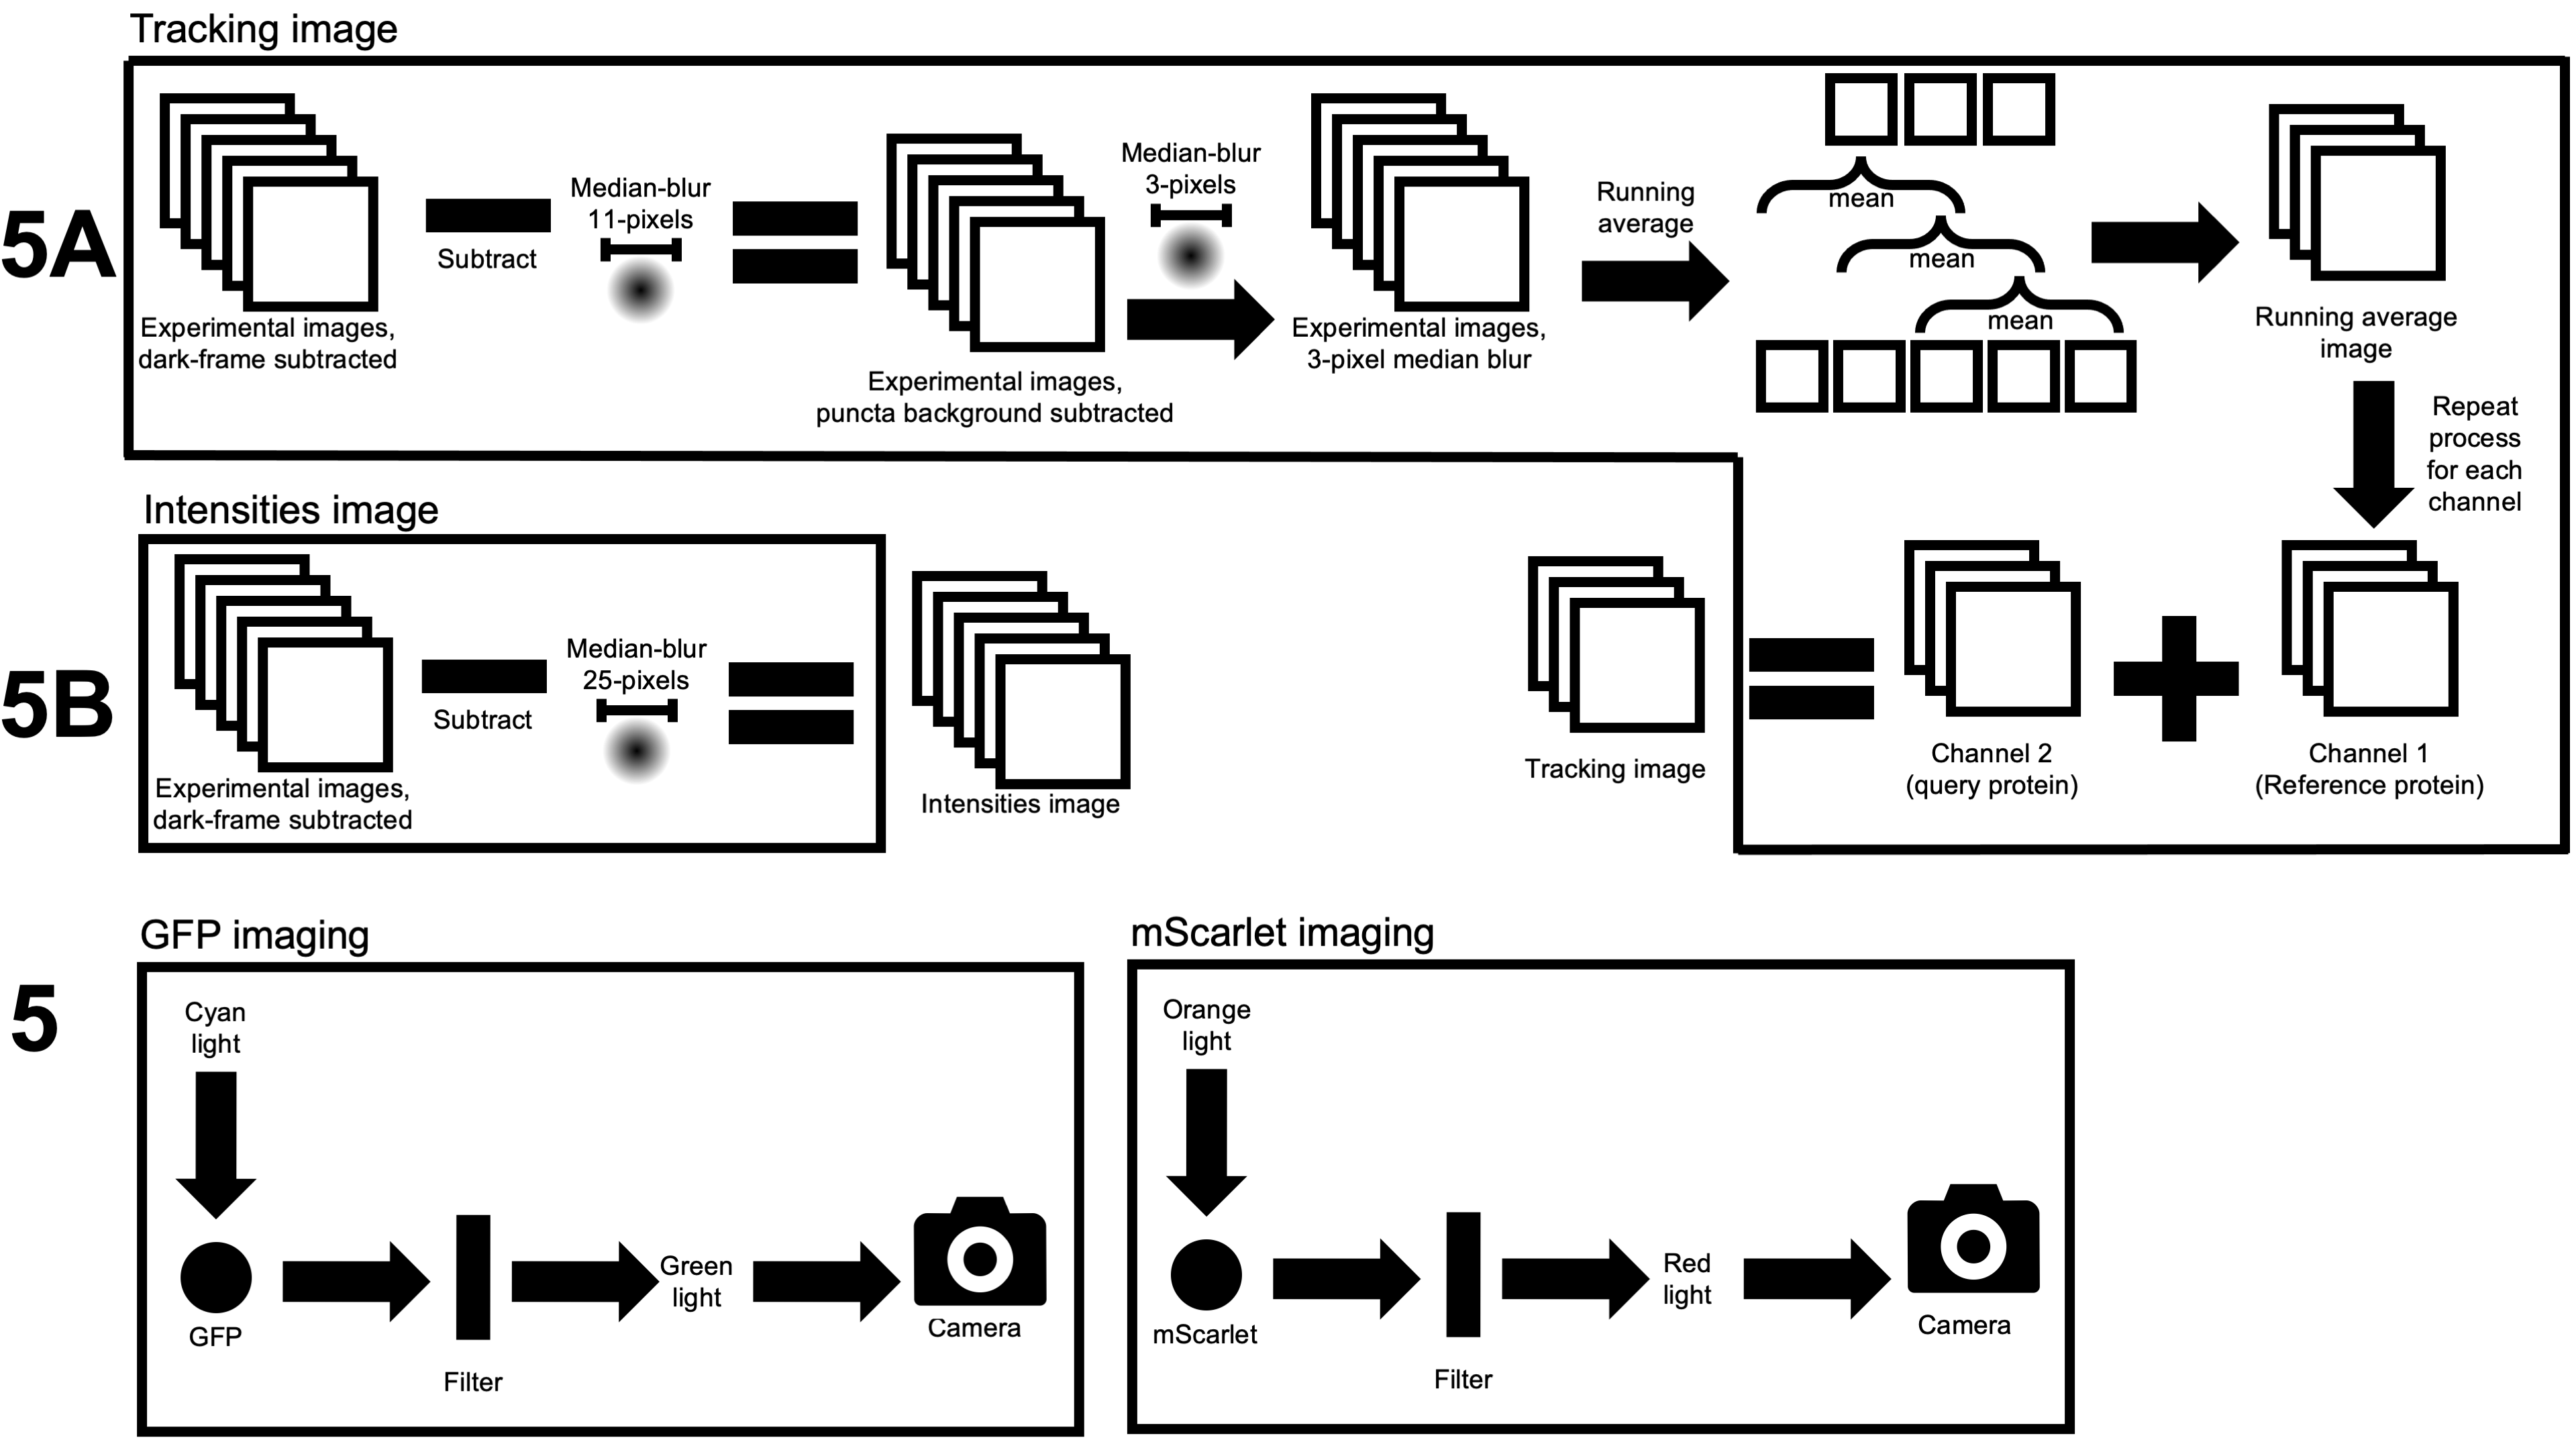
\includegraphics[width=\textwidth, height=\textheight, keepaspectratio]{methods/fig2.png}}
\captionof{figure}[The tracking and intensity-measurement images are created fit for their purpose]{\textbf{The tracking and intensity-measurement images are created fit for their purpose.}
\\
\\
(5A) The tracking image process begins with the subtraction of the puncta background. This is accomplished by calculating a median blur twice as large as the puncta (plus one if this number is even, so that it uses a true median and not an average). Then, it subtracts the blurred image from the experimental image. After, a median blur of 3-pixels in diameter (slightly smaller than the puncta) is applied so that random fluctuations of the camera sensor are removed. Lastly, also for removing random fluctuations, a running average is calculated.
\\
\\
(5B) The intensity-measurement image estimates the cell cytosolic background using half of the cell diameter, that is, 25-pixel in diameter. It then subtracts this blur from the dark-frame removed experimental image.
\\
\\
(5) Diagram showing the microscope setup. Fluorophores are excited with laser light, then a filter blocks out unwanted light that falls outside the expected color. Lastly, the expected light is collected by the sCMOS camera sensor.}
\label{m:2}
\end{centering}


\subsection{Cell segmentation speeds-up the analysis, and enables identifying biological replicates}
\subsectionmark{Segmentation}
The images we captured can potentially fit well over forty cells. If I quantify whole images as-is, then cell-specific information is lost. In image processing, one method for identifying cells in images is called segmentation. Segmentation is a technique which partitions (breaks-apart) images into smaller parts (segments). It uses the features (characteristics) of the image to identify the boundary.

Studies have typically used cytosol and nuclear staining to identify where cells are located. However, traditional staining is often toxic to the cell, which is incompatible with my goal to quantify live cells. The staining can also interfere with the fluorophores, reducing the number of colors I have at my disposal. Therefore, I had to take a different approach to segmentation. In my case, I used the fluorophores to identify where cells are. The advantage of MyD88 is that it is distributed throughout the cytoplasm which offers a cell outline, and it aggregates into “super-myddosome” centers which can be used as markers of cells. I exploited these properties of MyD88 for my segmentation pipeline.

The first step I took towards segmentation was to identify how many cells there are, and where their centroids are. I found the maximum brightness value at each pixel position using the intensities reference image (Fig. \ref{m:3}.6A). This method is termed max projection. Projection means the combination of images per pixel coordinate (position). Then, I adjusted the contrast so that the full range of intensities can be seen. In theory, this contrast adjustment is achieved by rescaling the image intensities, setting the dimmest intensities to zero and the brightest intensities to one and then multiplying it by the bit rate of the TIFF image.
 \begin{equation}
int_\text{scaled} = \frac{int - \text{min}(int)}{\text{max}(int)- \text{min}(int)}
\end{equation}
Where $int$ is the intensity.

In practice, the rescaling max value can be set not only to the max (like in this step) but also for quantiles (as I do later in this pipeline). The bit rate is the range of values allowed. Because computers use binaries (0, 1), the bit depth would be the bit length (how many positions one has to put 0 or 1, for example 000 would be 3-bits) to the power of two minus one so that intensities can start at zero. A diagram of how this works is available at Fig. \ref{m:3}.Binary numbers.

The most common TIFF bit depths used in science are 8-bit (255 levels) and 16-bit (65,536 levels). For our 16-bit camera, the values were scaled from 0 to 65,536. The resulting image is called the marker because it marks where the cells are.

I calculated the cell centroid marker (“marker”) using the brightest MyD88 region (Fig. \ref{m:S4}.6A, \ref{m:3}.6A). To accomplish this, I first calculated what is the maximum intensity (brightness) achieved on each pixel (Fig. \ref{m:S4}.6A, \ref{m:3}.6A). Then, I created two images from this max projection: Gaussian and median blur images (Fig. \ref{m:S4}.6A, \ref{m:3}.high-pass filter). The Gaussian blur was used to obtain a cytosol estimate. I used a diameter of 15-pixels (three times larger than that of a puncta) (Fig. \ref{m:S4}.6A, \ref{m:3}.high-pass filter). Then, for the median blur, I used the same diameter as the puncta (Fig. \ref{m:S4}.6A, \ref{m:3}.high-pass filter). This way, the subtraction of the Gaussian from the median shows the brightest puncta (Fig. \ref{m:S4}.6A). After said subtraction was performed, the difference was log transformed (Fig. \ref{m:S4}.6A, \ref{m:3}.high-pass filter). This transformation was used because the MyD88 puncta intensities show a wide range of intensities which are log-distributed. Therefore, a log-transformation would make the puncta intensities more uniform (Fig. \ref{m:S4}.6A). After, I applied a median blur of 3-pixels (slightly smaller than the puncta) (Fig. \ref{m:3}.high-pass filter). This was done so that the puncta are clearer (Fig. \ref{m:S4}.6A). Lastly, the image was thresholded using connected components labeling. Connected components labeling is an application of graph theory which is commonly used for identifying blobs. It looks at neighboring pixels and decides if the intensities are similar or different. After, the image was made into a binary (Fig. \ref{m:S4}.6A, \ref{m:3}.6A).

I calculated what is called the mask which in this case is the cell edges (boundaries). I took all the frames and calculated the mean average intensity per pixel position (xy-coordinate) (Fig. \ref{m:3}.6B). I adjusted the contrast like I did in the marker. I proceeded to identify where the cell edges are using the difference of two blurs. Specifically, I calculated a Gaussian blur of 15-pixels of the cells because this would dilate (blow-up in size) the brightness of the puncta (Fig. \ref{m:3}.6B). This makes the dim regions of the cell brighter at the expense of making bright regions dim. Then, I applied a median filter of 5-pixels, the same as the puncta, so that I can identify the brightest regions. I then subtracted the median from the Gaussian image. This leaves me with only the brightest puncta (Fig. \ref{m:3}).


\begin{centering}
\centering{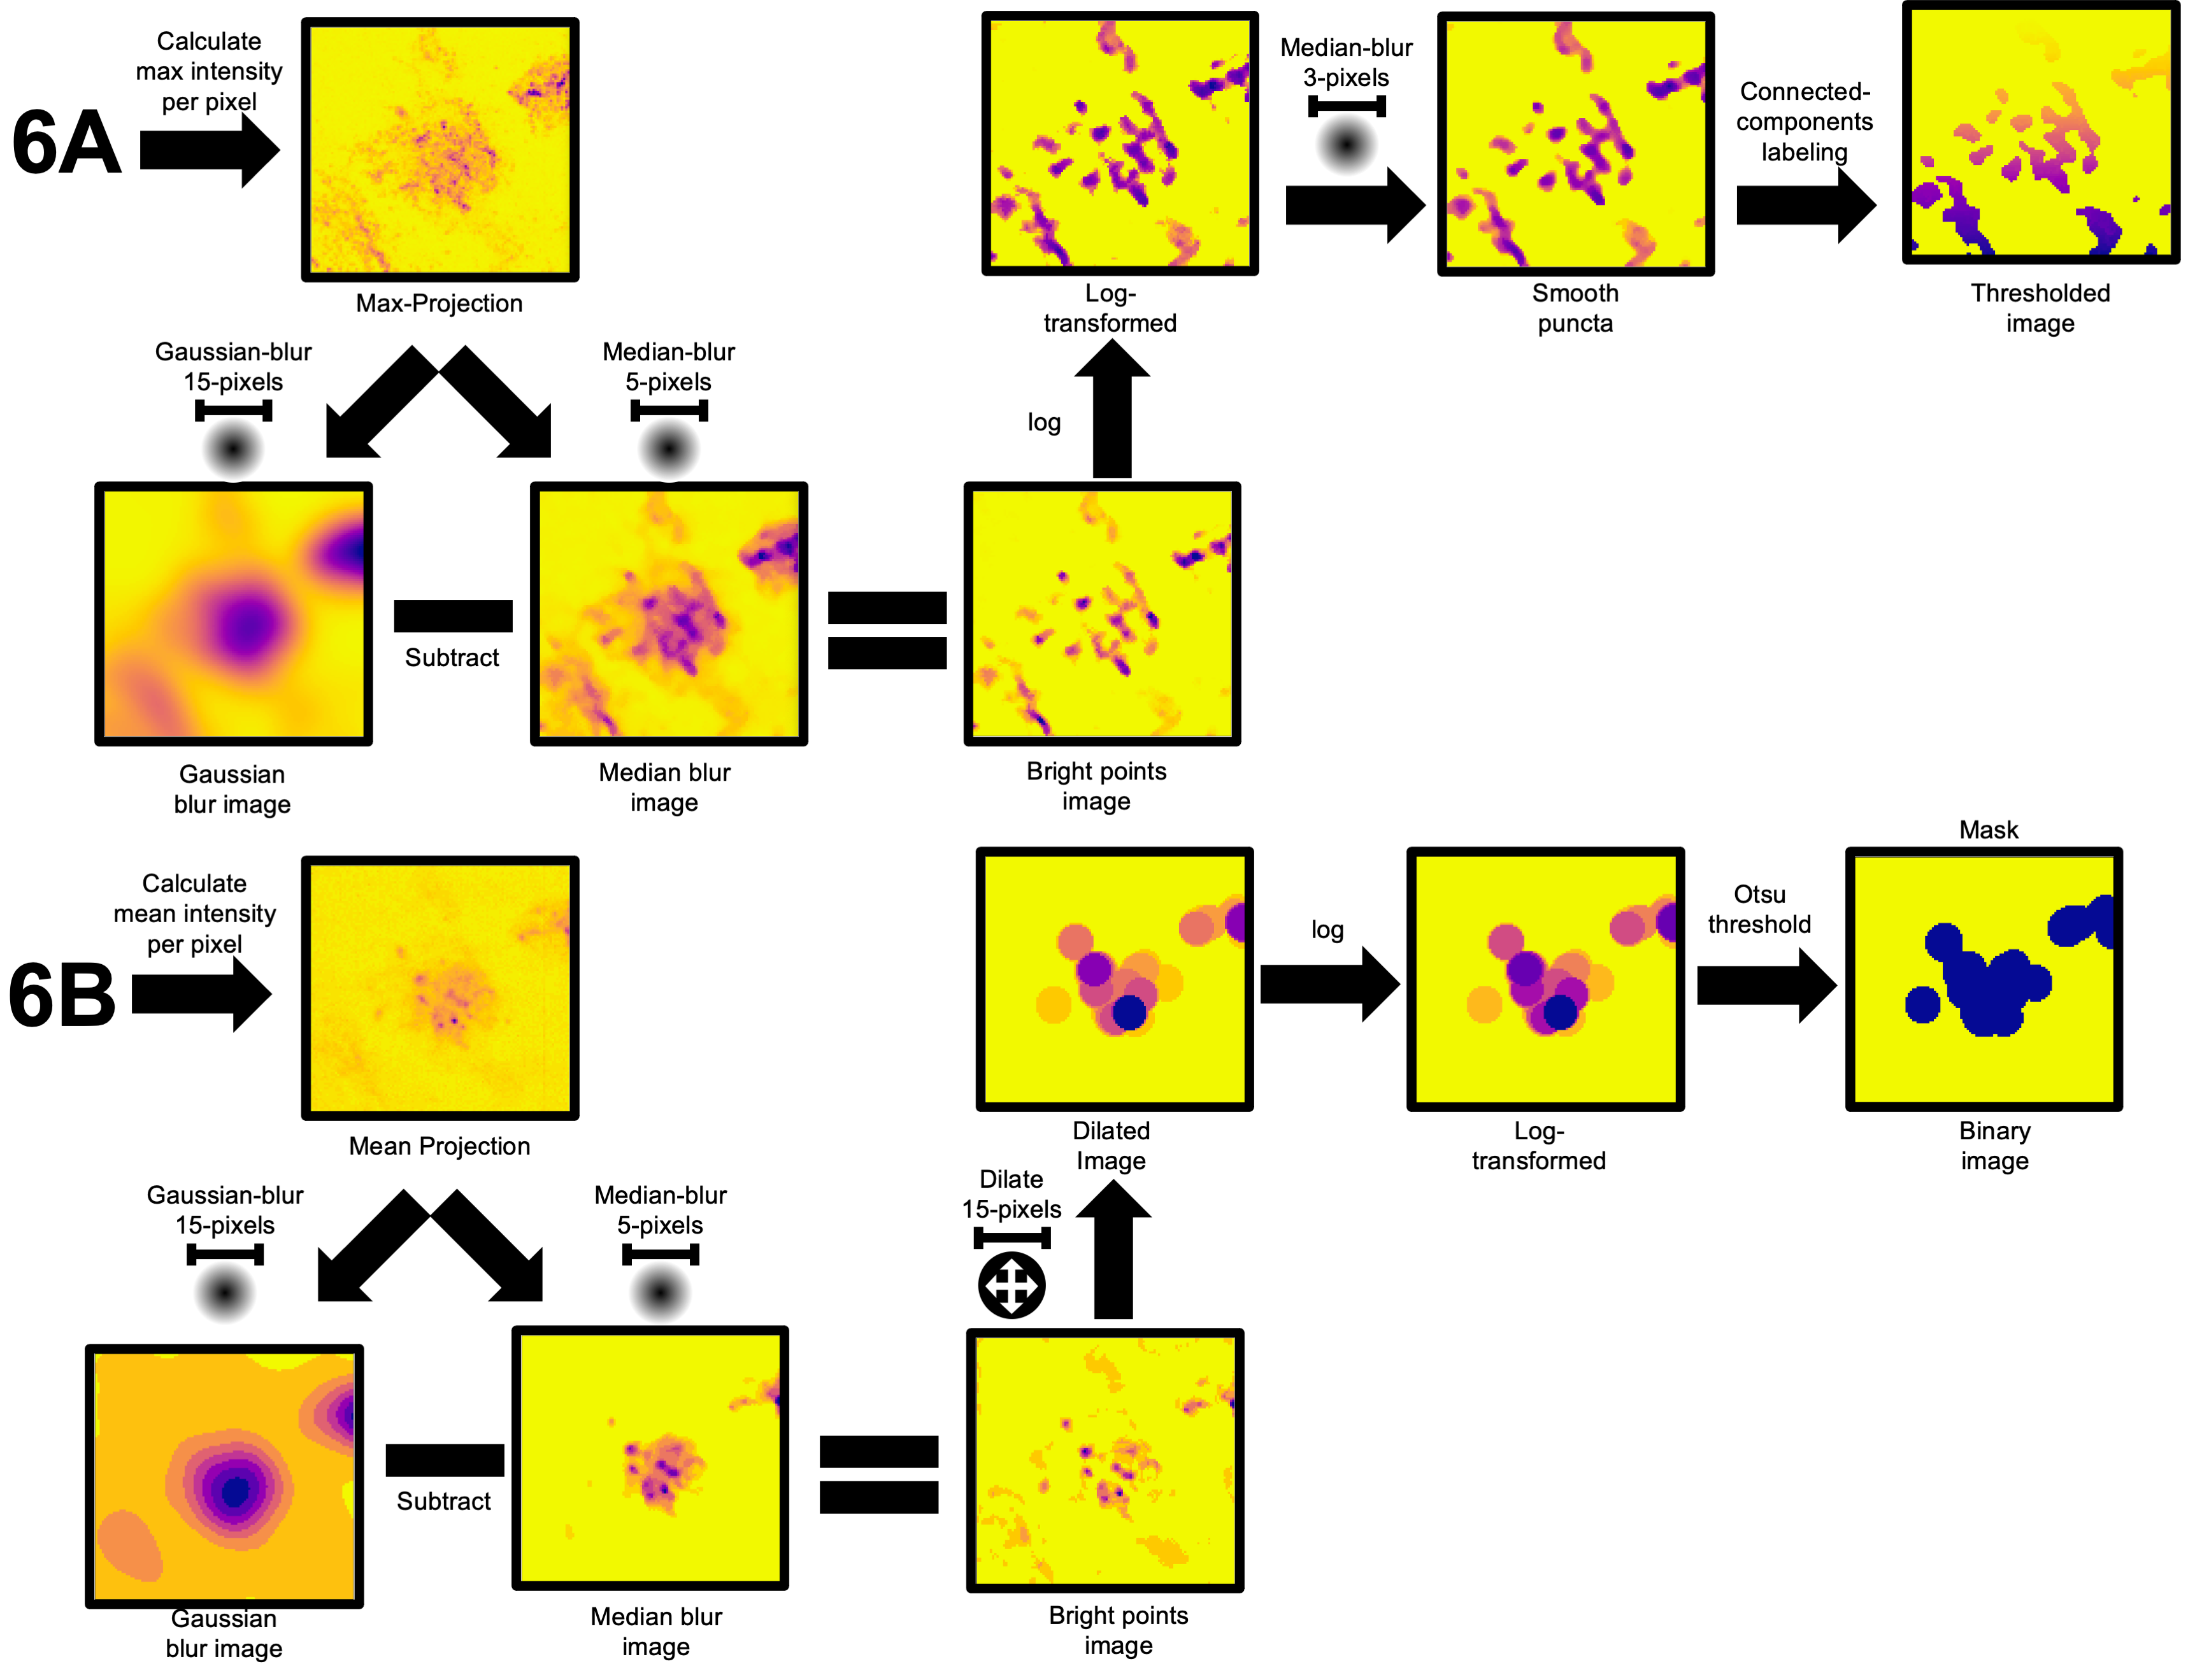
\includegraphics[width=\textwidth, height=\textheight, keepaspectratio]{methods/figS4.png}}
\captionof{figure}[Process for identifying the cell boundary]{\textbf{Process for identifying the cell boundary.} To segment cells present in the image, I used marker-controlled watershed segmentation. One of the requirements of this algorithm is to create a mask that outlines the cell boundary, and a marker that indicates how many cells there are present in the image.
\\
\\
(6A) Starting with the marker, I began by taking the maximum brightness of each pixel. I then duplicated this image, one having a Gaussian blur to estimate a dilated (blow-up) background, and the other had a median blur for estimating the location of puncta. I subtracted the Gaussian from the median image. This resulted in the “bright points image” where puncta are really clear. Because of the wide range in intensities, I log-transformed the image so that the difference between bright and dim points is linear, and not exponential. Then, I smoothed this image using a median blur. This image was thresholded using connected-components labeling. The final image is the marker.
\\
\\
(6B) The mask was estimated using a mean-projection image, that is, the mean intensity of each pixel. Again, I took the Gaussian to estimate the background, and subtracted it from the median blurred image. The resulting image offered sharp puncta. I then dilated these so that all puncta are included within the cell boundary. I log-transformed this image, and thresholded it using Otsu. This is the mask, the cell boundary}
\label{m:S4}
\end{centering}

The next step for segmentation is applying an algorithm called marker-controlled watershed segmentation. To understand how this algorithm works, we need to first examine watershed segmentation

It is called watershed segmentation because it uses the same principle as geographic watershed drainage basins. Therefore, I will first explain geography to better understand image analysis. A watershed is the land that collects water. The drainage basin is where this water flows to, typically rivers though it then makes its way to lakes and ocean. The water is driven to the drainage basin through gravity and elevation. It flows from the highest places (hills) down to the low regions (valleys).

For image analysis, the watershed is calculated using the mask as described above. The distance from the edge (background) needs to be determined. The further away from the background (cell edge), the higher the intensity. This would appear as a hill in an xy-plot (Fig. \ref{m:S5}.Comparison). Between peaks, one can have valleys. In other words, the algorithm calculates the centroid of the binary (thresholded black \& white image) silhouette and treats it as a hill. Then, the further a pixel is from the parent hill, the lower the intensity “elevation.” This distance depression is treated as a valley (Fig. \ref{m:S5}.Comparison). The algorithm then floods the image landscape, which explains why it is called watershed segmentation. The local minima between two centroids (hills) then becomes the boundary (the place where the river flows). However, the output is not perfect at identifying the valleys (Fig. \ref{m:S5}.Comparison).

The marker-controlled watershed is an offshoot of the watershed segmentation. Here, the difference is that the marker (as described above) assists in the identification of hills, that is, the identification of foreground. If there are multiple markers, then more breaks are applied (more regions are identified), and if there is no marker, then there is no boundary. The resulting image is shown in Fig. \ref{m:S5}.6C and how the algorithms compare is shown in Fig. \ref{m:S5}.Comparison.


\begin{centering}
\centering{\includegraphics[width=\textwidth, height=\textheight, keepaspectratio]{methods/figS5.png}}
\captionof{figure}[Identifying individual cells with marker-controlled watershed segmentation for measuring biological replicates]{\textbf{Identifying individual cells with marker-controlled watershed segmentation for measuring biological replicates.}
\\
\\
(Thresholded images) Before segmentation can take place, images need to be in binary format. Two images are required for marker-controlled watershed segmentation: the marker and the mask.
\\
\\
(Thresholded images, marker) The marker identifies where cells are, while the mask indicates the cell outline. Once these two are generated as described before, then watershed segmentation can be used. Watershed segmentation is based on geography. Watersheds are lands where water gets collected. The water then flows up from the hills down into the valleys using gravity. Rivers, lakes and oceans emerge at the drainage basins. This is illustrated on the top right corner.
\\
\\
(Photo) To show how geography informs the watershed segmentation algorithm, I used Lake Lucerne (Switzerland) as an example. For this example, Lake Lucerne is the drainage basin with Bürgenstock (mountain) marked as hills, and the towns of Stansstad and Rotzloch identified as the valley. The black line is to illustrate how watershed segmentation could segment this image.
\\
\\
(Distance maps) With that in mind, the first step for using this algorithm lies in calculating the distances from the cell silhouette (mask) edge. This is termed the distance map and is illustrated above. The most distant places to the cell boundary are treated as hills. Think of them as snow-capped mountains. Then, the depression between two hills (local minima) are treated as valleys. Like glaciers melting, the algorithm then floods the valleys. Wherever rivers emerge is the new cell boundary. For our sample image, classical watershed segmentation is indicated in the middle. However, my script uses marker-controlled watershed segmentation. “Marker-controlled” means that a marker image is used to help find the hills. In my analysis, the marker are the brightest regions (process described above). For the sample image, there are five blobs in the marker image. That means there should be five cells.
\\
\\
(Intensity images) When combined with the distance map, the cell boundaries are more accurately identified, as illustrated on the images.
\\
\\
(Comparison) The rightmost plot is a line profile. The color in the distance maps row of images indicates the distance from the edge. For the line plot, that became the y-axis. The black line in the image is the x-axis, with the origin on the left. The vertical lines in the plot are for indicating where the classical and marker-controlled watershed segmentation algorithms identified cell boundaries. Notice how the marker-controlled watershed segmentation is superior at identifying the hills and the valleys.
\\
\\
The distance maps (bottom row) were drawn for the marker, mask (only for completeness) and with each segmentation algorithm. Then, these were converted into 3D surface plots using the distance from the mask edge. The custom color palette (white-brown-blue) was only to simulate snow-capped mountains and lakes.
\\
\\
(6C) Marker-controlled watershed segmentation of the cells illustrated in figure \ref{m:S4}.}
\label{m:S5}
\end{centering}


\begin{centering}
\centering{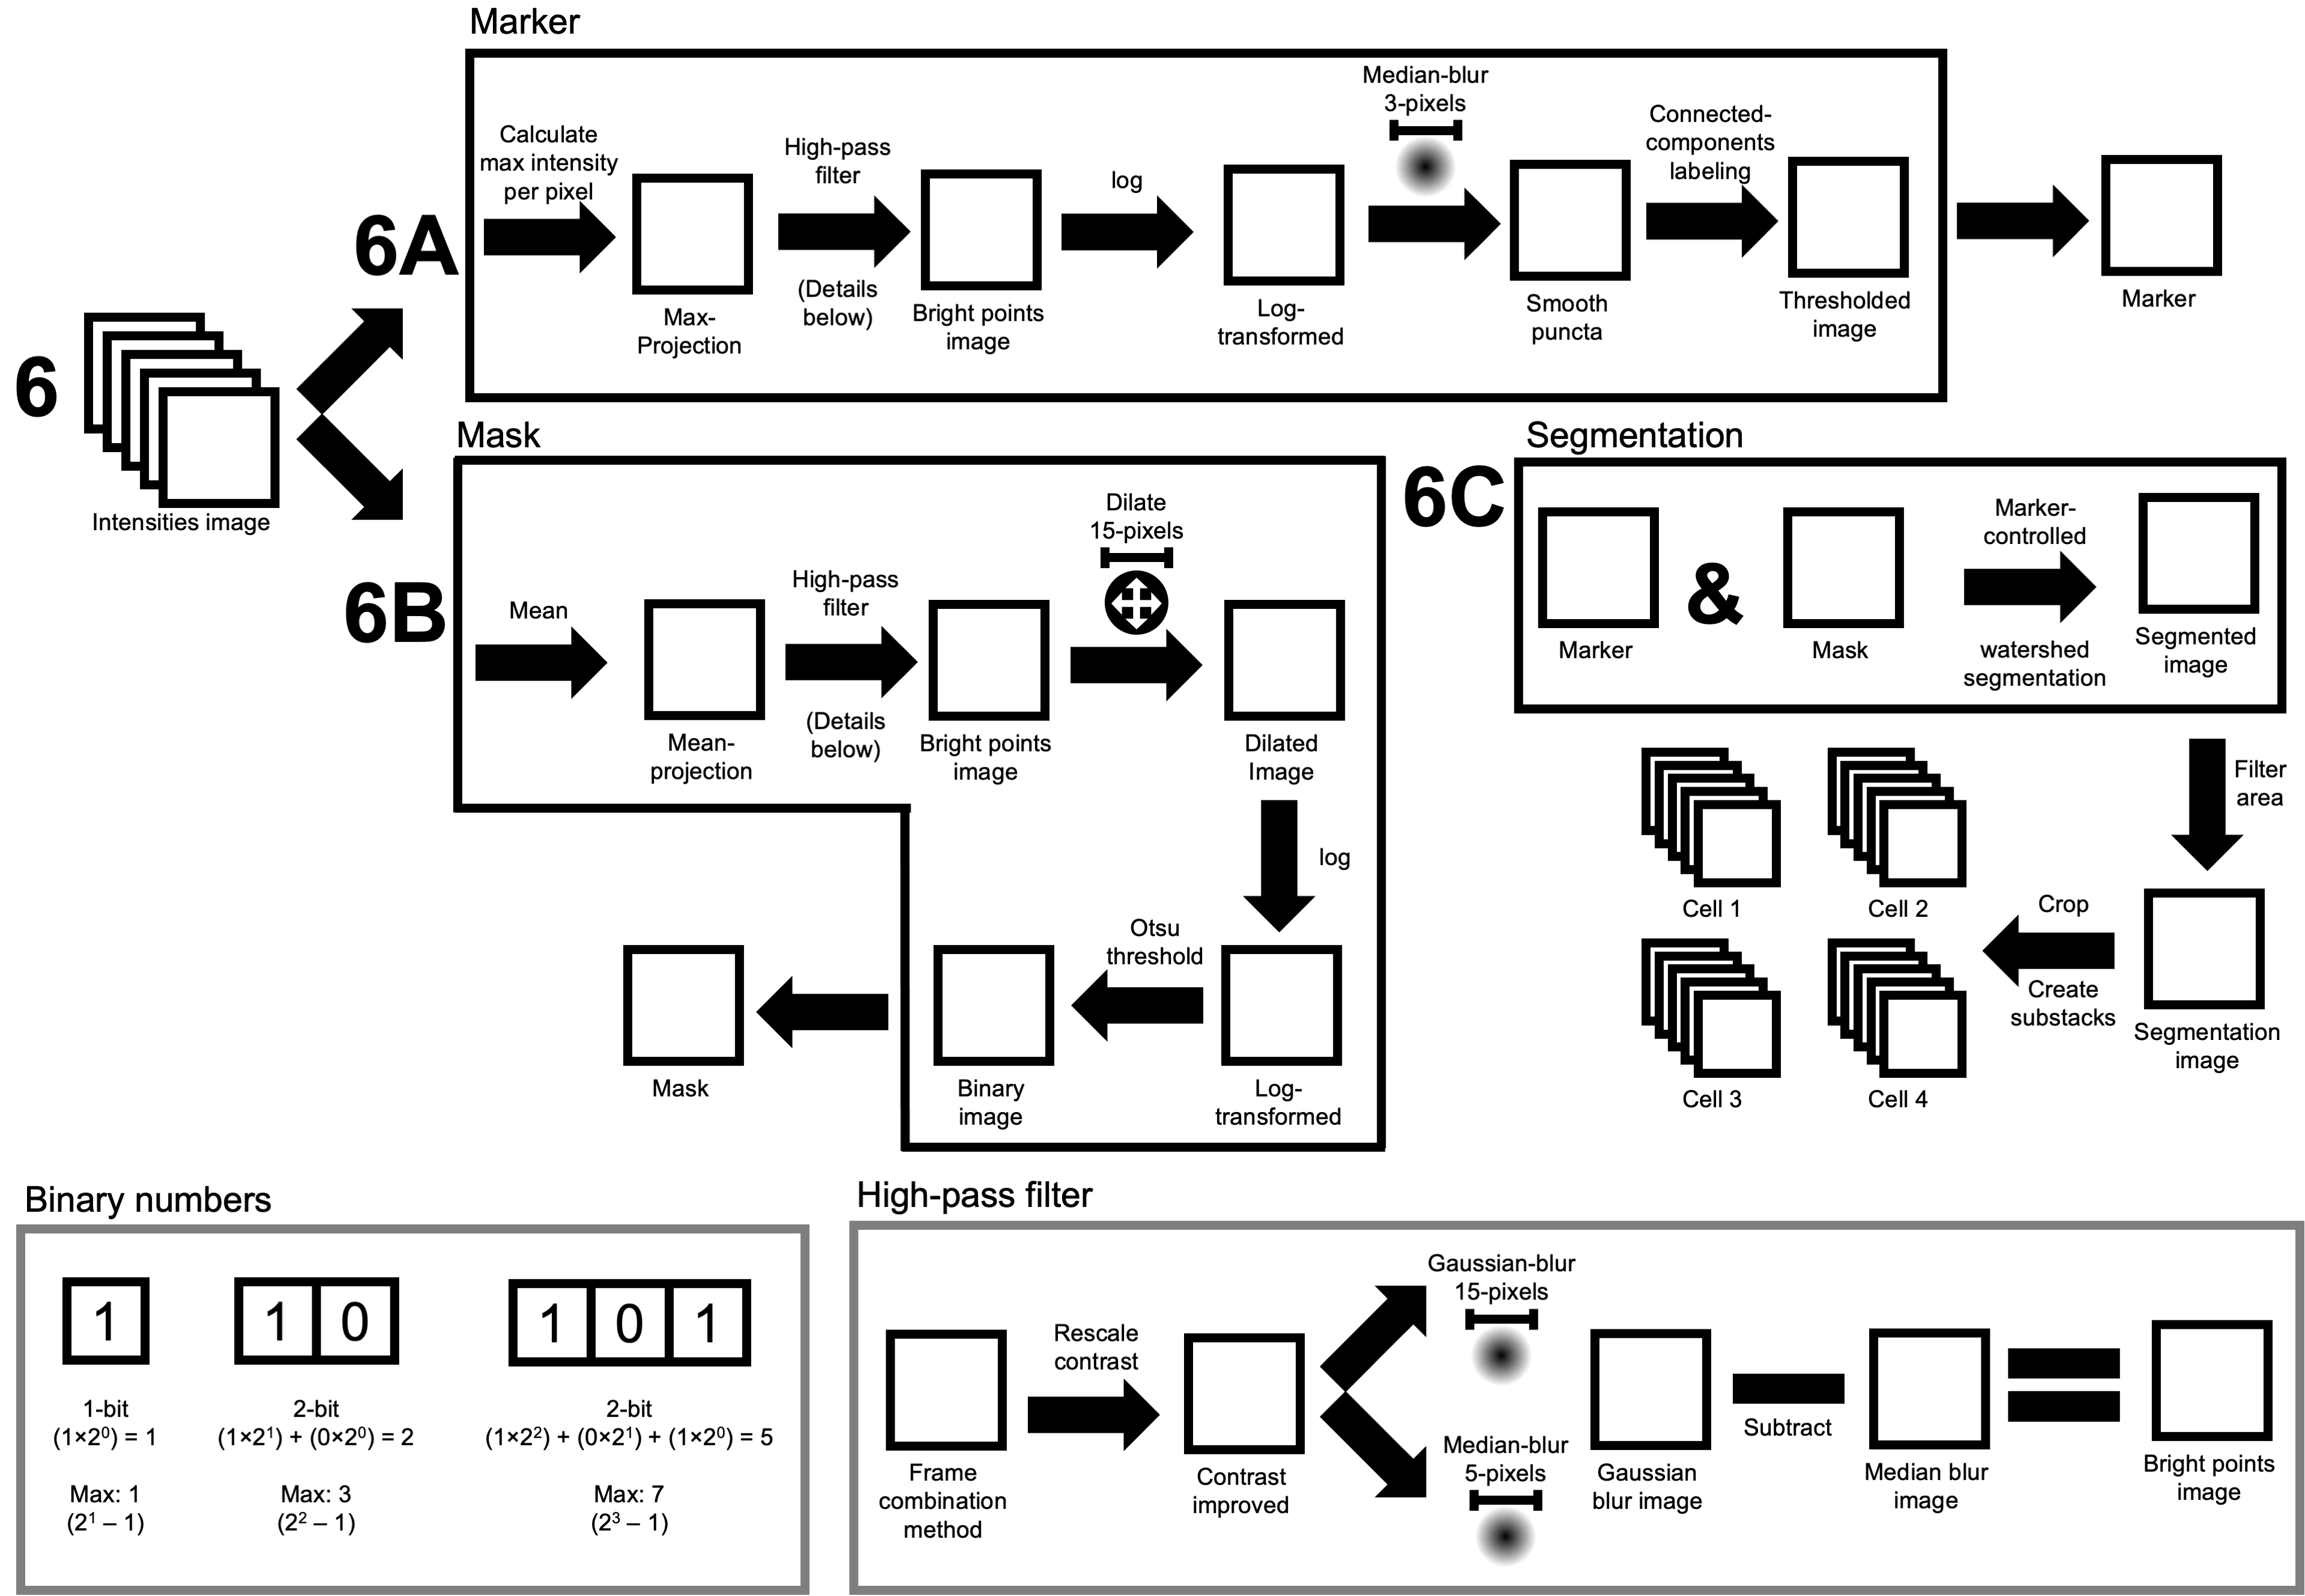
\includegraphics[width=\textwidth, height=\textheight, keepaspectratio]{methods/fig3.png}}
\captionof{figure}[Cell segmentation is performed for calculating biological replicates and speeding-up the pipeline]{\textbf{Cell segmentation is performed for calculating biological replicates and speeding-up the pipeline.} For the segmentation method that we used, we needed to create two images, termed the marker and the mask. The marker indicates where a cell is while the mask indicates the boundary edges.
\\
\\
(6A) The marker is calculated by identifying the brightest regions in the cell. Then, the contrast is improved.
\\
\\
(6) The contrast adjustment rescales the images depending on the TIFF bit depth. This schematic shows how binary numbers (0 or 1) are converted to decimal (1 to 10).
\\
\\
(6B) The mask I used was determined by first averaging all the intensities per pixel. The resulting image, called the mean projection, has its contrast adjusted. The images are split again, one for calculating the Gaussian and another for calculating the median blur. The purpose of this is to calculate the edges. Gaussian blurs blow up images, whereas median blurs keep the structure, that is, they are edge preserving. The Gaussian is subtracted from the median. The resulting image is then log transformed to even out the cell illumination. Lastly, this image is converted into a binary using Otsu thresholding. (6C) For segmentation, I used an algorithm called marker-controlled watershed segmentation. This is a derivation of the watershed segmentation. Watershed segmentation identifies dips in intensities (i.e., local minima, valleys) to identify boundaries/edges. The marker-controlled watershed uses this, but it also uses the bright intensities (i.e., local maxima, hills) to identify how many regions (cells) there are inside the image. The resulting image is the segmentation image. The large original image is then cropped into smaller images using the segmentation image. These smaller images are of individual cells.}
\label{m:3}
\end{centering}

\subsection{TrackMate detects and tracks puncta}
\subsectionmark{TrackMate}
I tracked the puncta with TrackMate (Tinevez et al., 2017), an ImageJ plugin. The first step TrackMate takes is identifying all the puncta in a frame. This is called spot detection. To detect spots, it first fits a 2D Gaussian curve to the entire frame, that is, it applies a Gaussian blur to smooth the image because the next step uses changes (derivatives) in intensity, which are sensitive to noise (Fig. \ref{m:4}.7A).
\begin{equation}
f(x,y) =\text{exp}(-x^2 - y^2)
\end{equation}
The change in intensity is calculated from one pixel to the next. This is known as the derivative (from calculus). \begin{equation}\frac{dx}{dt} = \frac{int - int_0}{t - t_0} = \dot{int}\end{equation} After, it calculates the change of the change, that is, the second derivative using a Laplace operator. \begin{equation}\Delta f = \nabla^2 f = \nabla \cdot \nabla f\end{equation} The Laplace operator is an algorithm for identifying edges (Fig. \ref{m:4}.7A). The result is inverted and the local maxima (brightest pixels in a region) is used to mark the centroid of the puncta and then dilates it to fit a circle of a given pixel size, which for this pipeline is 5-pixels in diameter. This entire method is called Laplacian of Gausian (LoG) filter (Fig. \ref{m:4}.7A). TrackMate then generates a table of puncta (called spots by the software) with xyt (horizontal, vertical, time) coordinates.

To establish which puncta size, there are some important considerations. Merging channels (as shown in the tracking step) introduces a new problem: the channels could potentially be misaligned. Having explained that TrackMate is sensitive to distances, if the spot size parameter is set too tight, part of the puncta would potentially be excluded. For Results~\ref{chapter:p1}, I used 0.44 µm (3-pixel) for the puncta diameter. However, puncta are highly dynamic, exhibiting constant merging and splitting. For this and subsequent chapters, I defined the puncta diameter as 0.73 µm (5-pixels). This allows for more movement flexibility, but a compromise had to be made in that if two puncta are too close, one runs the risk of not being detected.

The next step is to calculate the cost, that is, look at the different frames to identify which puncta are the same. Cost is calculated using the xyt coordinates of each spot to measure the distance to the spots in the next frame (Fig. \ref{m:4}.7B). One distance method used is Euclidean distance. \begin{equation}d(x, y) = \sqrt{(x_{1} + x_{0})^2 + (y_{1} + y_{0})^2}\end{equation} This is done for all puncta, though algorithms take shortcuts to calculate these distances more efficiently, for example, neighbor search. Additionally, criteria are applied, including the intensities.

The closest puncta between frames would be considered to be the same puncta, and the process to identify this is called the linkage. The set of puncta in different frames but considered to be the same are called a track (Fig. \ref{m:4}.7B). The algorithm that I used from TrackMate is called the simple linear assignment problem (LAP) (Fig. \ref{m:4}.7B). An assignment problem is a combination optimization method that finds the best set of puncta that are similar. TrackMate uses additional criteria to find puncta. The first is filtering out spots in different frames that are too far apart. This is called the linking max distance. TrackMate also allows spots to be missing in some frames. This accommodates phenomena like fluorophore blinking. The number of frames that can be skipped is called the gap-closing max frame gap. The maximum linking distance between gaps is called the gap-closing max distance. After running the different algorithms, TrackMate is told to save the files. It uses the extended module (XML) file format (Fig. \ref{m:4}.7C).


\begin{centering}
\centering{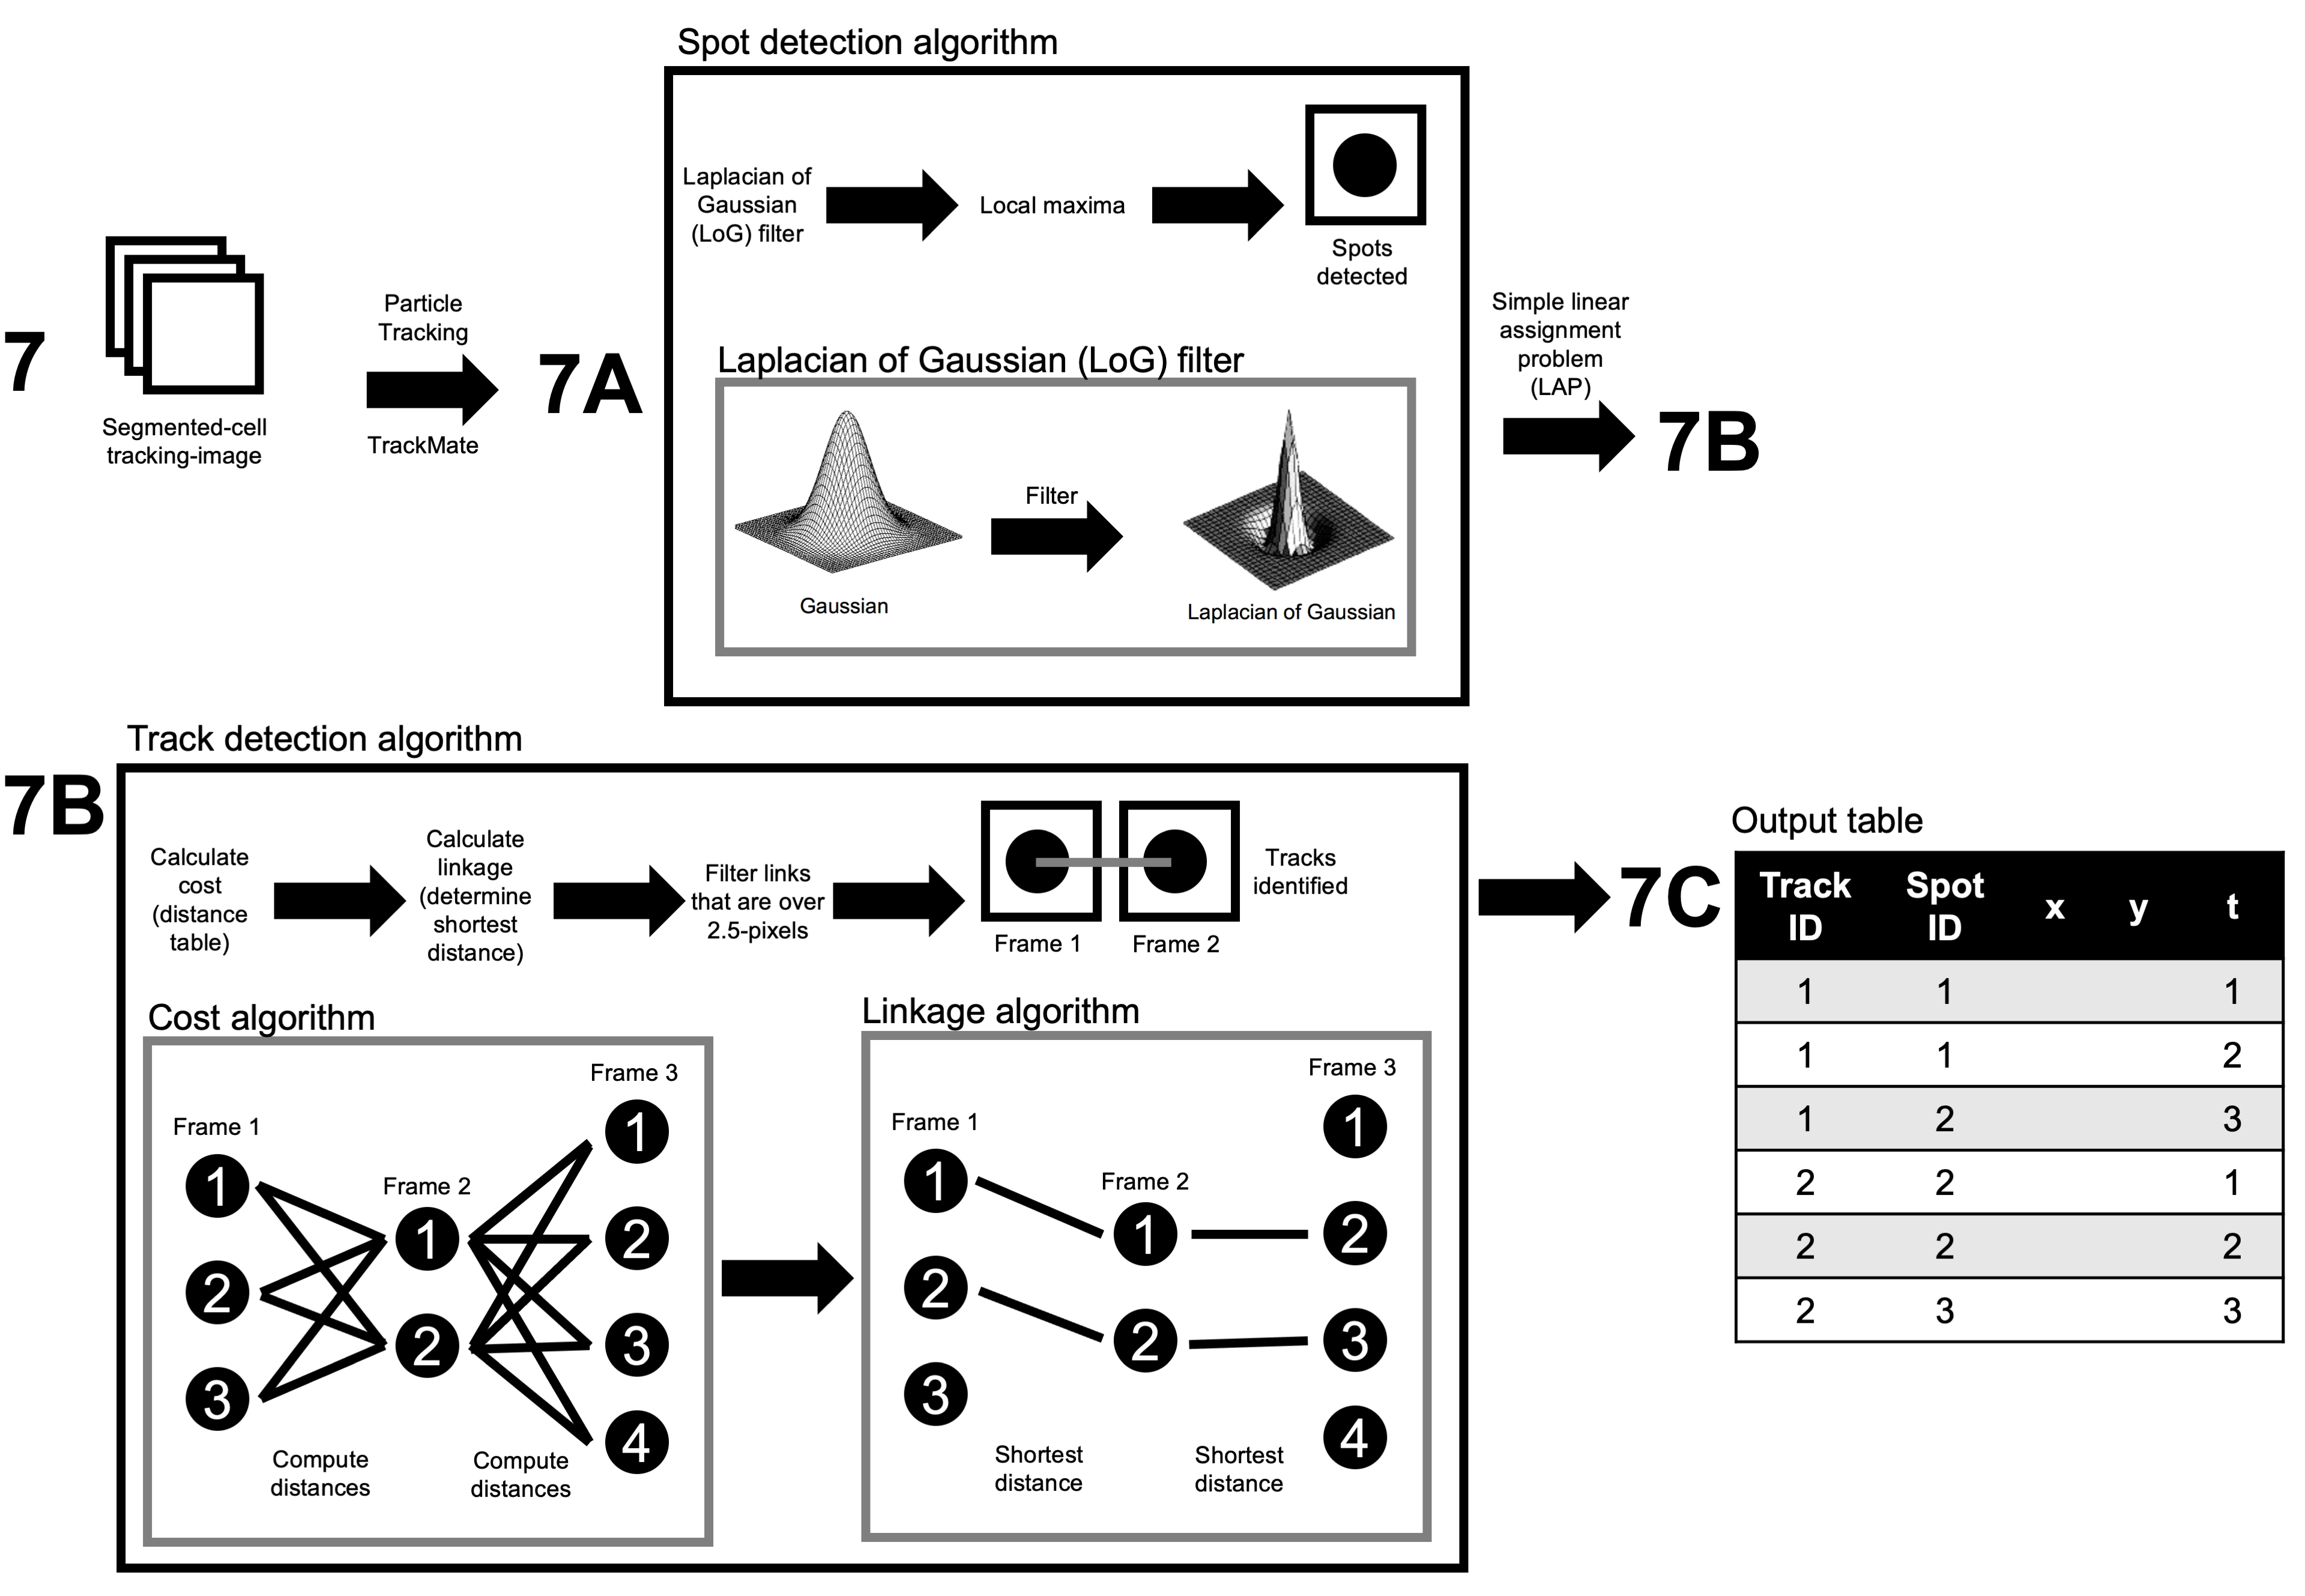
\includegraphics[width=\textwidth, height=\textheight, keepaspectratio]{methods/fig4.png}}
\captionof{figure}[Puncta were identified using TrackMate]{\textbf{Puncta were identified using TrackMate} I used TrackMate to detect puncta and its movements.
\\
\\
(7) The segmented images containing individual cells were fed into the TrackMate plugin of ImageJ.
\\
\\
(7A) The first algorithm TrackMate uses is for detecting puncta. TrackMate calls these spots. It uses a Laplacian of Gaussian filter. This fits a Gaussian (normal) curve and then calculates the edge using a Laplace operator (a differential equation as in Calculus). Lastly, it identifies the local maxima and puts a circle with a defined diameter, 5-pixels in the case of my pipeline. A large table of spots is generated. However, this does not tell us the puncta dynamics, that is, how the puncta grows and shrinks, when it appears and disappears. For this, I need to link puncta in a process TrackMate calls track detection.
\\
\\
(7B) Puncta split and merge, and while there are available TrackMate methods that account for this, this makes the data analysis exponentially more challenging to work around with. It is for simplicity's sake that I used the aptly called simple linear assignment problem (LAP) method for the track detection method. The first step in identifying tracks is to calculate what is called the cost. The cost is the distance between puncta from one frame to the next. For example, in frame 1, I have puncta 1. I calculate its distance to all the puncta in the next frame (Frame 2), that is, puncta 1 and puncta 2 of frame 2. This is done iteratively for all puncta. There are shortcuts algorithms use for calculating cost efficiently. More on this at Tinevez et al., 2017. Using the cost table, the algorithm then calculates the link. That is, it tries to identify the shortest distance. TrackMate allows the user to set a maximum link distance which goes by the same name. Lastly, this is all tabulated and identifies tracks.
\\
\\
(7C) The output information is saved in an XML file which I later extract its data to convert it into a table.}
\label{m:4}
\end{centering}

\subsection{Intensities are measured from the intensity image using TrackMate coordinates}
\subsectionmark{Intensity measured}
Now that the puncta have been tracked in the tracking image, the next step is extracting the fluorescent intensities for the puncta in the different intensity reference images. This is done using R. It is worth mentioning that tracking was done in an image that combines all channels. With this step, channel-specific information is gathered.

The output TrackMate provides is an XML file. I need to convert the XML puncta information into a table, so that it can be easily manipulated in R. TrackMate saves the puncta and track information separately. I extracted the puncta information and paired it with the track information using the puncta (spot) identifiers.

TrackMate allows skipping frames. To fill in the void, I approximated the location of the missing puncta using Euclidean distance. \begin{equation}d(x, y) = \frac{\sqrt{(x_{1} + x_{0})^2 + (y_{1} + y_{0})^2}}{n_\text{gap size}}\end{equation}

With all xyt coordinates available, I extracted the intensities from the intensities reference image. I converted the TIFF image into a matrix. Then, I crop out a square around the puncta (including the puncta). TrackMate used the LoG algorithm to calculate with sub-pixel accuracy the centroid of the puncta. This means I cannot take the centroid of the matrix, draw a circle around it, and sum it. This would offer pixel-level accuracy.

To calculate with sub-pixel accuracy the intensities of the images, I took a different approach. The aforementioned cropped matrix was blown-up, so that I can later use integers to filter-out pixels. I scaled-up (expanded) the image square matrix eleven times ($k = 11 \times$). I chose this factor because this estimation method is 0.387\% similar to a matrix of $k = 51 \times$. I also tried the faster $k = 5 \times$, and it is off by 0.571\% (versus $k = 51 \times$). While it may seem insignificant, error propagates. $k = 11\times$ diminishes the error by 51\%.

Puncta are circular. To segment puncta, I had to generate a circular mask (binary outline, like explained in the segmentation step). I used the equation of a circle \begin{equation}\sqrt{x^2 + y^2} = r\end{equation} and adapted it so that I can make a matrix of pixels with a circle inside a square. \begin{equation}[x - x_0]^2 + [y - y_0]^2 \le r^2\end{equation} This is done because the puncta right now is in a square matrix (generated earlier). However, this equation does not account for the expansion. Therefore, I added a constant $k$ to dilate (blow-up) the circle matrix by a factor of $11\times$ ($k$), so that it has the same dimensions as the blown-up image matrix.

$\begin{aligned}
\relax[x - (r \cdot k)]^2 + [y - (r \cdot k)]^2 &\le (r \cdot k)^2\\
[x - (5\text{ px} \times 11)]^2 + [y - (5\text{ px} \times 11)]^2 &\le (5\text{ px} \times 11)^2 \\
\sqrt{[x - 55\text{ px}]^2 + [y - 55\text{ px}]^2} &\le 55\text{ px}
\end{aligned}$
The resulting matrix was converted into binary:
\begin{equation}
\text{mask}(x,y) =
\left\{\begin{array}{lr}
0, & \text{if }d(x,y)\le (r\cdot k)\\
1, & \text{if }d(x,y) > (r\cdot k)
\end{array}\right.
\end{equation}
where $d(x,y)$ is the pixel in question.

This binary matrix mask is multiplied by the image. The output is a segmented punctum. Multiplying times zero makes the image black and multiplying times one means the input image intensity is kept. This allows me to sum the intensities of the segmented punctum. I then recorded this numerical output as the puncta intensity for a specific channel.

Previously, I had saved the metadata and extracted meaningful information out of it (e.g., TIRF angle, date, proteins in each channel). Now, I combine the metadata, the TrackMate information, and the intensities into a single table. A detailed table content is available in the Methods chapter. I saved this in a comma separated values (csv) table and compressed it using gzip. The intensities of the different channels are added to each spot row using a separate script.

\subsection{The signal is normalized using monomeric fluorophores to estimate puncta stoichiometries}
\subsectionmark{Signal normalization}
The pipeline is now able to self-calibrate (pairing monomeric fluorophore intensities with experimental images obtained in similar conditions) without user input. When the cells are imaged at the microscope (experimental image), we also take images of monomeric fluorophores (calibration image) using the same parameters (angle, direction, laser power, exposure) as the cell imaging. This is done so that I can normalize (calibrate) the experimental images to a reference standard. These calibration images are processed the same way as the experimental images. Then, the pipeline identifies the median brightness of the fluorophore and uses this for normalization by division. The resulting quotient offers an approximation of the stoichiometry (assembly size, oligomer length) in a diffraction-limited puncta which enables us to compare it to other methods (e.g., solved crystal structures).

To automatically determine which calibration image to use, the pipeline uses the metadata of the calibration and experimental images. It pairs the channel name of the calibration and experimental images. For each experimental image, it identifies the best calibration image using the following hierarchy (priority):
\begin{enumerate}
\item Power,
\item Exposure,
\item Angle (in radians),
\item Direction, and
\item Date.
\end{enumerate}
For each step, it calculates the absolute difference between the images metadata, and selects the nearest value before proceeding to the next element in the hierarchy. After it finds the nearest value, it normalizes the intensity. \begin{equation}int_{\text{normalized}} = \frac{int_{\text{punctum}}}{int_{\text{monmeric fluorophore}}}\end{equation}
Where $int$ is intensity.
\subsection{The ligand density is binned so that experimental replicates can be compared}
\subsectionmark{Ligand density}
Protein dynamics are affected by the amount of ligand available in the supported lipid bilayer. Too much ligand, and the assembly process cannot be seen because it happens too fast. This needs to be accounted for when comparing experimental replicates. For each experiment, I estimate the amount of ligand in the supported lipid bilayer. This is done by labeling the ligand with a fluorescent organic dye. Then, I count the number of molecules detected in the field of view and divide it by the area of the image. This is the ligand density. Then, I count the number of puncta seen in the first frames using TrackMate. Because these molecules are freely diffusing, they travel fast. This means motion blur is an issue (motion blur discussed above). The organic dye tolerates photons well. Therefore, I use the lowest exposure possible and the highest laser power that will not burn the camera. For a 16-bit camera, this limit should be be 49,151 a.u. (75\% of the max brightness).
\begin{equation}
\begin{aligned}
\text{max brightness} &= 0.75 \times (2^\text{bit-depth} - 1)\text{ a.u.} \\
& = 0.75 \times(2^{16}-1)\text{ a.u.} \\
& = 0.75 \times (65,535\text{ a.u.}) \\
& = 49,151\text{ a.u.}
\end{aligned}
\end{equation}

Sometimes, the field is dense and individual molecules cannot be counted. To address this issue, we dilute the ratio of labeled to unlabeled protein. Another approach is to capture images continuously to photobleach the molecules. Then, I fit a regression line and use the equation parameters to estimate how many molecules were present at the very beginning. 

From my observations, I have seen that the amount of ligand causes exponential shifts in the protein dynamics. To make this nonlinear system linear, a transformation is in order. Because the data is exponential, a log-transformation will make the ligand density linear. I used $\\log_{\sqrt{10}}(\text{ligand density})$. However, the ligand density must be binned in log-scale.
\begin{equation}
\begin{aligned}
\text{ligand density}_\text{category} &\approx \log_{\sqrt{10}}(\text{ligand density})\\
&\approx \frac{2 \cdot \log(\text{ligand density})}{\log(10)}
\end{aligned}
\end{equation}

\subsection{The data gets tabulated and saved}
\subsectionmark{Saving the data}
Users have expressed interest in filtering puncta that have other puncta nearby to account for splitting and merging. To add this functionality, the pipeline calculates the distance to the nearest spot, and the number of spots within a distance ($d_\text{search}$) using the nearest neighbor search algorithm. The distance threshold ($d_\text{search}$) is calculated using using the equation:
\begin{equation}
d_\text{search} = 6\cdot d_\text{puncta}
\end{equation}

After completing all this, the output is saved in a compressed csv file. CSV files are read row-wise. This means that a lot of unnecessary variables are sometimes read. While I saved different tables with different variables (see Methods), the issue remains. One approach would be to save the table in a format that reads column-wise. One such format is parquet. The installation can be tedious, which is why I did not opt for it (up to this step).

\begin{centering}
\centering{\includegraphics[width=\textwidth, height=\textheight, keepaspectratio]{methods/fig5.png}}
\captionof{figure}[Intensities are extracted from TrackMate coordinates, normalized using the calibration monomeric fluorophores, and saved into a table]{\textbf{Intensities are extracted from TrackMate coordinates, normalized using the calibration monomeric fluorophores, and saved into a table}
\\
\\
(8) TrackMate generated a list of xyt coordinates. To obtain the punctum intensity, I segmented circles out of the different channel images, and used the sum of the pixel intensities per channel as the punctum intensity.
\\
\\
(9) Intensities are in arbitrary units. To be able to compare replicates, as well as the stoichiometry of images against that of solved crystal structures, I normalized the signal to the intensity of monomeric fluorophores. The resulting normalized intensity roughly correlates with the actual stoichiometry of puncta.}
\label{m:5}
\end{centering}

While the scripts compress images, the files can be large. A script is provided to compress everything. This also speeds up the data transfer as too many files slows transfer due to overhead processes.

\subsection{Complex systems can be studied using dimensionality reduction}
\subsectionmark{Complex systems}
\label{section:complex}
Complex systems are intrinsically difficult to understand and model because they can be non-linear, that is, the input-output relationship is not proportional (linear). Instead, it can appear random and unpredictable. Complex systems typically involve multiple components which interact with each other. The protein dynamics I observed can be described as a complex system. In this system, these components are proteins. Complex systems can exhibit feedback, and spontaneous order.

To capture trends, data needs to be summarized while keeping heterogeneity. Two methods through which complex systems can be untangled involve phase portraits and dimensionality reduction.

Dimensionality reduction is the transformation through which high-dimensional space is converted into a low-dimensional space while still retaining the properties of the high-dimensional data. Dimensionality reduction summarizes information by identifying the most important features, and analyzing them. One of the best known dimensionality reduction tools used in biology is principal component analysis (PCA). Dimensionality reduction is particularly useful for complex systems for drawing conclusions when multiple variables influence each other.

Phase portraits are plots of the trajectories of dynamical systems (see Intro~\ref{section:pp}. With the phase portrait, I can identify thresholds, equilibrium points, and regulatory mechanisms.

\subsection{Puncta colocalization can be studied using phase portrait analysis}
\subsectionmark{Phase portrait analysis}
\label{section:pp_method}
The puncta have been measured, but this is only part of the story. To understand how proteins interact with each other within the diffraction-limited puncta, the data needs to be analyzed. I was interested in the dynamics of protein colocalization. Classical protein colocalization microscopy has used correlations between protein intensities per pixel (pixel-matching). The issue here is that dynamics are lost. It is also highly susceptible to noise. Sometimes, a filter is applied so that only the bright pixels of the image are used. Classic colocalization has also used object masking (binary images) to then determine the Manders’ split coefficients. It then calculates the percent overlap from the perspective of each channel. Here, the issue is that the image needs to be thresholded. A decision needs to be made whether it counts or not. Therefore, it has high potential for user bias.

The previous pipeline paired puncta using coordinates, and then looked at their intensities. I made comparisons using the lifetime of the reference protein (MyD88) and the percent colocalization. I also asked how bright the reference protein needs to be to recruit a downstream protein. I calculated the delay between one puncta appearing and the next. However, this approach makes generalizations about the puncta.

I looked at over nine IL-1 pathway proteins. This means my system has nine dimensions. The dynamics are heterogeneous, and not linear, which means the pathway is a complex system. To better understand how individual protein puncta make decisions, I took a soft matter physics approach.

For my phase portraits, I plotted the proteins in phase space, that is, I used the oligomer length of a reference protein (MyD88) and compared it against a query (downstream) protein. I binned the x and y axis using a step size of every 3\times oligomer length. I chose this step size because the trajectories are clear with minimal noise. If there were less than 125 puncta meeting this criteria, then the data was filtered out. This removes noisy data which is not representative of the protein dynamics. The noise can potentially be a random flux which is a type I error (false positive) as a result of poor precision in measurements, and not a true measurement. This filter also focuses the attention of the user into the most frequent events.

Interested in protein assembly, I calculated how each protein grows. The next step involved calculating the change in intensity, that is, the derivative of puncta (Fig. \ref{m:6}). I used a window of $\pm5$ frames, meaning I took a puncta and asked, what was the intensity at five timepoints before and after. I took the difference between these two intensities and the result is the change in intensity (Fig. \ref{m:6}).
\begin{equation}
\Delta int = (\Delta {int}_{t =t_0+t_5}) - ({int}_{t =t_0-t_5})
\end{equation}
To add this to the phase portrait, I looked at all the puncta that met the criteria of a bin, and asked, what is the median intensity change for each protein. The magnitude of growth was indicated using color in the arrows.
\begin{equation}
\text{magnitude} = |\Delta_\text{reference protein}| + |\Delta_\text{query protein}|
\end{equation}
Magnitudes are absolute values. That means it does not differentiate between growth and shrinkage. To account for this, I used the arrow angle to indicate which protein is growing or shrinking. The angle was calculated using the two argument tangent of the change in intensity.
\begin{equation}
\begin{aligned}
\theta &= \text{atan2}(\Delta_\text{query protein}, \Delta_\text{reference protein})\\&=
\left\{\begin{array}{ll}

\text{arctan}(\frac{\Delta_\text{query protein}}{\Delta_\text{reference protein}}), & \text{if }\Delta_\text{reference protein} > 0\\

\text{arctan}(\frac{\Delta_\text{query protein}}{\Delta_\text{reference protein}})+\pi, & \text{if }\Delta_\text{reference protein} < 0 \text{ and }\Delta_\text{query protein} \ge 0\\

\text{arctan}(\frac{\Delta_\text{query protein}}{\Delta_\text{reference protein}})-\pi, & \text{if }\Delta_\text{reference protein} < 0 \text{ and }\Delta_\text{query protein} < 0\\

+\frac{\pi}{2}, & \text{if }\Delta_\text{reference protein} =0 \text{ and }\Delta_\text{query protein}>0\\

-\frac{\pi}{2}, & \text{if }\Delta_\text{reference protein} =0 \text{ and }\Delta_\text{query protein}<0\\

\text{undefined}, & \text{if }\Delta_\text{reference protein} =0 \text{ and }\Delta_\text{query protein}=0

\end{array}\right.
\end{aligned}
\end{equation}


\begin{centering}
\centering{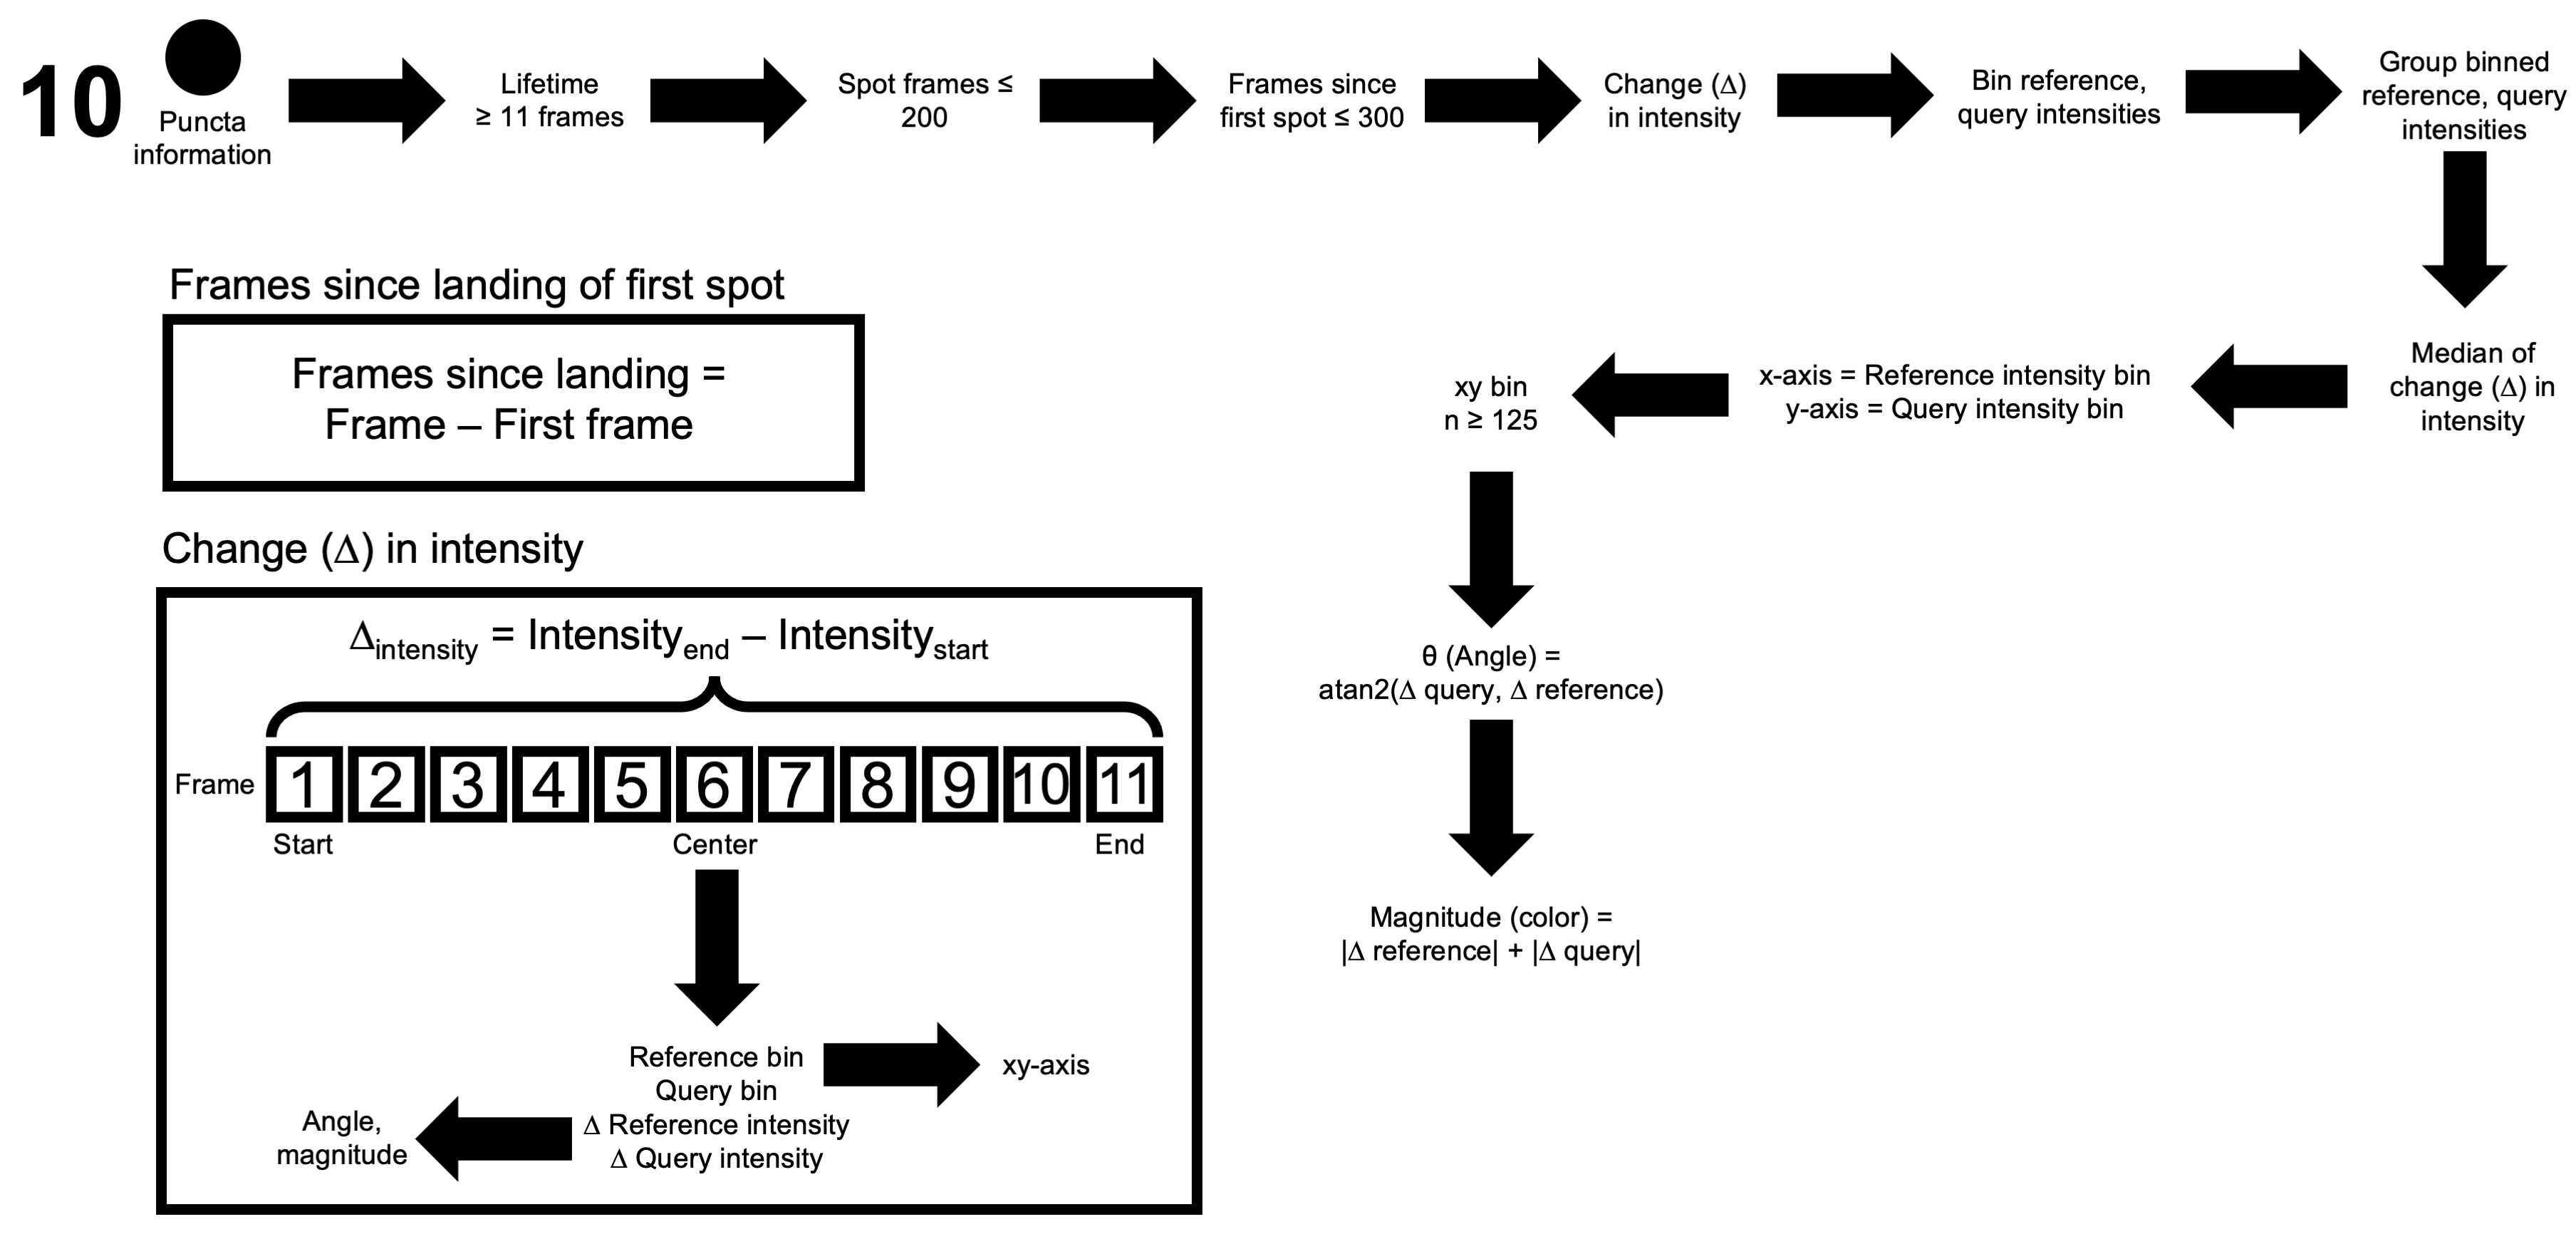
\includegraphics[width=\textwidth, height=\textheight, keepaspectratio]{methods/fig6.png}}
\captionof{figure}[Colocalization using phase portrait analysis can reveal protein dynamics]{\textbf{Colocalization using phase portrait analysis can reveal protein dynamics.} I used phase portrait analysis to analyze the dynamics of protein colocalization. I filtered data so that only puncta with lifetimes over 11 frames (44 s) are included. Then, only the first 200 frames of each puncta were included in the analysis. Another filter limited puncta, so that only those within the first 300 frames since the first spot appeared (frames since landing, see insert) are included. After, I calculated the change in intensity, looking five frames back (lag) and five frames forward (lead) (see insert). The difference in intensities is then recorded per punctum, along with the normalized intensities of the reference and query proteins at the center value. For each binned (every 3\times normalized proteins, per channel) intensity pair (reference, query), I calculated the average (median) change in intensity. Only bins with more than 125 puncta were included. I used the two-argument tangent to calculate the angle of the phase portrait arrow, and the sum of the absolute change in intensities as the arrow magnitude which is indicated in the phase portrait color. The final output is a phase portrait.}
\label{m:6}
\end{centering}

To increase the number of observations, I combined images with similar dynamics. I separated the proteins based on the ligand density (as explained before) because this simple binning method showed similar protein dynamics. To confirm this, I drew the average protein size over time (time traces), color coding the image replicates. After visually confirming that the images show similar dynamics, I rescaled the data using min-max normalization:
\begin{equation}
int_\text{scaled} = \frac{int - int_{1^{st}\,\%}}{int_{99^{th}\,\%} - int_{1^{st}\,\%}}
\end{equation}
and then identified the median min-max values. I used the image whose min-max values were the closest to the median to give normalized values.
\begin{equation}
int_\text{final} = int_\text{scaled} \times int_{99^{th} \%_\text{median}}+int_{1^{st} \%_\text{median}}
\left\{\begin{array}{lr}
0, & \text{if }int_\text{final} < 0\\
int_\text{final}, & \text{if }int_\text{final} \geq 0
\end{array}\right.
\end{equation}
That is, the median calibration values were used to normalize intensities to stoichiometric estimates.

\subsection{The pipeline is cluster-computer compatible with parallelization added to speed up analysis}
\subsectionmark{Parallelization}
The previous pipeline used ImageJ for image processing. One drawback of ImageJ is that few of the processes I used are parallelized, TrackMate being the exception. For this reason, I had to translate the ImageJ functions (for example, file format conversion, median blur) into Python. I used Ray to parallelize my Python scripts, and parallel to parallelize my R scripts. I wrote the scripts so that they can run on Mac, Linux and Windows operating systems (OS). This means the scripts can now run on UNIX-based (OS) high-performance computers (“super-computers”).

I used single nodes from the Raven high-performance computer (HPC) of the Max Planck Computing and Data Facility (MPCDF), Garching, Germany (CPU: 72 cores @ 2.4 GHz, Intel Xeon IceLake Platinum 8360Y; RAM: 256 GB). I also successfully tested it with Cobra of the MPCDF, Garching, Germany (CPU: 40 cores \@ 2.4 GHz, Intel Xeon Gold 6148 Skylake; RAM: 96 GB).

\subsection{Additional improvements to the image analysis pipeline}
\subsectionmark{Additional improvements}
The previous pipeline had over eight scripts that ran independently. It has all been consolidated into one master script that combines Python, ImageJ and R. The image preprocessing (file type conversion, background subtraction) is done in Python using OpenCV, and parallelized with Ray. Puncta are tracked in ImageJ using TrackMate (Tinevez et al., 2017). Lastly, the signal normalization, data consolidation (into one table), and plotting is done in R.

\section{Executing PIRATES: Pipeline for Image analysis with Reference images, Automated Tracking, Extraction of intensities, and Segmentation}
\sectionmark{PIRATES}
\label{section:PIRATES}
We developed a second improved image analysis pipeline for quantifying microscopy images. The second pipeline makes extensive use of parallel processing. It was written in Python 3.8.5, FIJI/ImageJ2 v2 (Schindelin et al., 2012; Rueden et al., 2016) and R 4.0.2 (R Core Team, 2020), and runs on puncta computers.

More details on the pipeline rationale is available in Methods~\ref{chapter:PIRATES_PARLEYS}. Here, I share which scripts are needed and how to enter (input) the parameters into the pipeline.

The pipeline scripts are deposited on GitHub (\url{https://github.com/MJ-Taylor-Lab/DynamicsPipeline}). 

\begin{comment}
Follow this guide, step by step

\subsubsection*{Requirements}
\begin{itemize}
    \item Linux cluster (Raven, Cobra)
    \item R 4.0.2
\end{itemize}

\subsubsection*{Process}

Paste the following in the terminal (**change `username` with your user name**):

Connect to the cluster computer:

\begin{verbatim}
ssh username@raven.mpcdf.mpg.de
\end{verbatim}

\subsubsection*{R packages installation}

Load interpreters

\begin{verbatim}
cd ~
module purge
module load jdk/8.265 gcc/10 impi/2021.2 fftw-mpi R/4.0.2
\end{verbatim}

Install libtiff

\begin{verbatim}
# Install libtiff
mkdir libtiff
cd libtiff
wget https://download.osgeo.org/libtiff/tiff-4.3.0.tar.gz
tar -xvf tiff-4.3.0.tar.gz
mkdir install
cd tiff-4.3.0
mkdir compile
cd compile
# Change username here
../configure --prefix=/u/username/libtiff/install
make
make install
# Change username here
export PKG\_CONFIG\_PATH=/u/username/libtiff/install/lib/pkgconfig/
\end{verbatim}

Change directory to home. Type `~` and press [Enter]

Load R. Enter `R` on the terminal and press [Enter]

Paste the following in the R console inside the terminal:

\begin{verbatim}
if("pacman" %in% rownames(installed.packages()) == FALSE)
{install.packages("pacman")}
\end{verbatim}

When prompted, type `yes` to install and `yes` to create a personal library. After, another prompt will appear. Select which repository you would like to use. Enter `1` (cloud) and then press [Enter]

Then, paste the following:

\begin{verbatim}
pacman::p\_load(ijtiff)
\end{verbatim}


After, paste the following:

\begin{verbatim}
pacman::p\_load(XML)
\end{verbatim}

Lastly, paste the following:

\begin{verbatim}
pacman::p\_load(dplyr, stringr, parallel, tidyr, data.table, ff, dtplyr, compiler, changepoint, R.utils, lemon, ggquiver, ggplot2, ggdark, scales, ggforce, viridis, RcppRoll, metR)
\end{verbatim}

Exit R by typing `q()` and then `N` to not save

\subsubsection*{Python packages installation}

Create Python Packages list. Open the terminal text editor, then type `nano` and paste:

\begin{verbatim}
aiohttp
aiohttp-cors
aioredis
appdirs
async-timeout
attrs
blessings
boto3
botocore
cachetools
certifi
chardet
click
colorama
colorful
cycler
decorator
distlib
et-xmlfile
filelock
future
google-api-core
google-auth
googleapis-common-protos
gpustat
grpcio
hiredis
idna
imageio
imglyb
jgo
jmespath
JPype1
jsonschema
kiwisolver
matplotlib
msgpack
multidict
nd2reader
networkx
numpy
nvidia-ml-py3
opencensus
opencensus-context
opencv-python
openpyxl
packaging
pandas
Pillow
PIMS
pims-nd2
pipenv
prometheus-client
protobuf
psutil
py-spy
pyasn1
pyasn1-modules
pyparsing
pyrsistent
python-dateutil
pytz
PyWavelets
PyYAML
ray
requests
rsa
s3transfer
scikit-image
scipy
scyjava
six
slicerator
tifffile
typing-extensions
urllib3
virtualenv
virtualenv-clone
xarray
xlrd
xmltodict
yarl
\end{verbatim}

Close nano:
\begin{itemize}
    \item Press [CTRL] + [X] to close
    \item Press [Y] to save
    \item Save as `python\_requirements.txt`
\end{itemize}

> **Optional**: You may use screen to let process run on the background
>    * Type `screen`
>    * Wait 5s to load
>    * Press [CTRL] + [A] and let go
>    * Press [D]
>    * To resume, type `screen -r`
>> \_If there's more than one screen, type `screen -r` . to get the index of screens and then replace 00000 with the index (`screen -r 00000`)\_

\begin{verbatim}
# Install ImageJ
wget https://downloads.imagej.net/fiji/latest/fiji-linux64.zip
unzip fiji-linux64.zip

# Install conda
wget https://repo.anaconda.com/miniconda/Miniconda3-latest-Linux-x86\_64.sh
chmod +x Miniconda3-latest-Linux-x86\_64.sh
./Miniconda3-latest-Linux-x86\_64.sh
export PATH=~/miniconda/bin:$PATH
source ~/miniconda3/bin/activate
export PATH="/miniconda3/bin":$PATH

# Follow Terminal instructions to install conda

# Create conda environment
conda create -n dynamics\_pipeline python=3.8 anaconda
\end{verbatim}

Then paste,

\begin{verbatim}
# Create conda environment
conda activate dynamics\_pipeline

# Install conda packages
conda install -c conda-forge setuptools
conda install -c conda-forge javabridge
conda install -c conda-forge libxml2
pip install glib

# Install Python packages
python -m pip install --user -r python\_requirements.txt
\end{verbatim}

\subsubsection*{Git installation}

Paste the following and rename the last element to yours:

\begin{verbatim}
git config --global user.name "username"
git config --global user.email email@mpcdf.mpg.de
ssh-keygen -t rsa -b 4096 -C "name@raven.mpcdf.mpg.de"
\end{verbatim}

Press [Enter] to skip some steps and get the ssh key. Then, copy the entire block of string from start to finish, including the \_ssh-rsa\_ and the ending name . Use `cat /u/username/.ssh/id\_rsa.pub` and change **user\_path** accordingly

Sign-in to GitHub, https://github.com/login

Paste the key into GitHub, https://github.com/settings/keys

\begin{itemize}
    \item New SSH key
    \item Type in the cluster name as **Title** and paste the key under **Key**
\end{itemize}

Create a directory to save the pipeline scripts

\begin{verbatim}
mkdir dynamics\_pipeline
cd dynamics\_pipeline
\end{verbatim}

Paste the following in the terminal to clone the pipeline:

\begin{verbatim}
git init
git remote add origin git@github.com:MJ-Taylor-Lab/DynamicsPipeline.git
git remote set-url origin git@github.com:MJ-Taylor-Lab/DynamicsPipeline.git
git fetch --all
git pull origin master
\end{verbatim}

---
\subsection*{Image Analysis Pipeline}
\end{comment}

\subsubsection*{Input}
The input data goes into ~/new\_pipeline/pending\_processing/batch\_date/Input/

\begin{table}[htb]
  \centering
  \caption{Numbers which will be constant throughout the analysis}
  \label{tab:constants}
  \begin{tabular}{ | l | c | p{5cm} | }
    \hline
    \textbf{Parameter} & \textbf{Value} & \textbf{Comments} \\ \hline
    \texttt{tiff\_compression\_level} & 5 & out of 10 \\ \hline
    \texttt{cell\_diameter} & 25 & px, odd number \\ \hline
    \texttt{puncta\_diameter} & 5 & px, odd number \\ \hline
  \end{tabular}
\end{table}

\begin{table}[htb]
  \centering
  \caption{The dark frame is the camera noise. This typically is 1000 frames averaged, though 50 frames could do, so long as the standard deviation does not change with more images added. It should be at the same exposure as the images using the same camera as the microscopy images. Thus, one image could be used for multiple channels.}
  \label{tab:dark\_frames}
  \begin{tabular}{ | l | c | }
    \hline
    \textbf{Image} & \textbf{Exposure} \\ \hline
    \texttt{20201026 Darkfield 200ms binned.tif} & 200 ms \\ \hline
    \texttt{20201026 Darkfield 50ms binned.tif} & 50 ms \\ \hline
    \texttt{20201026 Darkfield 100ms binned.tif} & 100 ms \\ \hline
  \end{tabular}
\end{table}

\begin{table}[htb]
  \centering
  \caption{Directory paths}
  \label{tab:directories}
  \begin{tabular}{ | l | p{10cm} | }
    \hline
    \textbf{Contains} & \textbf{Path} \\ \hline
    \texttt{input} & \texttt{\textasciitilde/Input} \\ \hline
    \texttt{processing} & \texttt{\textasciitilde/Processing} \\ \hline
    \texttt{output} & \texttt{\textasciitilde/Output} \\ \hline
    \texttt{dark\_frames} & \texttt{\textasciitilde/dark\_frames} \\ \hline
    \texttt{flat\_fields} & \texttt{\textasciitilde/flat\_fields} \\ \hline
    \texttt{ImageJ} & \texttt{\textasciitilde/Fiji.app/ImageJ-linux64} \\ \hline
  \end{tabular}
\end{table}


\subsubsection*{exclusion\_channels.csv}
\begin{tabular}{|c|}
    \hline
    value \\
    \hline
    IL-1 \\
    Brightfield \\
    WideField \\
    \hline
\end{tabular}

\subsubsection*{images.csv}
\begin{tabular}{|l|l|l|l|l|l|l|l|l|l|l|l|}
    \hline
    image & cohort & segment\_with & ligand & ligand\_density & trackmate\_max\_link\_distance & trackmate\_threshold & trackmate\_frame\_gap & T Cy5 protein\_name & T GFP protein\_name & T RFP protein\_name & WideField protein\_name \\
    \hline
    20211218 0p8nM 069-1R\_TRAF6\_MyD88 Grid\_1um\_11mol 001.nd2 & MyD88 TRAF6 1um\_grid & MyD88 & 0.8 nM IL-1 & 11 & 5 & 1.5 & 5 & IL-1 & MyD88 & TRAF6 & Brightfield \\
    20211218 GFP calibration\_10pct\_60ms 005.nd2 & Calibrations & GFP &  &  & 2.5 & 1.5 & 5 & IL-1 & GFP & mScarlet & Brightfield \\
    20211218 mScarlet calibration\_10pct\_60ms 001.nd2 & Calibrations & mScarlet &  &  & 2.5 & 1.5 & 5 & IL-1 & GFP & mScarlet & Brightfield \\
    \hline
\end{tabular}

\begin{comment}
\subsection*{Run}

Connect to the cluster computer:

\begin{verbatim}[language=bash]
ssh username@raven.mpcdf.mpg.de
\end{verbatim}

If you need the latest scripts, paste in the Terminal:

\begin{verbatim}[language=bash]
cd dynamics\_pipeline
git pull origin master
\end{verbatim}

\subsubsection*{SLURM Instructions}

Pull the scripts before using \lstinline{git pull origin master} and modify the parameters of \lstinline{submit\_node.sh} accordingly.

\begin{verbatim}
#!/bin/bash -l
    
#SBATCH -o ./job.out.%j
#SBATCH -e ./job.err.%j
#SBATCH -D ./
#SBATCH -J 20211218
#SBATCH --mail-type=ALL
#SBATCH --mail-user=email@mpcdf.mpg.de
#SBATCH --nodes=1
#SBATCH --ntasks-per-node=1
#SBATCH --cpus-per-task=72
#SBATCH --time=24:00:00
    
# Load all needed packages
module purge
module load jdk/8.265 gcc/10 impi/2021.2 fftw-mpi R/4.0.2
echo 'modules loaded'
conda activate dynamics\_pipeline
echo 'conda activated'
    
# Specify parameters
## Path of parameters table
## Change username to your cluster user name
path=$'/raven/u/username/new\_pipeline/pending\_processing/batch\_date/Input/parameter\_tables'
    
## Scripts folder
## Change username to your cluster user name
cd /raven/u/username/dynamics\_pipeline
    
## Cores for parallel processing in R
export OMP\_NUM\_THREDS=144
    
# Run scripts
## Python scripts
python mission\_control.py $path 12
    
## Run R Scripts
Rscript --vanilla --verbose r\_scripts/extract\_intensity.R $path
Rscript --vanilla --verbose r\_scripts/colocalization.R $path
Rscript --vanilla --verbose r\_scripts/compile\_tables.R $path
#Rscript --vanilla --verbose r\_scripts/compress\_everything.R $path
    
sleep 10
\end{verbatim}

Paste `sbatch submit\_node.sh` to submit to SLURM.

\subsection*{Output}

\end{comment}
\subsubsection*{Essentials.csv.gz}

\textbf{Identification}

\begin{itemize}
    \item RELATIVE\_PATH: Relative path to cell folder. Simplifies address to source images and parameters
    \item COHORT: Cell line name (proteins tagged) plus any perturbations (for example, grids, inhibitors)
    \item IMAGE: Name of image. Our format is:
    \begin{itemize}
        \item Date (YYYYMMDD)
        \item Ligand concentration + density
        \item Cell line name
        \item Plate + well number
    \end{itemize}
    \item PROTEIN: Protein name
    \item UNIVERSAL\_TRACK\_ID: Unique cluster identifier, computed as:
    \begin{itemize}
        \item IMAGE + '...'
        \item CELL + '...'
        \item PROTEIN + '...'
        \item TRACK\_ID
    \end{itemize}
    \item UNIVERSAL\_SPOT\_ID: Unique spot identifier, computed as:
    \begin{itemize}
        \item UNIVERSAL\_TRACK\_ID + '...'
        \item FRAME
    \end{itemize}
    \item ANALYSIS\_TIME\_STAMP: Date and time of analysis completion
\end{itemize}

\subsubsection*{Temporal measurements}

\begin{itemize}
    \item TIME: Time in seconds from when image acquisition started
    \item FRAME: Image frame number
    \item TIME\_SINCE\_LANDING: Time in seconds since the first spot in the cell appeared
    \item FRAMES\_SINCE\_LANDING: Frames since the first spot in the cell appeared
    \item TIME\_ADJUSTED: Cluster time in seconds
    \item FRAMES\_ADJUSTED: Cluster time in frames
    \item LIFETIME: Cluster time in seconds. May need to be recalculated after passing fi
\end{itemize}

I recommend calculating the fluorophore bleaching rate. Filter data (FRAMES\_SINCE\_LANDING, FRAMES\_ADJUSTED) based on the results of this parameter.

\subsubsection*{Spatial measurements}

\begin{itemize}
    \item ABSOLUTE\_POSITION\_X: X-coordinate of cluster centroid in microns
    \item ABSOLUTE\_POSITION\_Y: Y-coordinate of cluster centroid in microns
    \item CELL\_AREA: Area of the cell in microns
    \item NEAREST\_SPOT: Distance to nearest cluster in pixels
    \item SPOTS\_WITHIN\_RADIUS: Number of spots within puncta radius
\end{itemize}

\subsubsection*{Amount of substance data}

\begin{itemize}
    \item NORMALIZED\_INTENSITY: Estimate number of molecules of the reference protein
    \item STARTING\_NORMALIZED\_INTENSITY: Starting amount of the reference protein
    \item MAX\_NORMALIZED\_INTENSITY: Max amount (brightness) of the relative protein
    \item START\_TO\_MAX\_INTENSITY: Growth, measured as max – start amount
    \item COMPLEMENTARY\_PROTEIN\_\#: Protein in other channel(s)
    \item COMPLEMENTARY\_TOTAL\_INTENSITY\_\#: Brigness of other channel in arbitrary units
    \item COMPLEMENTARY\_NORMALIZED\_INTENSITY\_\#: Estimate number of molecules of the query protein
    \item COMPLEMENTARY\_UNIVERSAL\_SPOT\_ID\_\#: UNIVERSAL\_TRACK\_ID of the query protein spot
\end{itemize}


\subsubsection*{Parameters.csv.gz}

\subsubsection*{Other information}
\begin{itemize}
    \item \texttt{RELATIVE\_PATH}: Identifies cell + protein in question
    \item \texttt{LIGAND}: Ligand that stimulates 
    \item \texttt{SEGMENT\_WITH}: Protein name of the channel that was used for segmenting the cells from the image
\end{itemize}

\subsubsection*{Fluorophore data}
\begin{itemize}
    \item \texttt{CALIBRATION\_IMAGE}: Image used for fluorophore normalization
    \item \texttt{CALIBRATION\_TOTAL\_INTENSITY}: Median brightness of the fluorophore in arbitrary units
    \item \texttt{CALIBRATION\_STANDARD\_DEVIATION}: Variance of the brightness of the fluorophore in arbitrary units
\end{itemize}

\subsubsection*{Microscope information}
\begin{itemize}
    \item \texttt{CHANNEL}: Microscope channel
    \item \texttt{POWER}: Laser power
    \item \texttt{EXCITATION}: Peak wavelength of laser excitation
    \item \texttt{EMMISION}: Peak wavelength of emmision filter
    \item \texttt{ANGLE}: TIRF critical angle in degrees
    \item \texttt{DIRECTION}: Refraction direction in degrees (angle)
    \item \texttt{FOCUS}: Objective z-axis distance (not the stage z-axis)
    \item \texttt{OBJECTIVE}: Objective magnifying power
    \item \texttt{TIME\_START}: Timestamp of when imaging acquisition started
    \item \texttt{FRAME\_RATE}: Number of frames per second (Hz)
\end{itemize}

\subsubsection*{Spatial information}
\begin{itemize}
    \item \texttt{WIDTH}: Image width in microns
    \item \texttt{HEIGHT}: Image height in microns
    \item \texttt{CALIBRATION\_UM}: Pixel size in microns
    \item \texttt{CELL\_DIAMETER}: Estimate cell diameter, as entered in pipeline. Used in the cell median-filter step, whose resulting image is \texttt{PROTEIN + '\_intensity\_ref.tif'}
    \item \texttt{PUNCTA\_DIAMETER}: Estimate puncta diameter, as entered in pipeline. Used in the puncta median-filter step, whose resulting image is \texttt{PROTEIN + '\_tracking\_ref.tif'}
    \item \texttt{SPOT\_RADIUS\_LIMIT}: Radius of spot
    \item \texttt{CELL\_POSITION\_X}: X-coordinate of the cell in the image
    \item \texttt{CELL\_POSITION\_Y}: Y-coordinate of the cell in the image
\end{itemize}

\subsubsection*{TrackMate information}
\begin{itemize}
  \item \verb|TRACKMATE_THRESHOLD|: TrackMate's threshold
  \item \verb|TRACKMATE_FRAME_GAP|: TrackMate's maximum frame gap between spots appearing at a location (missed detection)
  \item \verb|TRACKMATE_GAP_LINK_DISTANCE|: TrackMate's maximum frame gap distance in pixels between spots appearing at a location (missed detection)
  \item \verb|TRACKMATE_MAX_LINK_DISTANCE|: Maximum distance in pixels before the spot gets classified as a new distinct track (cluster)
\end{itemize}


\subsection{Image preprocessing}
To quantify the microscope images, we ran our pipeline on the Raven supercomputer of the Max Planck Society (\url{https://www.mpcdf.mpg.de/services/supercomputing/raven}). The entire pipeline is executed from the mission\_control.py script. Input parameters need to be saved as csv documents (\url{https://github.com/MJ-Taylor-Lab/DynamicsPipeline\#input}). Each subfolder on the pipeline is named after the purpose. Within them, there are two files: parameters.py (for input) and operations.py (functions).

The first step is the ‘conversion’ from Nikon's proprietary ND2 to the universal TIFF. We also saved the metadata as csv and txt.

The second set of scripts is the ‘background’ removal. We removed the average dark-frame (camera noise) image using the same or closest exposure to our experimental images. The dark-frame must be the first background removed because the source of the dark-frame image is the camera noise. For obtaining the dark frame image, a thousand frames were captured with the shutter closed and then averaged. The number of frames depends on when the standard deviation remains unchanged (the same) even with a larger N (more images). The dark frame image was subtracted. Then, two image stacks were generated, one for obtaining fluorescent intensities and another for particle tracking.

Starting with the intensities image stack (cytosolic background eliminated), we blur the image stack using a median filter (blur). We use a median filter because it preserves edges (does not blow up the illuminated area). The size of the radius of the blur is determined by the structure size of what you want to remove. Thus, if we wish to remove the scattered light in the cytosol, then we must use a diameter close to the cell diameter (25-px).

For the tracking image stack, we first sum all the images of all channels by frame. Summing eliminates downstream issues, like spot colocalization because it simplifies the network analysis. To eliminate the local puncta background (scattered light due to the puncta itself), we generated a median blur image stack that has a diameter twice as large as the puncta (11-px) and subtracted it. Because our system has punctating, we have to aim higher than the puncta to ensure we don’t remove neighboring punctas. After, we remove local camera noise by median blurring the frame with a 3-px diameter. Notice that our final product is a blurred image. While we were removing blurs before, the last image is a blur because the puncta produces light propagated as a Gaussian. Thus, we take advantage of this phenomenon to remove the camera noise. Lastly, we remove fluctuations using a moving average of three frames. The resulting file name is protein\_name\_tracking\_ref.tif.

The image cells were segmented using the maximum intensity projection of the intensity image stack. We took the logarithm of the max projection image to reduce the contrast. This eases the identification of the background. Then, we median-blurred the image so that the cell outline can be traced better. For each region of interest, we made a TIFF substack. In addition to identifying replicates within an image, this method speeds up the analysis and uses less RAM. We used TrackMate to track the puncta within cells. The tracking was saved inside an XML file. This step marks the end of the Python segment of the pipeline.

The quantification of puncta was done in R. We extracted the intensities from the protein\_name\_intensity\_ref.tif using the xyt coordinates from TrackMate’s XML and segmented the puncta in the shape of a circle. Frame coordinates missing from the tracking were added using the mean Euclidean distance. We normalized intensities through division of the experimental intensity by the intensity of monomeric fluorophores (its pre-processing was done the same way as the experimental images). We used the metadata (saved during the conversion step) to pair calibration and experimental files based on which parameters were the closest to each other. The final table is saved as Analysis.csv.gz and Analysis.gz.parquet.

\subsection{Output}
The output tables and description of its columns may be also be found at GitHub (\url{https://github.com/MJ-Taylor-Lab/DynamicsPipeline\#output}). Note that to manually examine the TrackMate XML on ImageJ, the “\emph{protein}\_tracking\_ref.tif” image name must be swapped on the XML.

\subsubsection{Identification}
\begin{itemize}
\item \texttt{RELATIVE\_PATH}: Relative path to cell folder. Simplifies address to source images and parameters
\item \texttt{COHORT}: Cell line name (proteins tagged) plus any perturbations (for example, grids, inhibitors)
\item \texttt{IMAGE}: Name of image. Our format is: Date (YYYYMMDD) Ligand concentration + density \emph{Cell line name} Plate + well number
\item \texttt{PROTEIN}: Protein name
\item \texttt{UNIVERSAL\_TRACK\_ID}: Unique puncta identifier, computed as: \texttt{IMAGE} + '...' \texttt{CELL} + '...' \texttt{PROTEIN} + '...' \texttt{TRACK\_ID}
\item \texttt{UNIVERSAL\_SPOT\_ID}: Unique spot identifier, computed as: UNIVERSAL\_TRACK\_ID + '...' FRAME
\item \texttt{ANALYSIS\_TIME\_STAMP}: Date and time of analysis completion
\end{itemize}

\subsubsection{Temporal measurements}
\begin{itemize}
\item TIME: Time in seconds from when image acquisition started
\item FRAME: Image frame number
\item TIME\_SINCE\_LANDING: Time in seconds since the first spot in the cell appeared
\item FRAMES\_SINCE\_LANDING: Frames since the first spot in the cell appeared
\item TIME ADJUSTED: puncta time in seconds
\item FRAMES\_ADJUSTED: puncta time in frames
\item LIFETIME: puncta time in seconds. May need to be recalculated after passing fi
\end{itemize}

I calculated the fluorophore bleaching rate. Filter data (FRAMES\_SINCE\_LANDING, FRAMES\_ADJUSTED) based on the results of this parameter.

\subsubsection{Spatial measurements}
\begin{itemize}
\item ABSOLUTE\_POSITION\_X: X-coordinate of puncta centroid in microns
\item ABSOLUTE\_POSITION\_Y: Y-coordinate of puncta centroid in microns
\item CELL\_AREA: Area of the cell in microns
\item NEAREST\_SPOT: Distance to nearest puncta in pixels
\item SPOTS\_WITHIN\_RADIUS: Number of spots within puncta radius
\item Amount of substance data
\end{itemize}

\subsubsection{Intensity measurements}
\begin{itemize}
\item NORMALIZED\_INTENSITY: Estimate number of molecules of the reference protein
\item STARTING\_NORMALIZED\_INTENSITY: Starting amount of the reference protein
\item MAX\_NORMALIZED\_INTENSITY: Max amount (brightness) of the relative protein
\item START\_TO\_MAX\_INTENSITY: Growth, measured as max – start amount
\item COMPLEMENTARY\_PROTEIN\_\#: Protein in other channel(s)
\item COMPLEMENTARY\_TOTAL\_INTENSITY\_\#: Brightness of other channel in arbitrary units
\item COMPLEMENTARY\_NORMALIZED\_INTENSITY\_\#: Estimate number of molecules of the query protein
\item COMPLEMENTARY\_UNIVERSAL\_SPOT\_ID\_\#: UNIVERSAL\_TRACK\_ID of the query protein spot
\end{itemize}

\subsubsection{Other information}
\begin{itemize}
\item RELATIVE\_PATH: Identifies cell + protein in question
\item LIGAND: Ligand that stimulates
\item SEGMENT\_WITH: Protein name of the channel that was used for segmenting the cells from the image
\end{itemize}

\subsubsection{Fluorophore data}
\begin{itemize}
\item CALIBRATION\_IMAGE: Image used for fluorophore normalization
\item CALIBRATION\_TOTAL\_INTENSITY: Median brightness of the fluorophore in arbitrary units
\item CALIBRATION\_STANDARD\_DEVIATION: Variance of the brightness of the fluorophore in arbitrary units
\end{itemize}

\subsubsection{Microscope information}
\begin{itemize}
\item CHANNEL: Microscope channel
\item POWER: Laser power
\item EXCITATION: Peak wavelength of laser excitation
\item EMISSION: Peak wavelength of emission filter
\item ANGLE: TIRF critical angle in degrees
\item DIRECTION: Refraction direction in degrees (angle)
\item FOCUS: Objective z-axis distance (not the stage z-axis)
\item OBJECTIVE: Objective magnifying power
\item TIME\_START: Timestamp of when imaging acquisition started
\item FRAME\_RATE: Number of frames per second (Hz)
\end{itemize}

\subsubsection{Image spatial information}
\begin{itemize}
\item WIDTH: Image width in microns
\item HEIGHT: Image height in microns
\item CALIBRATION\_UM: Pixel size in microns
\item CELL\_DIAMETER: Estimate cell diameter, as entered in pipeline. Used in the cell median-filter step, whose resulting image is PROTEIN + '\_intensity\_ref.tif'
\item PUNCTA\_DIAMETER: Estimate puncta diameter, as entered in pipeline. Used in the puncta median-filter step, whose resulting image is PROTEIN + '\_tracking\_ref.tif'
\item SPOT\_RADIUS\_LIMIT: Radius of spot
\item CELL\_POSITION\_X: X-coordinate of the cell in the image
\item CELL\_POSITION\_Y: Y-coordinate of the cell in the image
\end{itemize}

\subsubsection{TrackMate information}
\begin{itemize}
\item TRACKMATE\_THRESHOLD: TrackMate's threshold
\item TRACKMATE\_FRAME\_GAP: TrackMate's maximum frame gap between spots appearing at a location (missed detection)
\item TRACKMATE\_GAP\_LINK\_DISTANCE: TrackMate's maximum frame gap distance in pixels between spots appearing at a location (missed detection)
\item TRACKMATE\_MAX\_LINK\_DISTANCE: Maximum distance in pixels before the spot gets classified as a new distinct track (puncta)
\end{itemize}

\subsubsection{Table hierarchy}
\begin{enumerate}
\item COHORT: Cell line
\item LIGAND\_DENSITY\_CAT: Stimulation amount, 100.5
\item IMAGE: Image name
\item CELL: Cell number
\item UNIVERSAL\_TRACK\_ID: Unique track identifier (Image…Cell…Protein…TrackID)
\item UNIVERSAL\_SPOT\_ID: Unique spot identifier (Image…Cell…Protein…TrackID…Frame)
\end{enumerate}
\subsubsection{Time scales}
\begin{itemize}
\item FRAME: Frame number of the spot in the image
\item FRAMES\_ADJUSTED: Frame number of the spot for the track
\item FRAMES\_SINCE\_LANDING: Frame number of the spot since the first spot was detected (first frame of a spot)
\item TIME: Time when the microscope took the picture, in seconds
\item TIME\_ADJUSTED: Time of the track, in seconds
\end{itemize}

\subsection{Packages used}
Packages written by R Core Team (2020) except where otherwise noted.
\begin{itemize}
\item base
\item bit (Oehlschlägel \& Ripley, 2020)
\item changepoint (Killick \& Eckley, 2014)
\item compiler
\item data.table (Dowle \& Srinivasan, 2021)
\item datasets
\item ff (Adler, et al., 2021)
\item graphics
\item grDevices
\item ijtiff (Nolan \& Padilla-Parra, 2018)
\item methods
\item parallel
\item R.methodsS3
\item R.oo (Bengtsson, 2003)
\item R.utils (Bengtsson, 2021)
\item stats
\item stringr (Wickham, 2019)
\item tidyr (Wickham et al., 2022b)
\item utils
\item XML (Temple Lang, 2021)
\item zoo (Zeileis \& Grothendieck, 2005)
\end{itemize}

\section{Executing PARLEYS: Phase portrait Analysis and Relative kinetics comparison Localization analysis with Extraction of data Yielding Statistics}
\sectionmark{PARLEYS}
\label{section:PARLEYS}
The phase portrait analysis pipeline uses R 4.0.2 and runs on puncta computers (\url{https://github.com/MJ-Taylor-Lab/DynamicsPipeline/tree/master/supplemental\_r\_scripts/PhasePortraitAnalysis}). Parameters are entered using the UserInput.R file. Then, the Setup.R file runs, converting the image analysis’ long table into a wide table. After, the Analysis.R script calculates the intensity and time derivative. Lastly, the Summarize.R script averages derivatives for each intensity. To determine the contribution of time to the phase portraits, we applied cumulative thresholds of 50 frames to the frames since landing time. When multiple replicates are present, the pipeline selects the 1\textsuperscript{st} and 95\textsuperscript{th} percentile and applies a min-max transformation. The values are averaged and converted back using the median intensity. Phase portraits are drawn using the Plot.R script.

The phase portrait pipeline has several parameters. The lead-lag is the derivative window width. It is currently set at $\pm$ 5 frames as this is the closest value to $\pm$ 1 frame that effectively eliminates noise. This means events must last a minimum lifetime of six frames to be picked up in the pipeline. Six is because one frame is the reference (center) that needs to have the molecule of interest, the preceding five can have none, but the next five can have just one and still be detected. This also means that fluorophores must be present for eleven frames to be included in the analysis. However, the fluorophores can leapfrog as the channels are combined and the pipeline tolerates gaps.

The max frames is the maximum number of frames for a given puncta. It is currently set to 200 frames, and is proportional to the bleaching rate of the fluorophore. The frames since landing threshold is the number of frames to include since the first spot appeared. It is currently 300 frames, and is related to the bleaching rate of the fluorophore, but with added flexibility as not all spots appear at the beginning. The lower and upper boundary are the minimum and maximum intensity percentiles for the min-max transformation, respectively. This is set at the 1\textsuperscript{st} and 95\textsuperscript{th} percentile, so that the impact of outliers is minimized. The step size is the phase space bin size. It is currently 3\times molecules as any smaller values produce noisy phase portraits. Because of rounding, that means there must be at least 1.5\times molecules to be detected by the pipeline.

\subsection{Packages used}
Packages written by R Core Team (2020) except where otherwise noted.
\begin{itemize}
\item arrow (Richardson et al., 2021)
\item base
\item compiler
\item data.table (Dowle \& Srinivasan, 2021)
\item datasets
\item dplyr (Wickham et al., 2022a)
\item dtplyr (Wickham et al., 2022c)
\item ggdark (Grantham, 2019)
\item ggforce (Pedersen, 2021)
\item ggplot2 (Wickham, 2016)
\item ggquiver (O'Hara-Wild, 2021)
\item graphics
\item grDevices
\item kit (Jacob, 2022)
\item lemon (McKinnon Edwards, 2020)
\item methods
\item metR (Campitelli, 2018)
\item parallel
\item R.methodsS3
\item R.oo (Bengtsson, 2003)
\item R.utils (Bengtsson, 2021)
\item RcppRoll (Ushey, 2018)
\item scales (Wickham \& Seidel, 2020)
\item stats
\item tidyr (Wickham et al., 2022b)
\item utils
\item viridis (Garnier et al., 2021)
\item viridisLite (Garnier et al., 2021)
\end{itemize}

\appendix
\part{Appendix}
\renewcommand{\thechapter}{\alph{chapter}}

\chapter{Interleukin-1 signaling pathway proteins overview}
\chaptermark{IL-1 pathway proteins}
\label{chapter:proteins}
\epigraph{Leben ist die Daseinsweise der Eiweißkörper, deren wesentliches Moment im fortwährenden Stoffwechsel mit der äußeren sie umgebenden Natur besteht und die mit dem Aufhören dieses Stoffwechsels auch aufhört und die Zersetzung des Eiweißes herbeiführt. \par \vspace{\baselineskip}
\emph{Life is the mode of existence of protein bodies, the essential element of which consists in continual metabolic interchange with the natural environment outside them, and which ceases with the cessation of this metabolism, bringing about the decomposition of the protein.}}{Friedrich Engels\\(Dialectics of Nature, 1883​​)}

This chapter supplements the introduction by providing a comprehensive overview of the functions of proteins in the IL-1 pathway. The discussion emphasizes the clinical significance of the proteins, as well as their domains and specific roles.

\section{The Interleukin-1 Receptor}
\label{section:IL1}
Within the IL-1R family, there are several receptors:IL-1R1, IL-1R2 and IL-1R3. IL-1{\textbeta} binds to the IL-1R1. To transduce signals, IL-1R1 forms a dimeric complex (Qin et al., 2005). IL-1R3 (IL1RAP) is an indispensable accessory chain for IL-1 signaling via its co-receptor, IL-1R1 (Qin et al., 2005). It is needed for the complex formation. IL-1R3 can also form a complex with IL-1R2 that increases the affinity of the latter to IL-1 (Supino et al, 2022). The IL-1R contains a TIR domain which MyD88 binds to in a process later described here (Muzio et al., 1997; O’Neill et al., 2007).

The IL-1 pathway is initiated by the pro-inflammatory cytokine IL-1{\textbeta}, one of the eleven cytokines in the IL-1 family, which bind to ten receptors of the same family (Dinarello, 2019). The IL-1 family cytokines can exhibit pro-inflammatory activity, like IL-1α, IL-1{\textbeta}, and anti-inflammatory activity, like IL-1Ra (IL-1RN) (Dinarello, 2019). The binding of these cytokines to the IL-1R show a highly regulated pathway right from the beginning (Dinarello, 2019).

IL-1 has been implicated in several autoimmune and inflammatory diseases (Dinarello, 2018). Early evidence of IL-1 involvement in rheumatoid arthritis (RA) came about in 1986 (Miossec et al., 1986; Pettipher, Higgs \& Henderson, 1986). The experimenters injected IL-1 into the knee of a rabbit and observed infiltration and joint degradation similar to RA (Pettipher, Higgs \& Henderson, 1986). This led to intensive research on the association of RA and IL-1 (Dinarello, 2019). However, the multifactorial nature of RA makes it challenging to identify the etiology of the disease (Romão \& Fonseca, 2021). More molecular biology work is needed to assess the contribution of mutations to disease (Karami et al., 2019; Dedmon, 2020).

IL-1 was linked to sepsis in rabbits (Okusawa et al., 1988). Mice deficient in IL-1{\textbeta} do not develop spontaneous inflammatory diseases (Joosten et al., 2013). Inversely, excess IL-1{\textbeta} is involved in multiple diseases, including multiple sclerosis (Rossi et al., 2014) and carcinogenesis (Tu et al., 2008). Additionally, excess IL-1{\textbeta} has been associated with age-related macular degeneration (Zhao et al., 2015; Charles-Messance et al., 2020), suggesting IL-1 has a role in aging. Understanding the IL-1 pathway is crucial to clinical medicine given its involvement in various diseases (Ding et al., 2023).

\section{The Myddosome}
\label{section:Myddosome}
It is a left-handed helical oligomer of death domains composed of 6\times MyD88, 4\times IRAK4 and 4\times IRAK1/2 (Lin et al., 2010). The term “Myddosome” was coined in 2009 by Nicholas Gay and colleagues for the 7-8\times MyD88 4\times IRAK4 structure they discovered (Motshwene et al., 2009).

MyD88 is a protein that has a TIR domain which recognizes activated receptors (most TLRs and IL-1R). This allows cells to use similar machinery to mount an immune response, whether it is a microbe or an injury. This includes an inflammatory response via nuclear factor k-light-chain-enhancer of activated B cells (NF-κB), and the mitogen-activated protein kinase (MAPK) pathway. MyD88 signaling also activates apoptosis via the AP-1 pathway, and interferons using the Interferon Regulatory Factors (IRFs).

Furthermore, the dephosphorylation of IRAK4 with phosphatase has been shown to form stable complexes (Ferrao et al., 2014), suggesting that phosphorylation may play a role in disassembly. Unexpectedly, a more stable IRAK4 interaction with the Myddosome can be achieved chemically by inhibiting the kinase domain or genetically modifying murine cells with IRAK4[K213A] (kinase dead) (De Nardo et al., 2018). To shed more light on the disassembly process, I propose to collect hundreds of data points to examine whether MyD88 disassembles, and if so, how it occurs.

\subsection{MyD88}
MyD88 mutations in patients with primary immunodeficiency cause invasive bacterial infections due to no cytokine production (Von Bernuth et al., 2008). In other cases, MyD88 is constitutively active and causes cancer (Treon et al., 2012; O’Carroll et al., 2018). IRAK4 deficiency is detrimental to children, with a fatality rate of 43\% (Ku et al., 2007). Other IL-1 pathway proteins are also implicated in diseases like rheumatoid arthritis (Dinarello, 2019; Romão \& Fonseca, 2021), allergies (Horner \& Raz, 2003), and insulin resistance (Dasu et al., 2010).

MyD88 can bind to several receptors, including IL-1R, IL-18 (Adachi et al., 1998), hence its coverage in this thesis. MyD88 is also used by all TLRs except TLR3 (Kawai et al., 1999; Kawai \& Akira, 2006), which uses TRIF instead (Fitzgerald et al., 2001). This is why TLR signaling has been used to describe the IL-1 pathway.

Myeloid differentiation primary response 88 (MyD88) was discovered in 1990 after noticing upregulation during IL-6 induced myeloid differentiation (Lord et al., 1990). MyD88 serves as an adaptor protein that links IL-1R1 and IRAK1/2 (Muzio et al., 1997; Wesche et al., 1997). The function of MyD88 can be described with its three domains: death, intermediate, and TIR domains (Muzio et al., 1997; Medzhitov et al., 1998; Lin et al., 2010). The N-terminal death domain is related to the tumor necrosis factor receptor (TNF-R) superfamily and interacts with IRAK4 (Muzio et al., 1997; Lin et al., 2010). There is also an intermediate domain (Medzhitov et al., 1998). Alternate splicing produces a truncated intermediate domain variant called MyD88-short (Janssens et al., 2003; Burns et al., 2003). MyD88-short negatively regulates inflammation, and is present in macrophages and embryonic lines (Andrews et al., 2015). Lastly, the C-terminus contains the toll-interleukin-1 receptor (TIR) domain (Medzhitov et al., 1998) which interacts with most TLRs (except TLR3) (Takeda et al., 2003; Akira et al., 2006; O'Neill \& Bowie, 2007), IL-1R1 and IL-18R (Adachi et al., 1998).

MyD88 was originally described in the context of \emph{Drosophila} as a sequence similar to Toll and IL-1R1 (Gay \& Keith, 1991; Medzhitov et al., 1997; Jebanathirajah et al., 2002). Just like \emph{Drosophila} Toll informed TLR signaling research, MyD88 has a \emph{Drosophila} homologue called Tube, an adaptor protein (Medzhitov et al., 1998; Horng \& Medzhitov, 2001). MyD88 was the first non-transmembrane protein with a TIR domain discovered (Burns et al., 1998).

MyD88 mutations are associated with diverse pathologies. The missense mutation MyD88[L265P] at the TIR domain is associated with several lymphomas and B-cell neoplasms, including Waldenström macroglobulinemia (90\%) (Treon et al., 2012), central nervous system diffuse large B-cell lymphoma (DLBCL) (70\%) and cutaneous DLBCL (54\%) (Yu et al., 2018). In many of these aforementioned cases, the mutation is heterozygous (Treon et al., 2012). In one translational study, clinical mutations were used in cell lines to study myddosome kinetics; MyD88[L265P] formed unusually stable oligomers (O’Carroll et al., 2018). Residues in the MyD88 loop 243-248 of the TIR domain are involved in the conformational state of MyD88; thus, this mutation may make MyD88 adopt a similar structure to constitutively active MyD88 (Vyncke et al., 2016). MyD88[L265P] drives NF-κB activation and uncontrolled cell survival (Ngo et al., 2011; Treon et al., 2012). Similarly, overexpressed MyD88 is able to drive NF-κB signaling even in the absence of stimulation (Wesche et al., 1997). The high percentage of patients with this single mutation contributing to their disease simplifies studying certain neoplasms \emph{in vivo} (Yu et al., 2018). In mice, a B-cell specific conditional MyD88[L265P] developed lymphoma-like cellular proliferation (Knittel et al., 2016). For this mutation, ibrutinib is a promising therapy offering 86\% remission when combined with chemotherapy (Lionakis et al., 2017). In addition, IRAK4/1 inhibitors are used to treat MyD88[L265P] (Ngo et al., 2011; Treon et al., 2012; Yu et al., 2018). This underscores the importance of protein dynamics at the clinic.

Therefore, MyD88-driven cellular responses should have several tightly regulated feedback mechanisms to tune it. The broad range of interactors has made the Myddosome an attractive therapeutic target (Dinarello, 2019).

More concerning, Waldenström macroglobulinemia patient samples have extracellular vesicles that carry oncogenic Myddosomes to immune cells. These then go to the cytosol where they then signal (Manček-Keber et al., 2018). The MyD88\textsuperscript{WT} activates recipient cells with oncogenic MyD88[L265P] (Manček-Keber et al., 2018). This vesicle mechanism has been described before in innate immunity (Nguyen et al., 2017) and cancer (Kalluri et al., 2016; Kalluri \& LeBleu, 2020). Activated inflammasomes in apoptotic cells can be released and migrate into the extracellular space to activate bystander cells.

MyD88[E52del], MyD88[L93P], MyD88[R196C], MyD88[T278C], MyD88[C586T] patients suffer from primary immunodeficiency, causing invasive bacterial infections with no cytokine production (Von Bernuth et al., 2008). These mutations are associated with high childhood mortality, and make patients highly susceptible to pyogenic Gram positive bacteria (Picard et al., 2010). Once these patients reach adulthood, their prognosis improves greatly (Picard et al., 2010). In mice, MyD88 deficiency produces LPS-induced resistance to sepsis due to a lack of inflammatory cytokines (Kawai et al., 1999). 

MyD88 mutational analysis has been done \emph{in vitro} in HEK293T cells (Loiarro et al., 2013). MyD88[F56N] alters the death domain, making it unable to signal through c-Jun N-terminal kinases (JNK) and NF-κB (Burns et al., 1998). Inversely, overexpressed MyD88 activates NF-κB and JNK. While laboratory-induced mutations offer valuable insights into physiological requirements in binding interfaces and structure, they do not address biological relevance.

Punctaing of receptors might be important for MyD88 recruitment (Motshwene et al., 2009; Latty et al., 2018; Cao et al., 2023). The lab of Clare Bryant showed that MyD88 proteins puncta in macrophages after LPS stimulation, and they termed it “super-Myddosomes” (Latty et al., 2018). Our lab has shown that punctaing modulates signal strength (Cao et al., 2023). Punctaing has been described before in TIRAP (Ve et al., 2017). It may lead to steric hindrance of the receptor (Guven-Maiorov et al., 2015). In addition to this physical mechanism of regulation, MyD88 signaling has several other regulatory mechanisms (Cohen, 2014).

\subsection{IRAK4}
\label{subsection:IRAK4}
Interleukin-1 receptor-associated kinase 4 (IRAK4) is the next protein recruited after MyD88 in the IL-1{\textbeta} pathway (Deliz-Aguirre et al., 2021). It interacts with MyD88 via its death domain (Li et al., 2002). IRAK4 forms a complex with MyD88, IRAK1 and tumor necrosis factor receptor (TNFR)-associated factor 6 (TRAF6) that leads to NF-κB activation (Yao et al., 2007; Fraczek et al., 2008). It was discovered in 2002 as similar to the sequence of IRAK1 (Li et al., 2002). IRAK4 has a death domain and a kinase domain. Regarding the death domain (DD), the MyD88-DD and IRAK4-DD interface is conserved in vertebrates (Lin et al., 2010).

Several observations have been carried out in humans and mice regarding IRAK4 deficiency and deletion/KO. Starting with murine models, IRAK4\textsuperscript{KO} mice had almost no cytokine production (Suzuki et al., 2002). Like in MyD88 deficiency, IRAK4\textsuperscript{KO} has been shown to protect mice from LPS-induced endotoxin shock (Suzuki et al., 2002). We also found that IRAK4\textsuperscript{KO} leads to uncontrolled oligomerization of MyD88 (Deliz-Aguirre et al., 2021).

Clinically, IRAK4 mutations (missense, nonsense) and deletions are detrimental to patients (Picard et al., 2003; Ku et al., 2007). IRAK4 deficiency is a mostly homozygous genetic condition, though patients often have parents who are not carriers of the mutation seen in homozygous children (Ku et al., 2007). 71\% (n = 28) of patients have an invasive infection before being two years-old (Ku et al., 2007). IRAK4 deficiency is linked to pneumococcal infections, often recurrent. In this same study, 43\% (n = 28) of the patients died before reaching the age of 8 years-old, and most before the age of two (Ku et al., 2007). The condition improves with age, even without prophylactic treatment. No patient presents with invasive infections after 14 year-old (Ku et al., 2007). IRAK4[R12C] patients have pyogenic bacterial infections (Ku et al., 2007; Hoarau et al., 2007). TLR signaling via IRAK4 is a mechanism whose function includes to protect against pyogenic bacterial infection during childhood (Ku et al., 2007).

IRAK4 autophosphorylates (Ferrao et al., 2014). Inhibiting the IRAK4 kinase domain lowers p-IRAK4, p-IRAK1, but does not impact IRAK1 levels and the activation of RelA and p38 MAPK (De Nardo et al., 2018). Therefore, IRAK4 kinase activity could be for phosphorylating IRF5 (De Nardo et al., 2018). Also, IRAK4 activates transforming growth factor-{\textbeta} (TGF-{\textbeta})-activated kinase 1 (TAK1) which in turn activates IKK{\textbeta} (Fraczek et al., 2008).

 Phosphorylation of IRAK4 at S8 affects MyD88 binding (Dossang et al., 2016). IRAK4 phosphorylates itself (Ferrao et al., 2014). IRAK4 is self-enriching which in turn leads to autophosphorylation. IRAK4 phosphorylates at T342, T345 and S346 (Cheng et al., 2007). When IRAK4 phosphorylation is disabled (IRAK4[D311N]), it cannot phosphorylate but it can form dimers and form a proper Myddosome (Ferrao et al., 2014). Only unphosphorylated IRAK4 forms dimers in solution (Ferrao et al., 2014).

IRAK4 becomes kinase-inactive with K213M, K214M (Kim et al., 2007) and L214A mutations (Kawagoe et al., 2007; Koziczak-Holbro et al., 2007). In human cells, kinase-inactive IRAK4 (K213A and K214A) can signal (Qin et al., 2004). Like IRAK4 deficient/KO murine model observations (Suzuki et al., 2002), IRAK4 kinase-inactive protects against sepsis (Kawagoe et al., 2007). IRAK4 kinase activity is important for IRF5 (Cushing et al., 2017), yet probably dispensable for NF-κB and MAPK. IRAK4 kinase activity is essential in TLR4 but not TLR7 (Kim et al., 2007; Pereira et al., 2022).

IRAK4 pathologies have multiple etiologies, therefore treatments vary. IRAK4 kinase inhibitors exist. They impair NF-κB signaling, but only in TLR signaling (and not IL-1{\textbeta}) (Cushing et al., 2014).

One of the challenges in IRAK4 research is that murine and human proteins are not functionally comparable: IRAK4 and IRAK2 are essential for TLR signaling in mice, whereas IRAK1 is essential for TLR and IL-1 signaling in humans and IRAK4 or IRAK2 knock-down has less of an effect (Sun et al., 2016). Even reconstituting human IRAK4 in murine IRAK4\textsuperscript{KO} still produces no signalinging (Sun et al., 2016). In humans, IRAK4 is thought to be a redundant mechanism in TLR signaling (Ku et al., 2007). The species differences might explain why the kinase role of IRAK4 has caused division within the field (Koziczak-Holbro et al., 2007; Cushing et al., 2014).

\subsection{IRAK1/2}
IRAK1, IRAK2 and IRAK4 are positive regulators in the IL-1 pathway (Suzuki et al., 2002; Kawagoe et al., 2008). IRAK1 is recruited after IRAK4 (Deliz-Aguirre et al., 2021). We note that the nomenclature is confusing only because IRAK1 was discovered first as a kinase involved in IL-1R signaling (Croston et al., 1995; Cao et al., 1996). IRAK1/2 is interchangeable (Kawagoe et al., 2008). To recruit IRAK1/2 to the Myddosome, IRAK4 is required (Suzuki et al., 2002; Kawagoe et al., 2008). The IRAK1[T66], IRAK2[T57] (death domain) residues are conserved and important for IRAK1/2 dimerization (Burns et al., 2000; Ross et al., 2002; Neumann et al., 2008). IRAKs are important for the Myddosome scaffold, though their actual kinetic functions remain unclear. 

IRAK4 phosphorylates IRAK1 and IRAK2 (Kawagoe et al., 2008). IRAK1/2 makes TRAF6 form higher-ordered structures that activate the E3 ubiquitin ligase function of TRAF6. Then, TRAF6 ubiquitinates IRAK1. The Ubc13/Uev1a complex (E2 conjugating) forms a complex with TRAF6 that produces K63-Ub chains. This in turn activates TAK1 (Deng et al., 2000; Wang et al., 2001). IRAK1 dissociates 4h after signaling. Thus, 12h post-TLR-MyD88 stimulation, pro-inflammatory cytokine reduction (including IFN-α) may be due to this (Pauls et al., 2013). IRAK1 interacts with TRAF6 before translocation, and this is thought to be Important for disassembly.

IRAK1[D395A] has no impact on cytokine production, but it affects type I IFN (Pauls et al., 2013). Murine IRAK1[D395A] (kinase inactive), IRAK2[E525A] (kinase inactive) do not interact with TRAF6 (Pauls et al., 2013). IRAK2[E525A] (disordered region) shows IRAK2-TRAF6 interaction is important for a long-term low-level NF-κB response (Pauls et al., 2013).

IRAK1\textsuperscript{KO} and IRAK2\textsuperscript{KO} mice have the same phenotype as IRAK4\textsuperscript{KO} (Suzuki et al., 2002; Picard et al., 2003). Murine IRAK1-deficiency is associated with less cytokine production after stimulation with IL-1{\textbeta} (Thomas et al., 1999) and LPS (Swantek et al., 2000). IRAK1/2 have a TRAF6-binding motif that might explain why knock-outs do not signal. However, IRAK2 (but not IRAK1) leads to TRAF6 ubiquitination (Keating et al., 2007).

IRAK1\textsuperscript{KO} was thought to destabilize the Myddosome complex (Balka \& De Nardo, 2018). This concern emerged from the fact that exposed IRAK4 may be unstable given its electrostatic charges (Lin et al., 2010). However, we found IRAK1 is not required for MyD88-IRAK4 stability (Deliz-Aguirre et al., 2020).

IRAK1 work is based on overexpression and single TLR adaptors. However, when studying TLR4, more validation is needed as synergy could play a vital role (Pereira et al., 2022).

IRAK2 was discovered as a protein that partially responds in a dose-dependent to IL-1{\textbeta} (Muzio et al., 1997). IRAK2 is a protein with a redundant role to IRAK1 (Kawagoe et al., 2008). However, IRAK1/2 double KO are not able to signal, and both are required for TLR7 signaling (Pereira et al., 2022). Moreover, there is speculation that IRAK1 and IRAK2 have different endurances in signaling. Work has shown IRAK2 produces sustained NF-κB (Kawagoe et al., 2008; Pereira et al., 2022), and IRAK1 can for at least an hour (Vollmer et al., 2017). IRAK1, IRAK4 are both active kinases, whereas IRAK2 is an inactive kinase (Lin et al., 2010). IRAK2 can recruit and activate TRAF6 (Keating et al., 2007). When there’s no IRAK1, TRAF6 E3 ligase activity takes over.

\section{Ubiquitin}
Ubiquitin was discovered in 1975 (Goldstein et al., 1975) and ubiquitination in 1978 (Ciechanover et al., 1978). Like phosphorylation, it serves as a protein tag that helps in signaling regulation. Ubiquitination binds Ub to Ub-binding domains of proteins, particular protein residues, the N-terminus of a protein, the C-terminus of Ub to generate branches called polyubiquitination. Ubiquitination can happen at one or multiple sites, and it can affect the conformational state, thus changing the protein function.

There are three types of enzymes catalyzing ubiquitination: E1 activating enzyme (2\times known in human genome), E2 conjugating enzyme (40\times known) and E3 ligase (600\times) (Cohen et al., 2020). Like phosphorylation, ubiquitination is an important token in cellular communication, and it is a reversible process thanks to deubiquitylases (DUBs, 100\times in humans).

Ubiquitin is a small protein of 76 amino-acid residues. Of these, seven are lysine (K) residues. Thus, there are seven types of ubiquitin chains, each with their own function (Komander et al., 2012). For example, K11-Ub and K48-Ub chains target proteins for degradation via the 26S proteasome (Jin et al., 2008; Finley et al., 2009), whereas K63-Ub chains promote signal transduction (Dainichi et al., 2018).

K63 and M1 Ub chain hybrids restrict Myd88 signaling (Cohen \& Strickson, 2017). K63-Ub and M1-Ub recruit the IKK complex, which in turn translocates RelA thereby successfully activating NF-κB (Iwai, 2012; Wertz \& Dixit, 2010).

Ubiquitination is clinically important. There are cancers associated with defective ubiquitination, for example BRCA1 (defective E3) mutations are strongly associated with breast cancer. Parkin (E3 Ub ligase) is involved in amyotrophic lateral sclerosis (ALS), also known Lou Gehrig's disease.

\subsection{TRAF6}
\label{subsection:TRAF6}
TRAFs are adaptor proteins with E3 ubiquitin ligase activity involved in inflammation, antiviral responses and apoptosis. TRAF1-6 have a similar secondary structure. However, the C-terminal TRAF domain is present in all but TRAF7, thus making TRAF7 structurally different to the rest. 

Tumor necrosis factor (TNF) receptor associated factor 6 (TRAF6) forms in response to a variety of stimulants, including TLRs (Kobayashi et al., 2004), TGF-{\textbeta} (Watkins et al., 2006; Sorrentino et al., 2008; Dai et al., 2012), IL-1{\textbeta} (Cao et al., 1996; Naito et al., 1999; Muzio et al., 1997). TRAF6 can be recruited by the cytoplasmic domain of RANK (Dainichi et al., 2019) and IRAK1 (Cao et al., 1996). TRAF6 activates the NF-κB, AP-1 and MAPK pathways (Wu \& Arron, 2003). Ionizing radiation triggering DNA damage activates TRAF6 and NEMO (Hinz et al., 2010). TRAF6 has RING and zinc finger domains at the N-terminal that is required for K63-Ub that leads to NF-κB activation (Middleton et al., 2017). 

Originally, it was thought that the essential role of TRAF6 was to form K63-Ub chains because TLR and IL-1R signaling was impaired in TRAF6-deficient mice (Naito et al., 1999; Lomaga et al., 1999). However, IL-1 pathway proteins have K63-Ub chains in both TRAF6\textsuperscript{KO} and TRAF6[L74H] (E3 ligase activity impaired) mutants (Strickson et al., 2017). TRAF6[L74H] can produce pro-inflammatory cytokine IL-10 for 2h post MyD88-dependent TLR-signaling, but after 12h, production of pro-inflammatory cytokines IL-6 and IL-12 is reduced (Strickson et al., 2017). TRAF6 is dispensable for TLR NF-κB and MAPK, but necessary for pro-inflammatory cytokine production (Strickson et al., 2017). This means TRAF6 is not essential for the formation of K63-Ub chains in IL-1 signaling. Thus, its E3 ligase function is independent of the essential role of TRAF6, and the Myddosome must activate some other E3 ligase.

TRAF2/6 mediates K63-Ub of RIP1 (Wertz et al., 2004; Ajibade et al., 2013). Then, the chains bind to the NZF domain of TAB2/3. After, TAK1 autophosphorylates and changes conformation (Wang et al., 2001; Kanayama et al., 2004). This scaffold then makes TAK1 phosphorylate IKK{\textbeta} and MAP Kinase Kinases (MKKs) like MKK3/4/6/7 (Kanayama et al., 2004).

\subsection{TAK1-TAB2 Complex}
\label{subsection:TAK1}
IRAK1 activates K63-Ub generation using E3 ligase via its three TRAF6 binding sites (Ye et al., 2002). TRAF6 has a E3 ubiquitin ligase function that is activated when IRAK induces TRAF6 to form a higher order structure. The E2 complex Ubc13-Uev1a interacts with TRAF6, making the latter produce K63 ubiquitin chains. TRAF6 auto-ubiquitinates (Collins \& Brown, 2010). Then, TRAF2/6 ubiquitinates TNF-Activated Kinase 1 (TAK1) (also known as mitogen-activated protein kinase kinase kinase 7, MAP3K7) which activates it (Deng et al., 2000; Wang et al., 2001; Kanayama et al., 2004; Wertz et al., 2004; Xia et al., 2009; Ajibade et al., 2013). TAK1 is a MAPK kinase kinase (MAPKKK or MAP3K).

The exact mechanism of TAK1 recruitment is disputed, as there are claims that say TAB2/3 is required (Adhikari et al., 2007; Sorrentino et al., 2008), while others say it is TAB2/3-independent (Shim et al., 2005; Zhang et al., 2017). A reconciliation attempt suggests early TAK1 activation (Kishimoto et al., 2000) is TAB2/3-independent but the latter helps produce a sustained TAK1 activation (Xu \& Lei, 2021).

There are possibly two types of TAK1 complexes: (a) TAK1-TAB1-TAB2, and (b) TAK1-TAB1-TAB3 (Cheung et al., 2004). TAK1-TAB2/3 is a complex activated by multiple growth factors and cytokines that includes IL-1, TGF-{\textbeta}, and TNF-α (Yamaguchi et al., 1995; Dai et al., 2012; Ajibade et al., 2013; Xu \& Lei, 2021). K63-Ub chains bind to TAB2 and TAB3 via Npl4 zinc finger (NZF), thus changing their conformational state (Kanayama et al., 2004; Kulathu et al., 2009). TAK1 auto-phosphorylates after the formation of the TAK1-TAB1/2 and TAK1-TAB1/3 complexes (Shibuya et al., 1996; Takaesu et al., 2000; Ishitani et al., 2003; Cheung et al., 2004). The TAK1 complex is then activated and leads to the recruitment and activation of the IKK complex and ultimately NF-κB (Wang et al., 2001). TAK1 also recruits MAPK which in turn activates MAPK1/ERK2 and MAPK3/ERK1 via MEK1/2, JNK via MKK4/7, and p38 via MKK3/6 (Zhang et al., 2014).

\section{The linear ubiquitin assembly complex}
\label{section:LUBAC}
In 2006, the Linear Ubiquitin Assembly Complex (LUBAC) was discovered (Kirisako et al., 2006). It is comprised of heme-oxidized iron-responsive element-binding protein 2 (IRP2) ubiquitin ligase 1 (HOIL1), HOIL1-interacting protein (HOIP), and proto-oncogene tyrosine-protein kinase Src (SRC) Homology 3 (SH3) and multiple ankyrin repeat domain (SHANK)-Associated rubicon homology (RH) Domain Interacting Protein (SHARPIN). HOIP is an E3 ligase that forms M1-Ub (linear ubiquitin) chains, thus increasing the E3 ubiquitin linkage types to eight. The ninth type is HOIL1 and it is involved in innate immune regulation (Kelsall et al., 2019). LUBAC produces M1-Ub chains (Kirisako et al., 2006) that later binds NEMO (canonical IKK complex) (Lo et al., 2009; Rahighi et al., 2009) using facilitator TAK1 (Tokunaga et al., 2009; Zhang et al., 2014).

How LUBAC binds to the TLR/IL-1 pathway is unclear (Cohen et al., 2020). However, it is known that TRAF6 is essential for this. IL-1 stimulated HEK293 cells with TRAF6 KO form no M1-Ub chains, but the phenotype can be rescued with E3-ligase inactive TRAF6[L74H] (Strickson et al., 2017). The hybrid chain might exist so that proteins that bind to M1-Ub or K63-Ub are simultaneously recruited (Emmerich et al., 2013). Indeed, TAB2/3 binds to K63-Ub and NEMO preferably binds to M1-Ub. Thus, a hybrid is thought to facilitate the IKK complex formation.

HOIL1 is an E3 ubiquitin ligase that is part of LUBAC. It is involved in innate immune regulation thanks to its interaction with the Myddosome (Kelsall et al., 2019). HOIL1 may initiate \emph{de novo} polyubiquitin chains to other proteins, or monoubiquitylate itself and perhaps SHARPIN. HOIL1 has an unusual ligase function that catalyzes oxyester bonds between the C-terminal of ubiquitin with S/T residues of other proteins, that is, it generates M1-Ub chains (Kelsall et al., 2019). Also, the NZF domain of HOIL1 interacts with M1-Ub chains (Sato et al., 2011).

HOIL1 deficient mice have no canonical IKK activated post TNF stimulation in their embryonic fibroblasts (MEFs) (Tokunaga et al., 2009). There are three hypotheses: (1) HOIL1 is required, (2) HOIP is required, (3) both HOIL1 and HOIP are required.

Mutations in HOIL1 reduce HOIP expression. HOIL1 not interacting with HOIP could make HOIP not catalyze M1 chains. Without M1-Ub chains, there is no signaling. Like NEMO deficiency, this leads to pyogenic bacteria infection. HOIL1[C458S] (E3 ubiquitin ligase inactive) cells can bind HOIP (Kelsall et al., 2019). Thus, its ligase activity is independent of forming a scaffold with HOIP.

\section{The IKK complex}
\label{section:IKK}
Early IKK work looked at insulin resistance \emph{in vivo} where inflammation and metabolism are intertwined (Peraldi \& Spiegelman, 1998; Arkan et al., 2005), partially via NF-κB (Baker et al., 2011; Johnson \& Perkins, 2012; Capece et al., 2020). Thus, the IKK complex is known as a master regulator of inflammation (Antonia, Hagan \& Baldwin, 2021) and metabolism. The IKK complex forms in response to IL-1 and TNF stimulation, and also TLR activation. The IκB kinase (IKK) complex consists of IKKα (IKK1) and IKK{\textbeta} (IKK2). A third player, NF-κB essential modulator (NEMO, also known as IKKγ) regulates it. There are two pathways involving the IKK complex, the canonical pathway which includes NEMO, and the non-canonical pathway (without NEMO) (Schröfelbauer et al., 2012; Hinz \& Scheidereit, 2014). The non-canonical IKK and non-canonical NF-κB are terms used interchangeably.

The IKK complex forms in response to inflammatory cytokines, TLR stimulation and oncogenes (e.g., RAS) (Hayden \& Ghosh, 2012). The IKK complex is involved in cancer, pathogen infection, heart disease and diabetes. The canonical IKK complex is important for the immune system, including its established role in activating NF-κB. Meanwhile, the non-canonical pathway is formed with dimers IKKα (the former triggered by CD40 or RANK) that activate RelB (p52) (Sun et al., 2017). The IKK complex may phosphorylate other proteins outside the NF-κB pathway, including processes like apoptosis, metabolism, cell cycle, migration and invasion (Hinz \& Scheidereit, 2014).

NEMO is located at the X chromosome. It is the regulatory subunit of the canonical IKK complex. NEMO has a K63-Ub interacting ubiquitin-binding domain (Ea et al., 2006; Wu et al., 2006). NEMO also has a M1-Ub binding domain that has 100\times affinity (vs K63-Ub) (Lo et al., 2009; Rahighi et al., 2009). NEMO can activate M1-Ub via LUBAC (Tokunaga et al., 2009). M1-Ub must bind to NEMO to produce a conformational change and then TAK1 initiates IKK{\textbeta} activation (Zhang et al., 2014). NEMO can still activate NF-κB with K63-Ub alone, even without LUBAC M1-pUb. NEMO also binds to RIP1 and inhibits the degradation of the latter, thus stabilizing RIP1 (Wu et al., 2006). The mechanism is thought to be by disrupting the RIP1-A20 interaction (Zhang et al., 2000).

While it is seemingly contradictory, emerging evidence suggests NEMO dictates which direction to take, let it be pro-catabolic or pro-anabolic (Schröfelbauer et al., 2012). Thus, NEMO may be involved in context recognition (Antonia, Hagan \& Baldwin, 2021). This could explain why IKKα/{\textbeta} can both catalyze and inhibit reactions, like it does with mTOR. It might also clarify the presence of gradation in inflammation. 

NEMO[D311N] has a defective M1-Ub binding domain. When incorporated into MEFs, IL-1 dependent IKK activation is reduced (Zhang et al., 2014). Mutated NEMO is associated with diseases like the dermatological conditions anhidrotic ectodermal dysplasia with immunodeficiency and incontinentia pigmenti (NEMO[D311G] and NEMO[D311N]), as well as an increased susceptibility to mycobacterial disease (E315A). These conditions can in turn cause pyogenic bacteria to invade, and may lead to abscess, sepsis, meningitis and osteomyelitis. D311N and E315A are known to prevent IKK complex activation, which in turn disables NF-κB activation. This is why these two mutations ultimately lead to T-cells not clearing infections (Döffinger et al., 2001).

\section{The NF-κB complex}
\label{section:NFkB}
Nuclear factor kappa-light-chain-enhancer of activated B cells (NF-κB) is a transcription factor complex that was discovered in 1986. It is important in the production of cytokines in response to inflammation. Like previously discussed, the IL-1 pathway culminates in NF-κB activation. There are two types of NF-κB signaling: canonical (with NEMO) and non-canonical (without) (Shih et al., 2010). The canonical pathway forms in response to immune receptor stimulation while the non-canonical pathway responds mostly to TNF receptor stimulation (Sun, 2017).

Curiously, NF-κB has unsynchronized oscillatory patterns (Nelson et al., 2004; Lee et al., 2009; Sung et al., 2009; Tay et al., 2010). The NF-κB oscillation is variable, highly dependent upon noise. The signal patterns are important for the outcome (Santos et al., 2007; Sung et al., 2009). IL-1R signaling has dose-dependent autoinhibitory loops that make the cells refractory to more stimulation (DeFelice et al., 2019). IRAK1 senses the concentration (acting as a dose-dependency detector), thus limiting signaling during innate immune responses. IRAK1 kinase activity is not required for signal propagation, but it inhibits NF-κB oscillations (DeFelice et al., 2019).

The last step in NF-κB activation is the translocation to the nucleus of the NF-κB complex composed of NF-κB p50 subunit (p50) and RelA (NF-κB p65 subunit) also known as REL-associated protein (RelA). IκB prevents RelA translocation.

CYLD and A20 are recruited to LUBAC-generated M1-Ub chains attached to RIP1 (Wertz et al., 2004; Jono et al., 2004). CYLD and A20 are opposites in that CYLD cleaves M1-Ub chains, whereas A20 binds to the chain (Draber et al., 2015). This helps regulate signaling.

Another mechanism of A20 inhibiting NF-κB signaling involves removing K63-Ub chains from RIP1 and then adding K48-Ub (Wertz et al., 2004). Also, NF-κB transcribes the production of A20, thus negatively regulating itself (Hymowitz \& Wertz, 2010). Similarly, CYLD is produced by NF-κB and it negatively regulates NF-κB through deubiquitination (Jono et al., 2004).

We have seen that the IL-1 Receptor (IL-1R) signaling pathway involves several complexes and at least a dozen proteins. Among these are the Myddosome (Medzhitov et al., 1998; Motshwene et al., 2009; Latty et al., 2018; Moncrieffe et al., 2020; Deliz-Aguirre et al., 2021), poly-ubiquitination proteins, the linear ubiquitin chain assembly complex (LUBAC) (Kelsall et al., 2019), the IKK complex (Li et al., 1999; Perkins, 2007), and the NF-κB machinery (Weber et al., 2010). This thesis will describe how the pathway assembles to mediate an inflammatory response.

\chapter{Supplement: The IL-1 pathway circuitry has coupled signalosomes with feedback loops}
\chaptermark{Signalosomes result supplement}
The supplement offers experiment rationale, more details on the methodology, and findings in support of the material shown in Results~\ref{chapter:p2}.

\section{The IL-1 pathway proteins assemble sequentially}
\sectionmark{Sequential assembly}
\label{section:sequential}
The study at hand delves into the intricacies of cell biology, focusing on establishing the IL-1 pathway proteins assembly order. A different approach was selected to solve this problem. Instead of using a threshold to identify when proteins like IRAK1 reach 2\times, which would mean the measurement relying heavily on fluorophore calibration, an alternate method was selected.

The chosen approach involved identifying when the oligomer is the largest, necessitating the rescaling of all intensities from 0 to 1 in the intensity over time plot, with the time value selected when the puncta reaches a rescaled intensity of 1. The benefit of this method is its insensitivity to calibration values. Nevertheless, this approach results in a smaller sample size (N) for measurements.

One major concern with the maximum oligomer size is the potential for puncta to merge, leading to more error. Despite including a minimum sample size (N) in the analysis and the assumption that the effects would cancel due to systematic error, there emerged a need for a more efficient approach.

Therefore, the assembly midpoint (50\%, as indicated in line plot, Fig. \ref{p2:1a}A) was used. This approach, familiar in microbiology as the midpoint or mid-log phase, offered numerous advantages - a larger sample size, less variability, and no reliance on calibration. Microbial growth laws, commonly employed to set the rate of microbial growth, further endorse this approach.

This study, however, acknowledges that individual puncta might behave differently than the average (see Fig. \ref{p2:D1}). This phenomenon is analogous to observing the dynamics of the entire test tube rather than individual bacterium. Despite this, the average measurement provides a useful rough estimate of assembly order (Fig. \ref{p2:1a}A), which is further substantiated by other measurements. To ensure data accuracy, it was slightly smoothed using a Savitzky-Golay filter to remove noise, and visually inspected to confirm high similarity between the smooth curve and the original one.

Upon investigation, variability in MyD88 sizes across different cell lines was noted. This could stem from varying IL-1 ligand densities (the range being 18-57 µm\textsuperscript{-2}), and the consolidation of different protein images into a single image before tracking (as detailed in Methods~\ref{chapter:PIRATES_PARLEYS}).

Moreover, it was observed that puncta intensities over time appeared to follow a sigmoidal function (most dramatically seen in NEMO) - characterized by slow starting growth, rapid mid-phase growth, and a plateau phase at the end (Fig. \ref{p2:1a}B). The MyD88 intensities (black) showed a decline after reaching the plateau, suggesting potential disassembly (Fig. \ref{p2:1a}B). For a better visualization, the growth curves were placed side by side (Fig. \ref{p2:1a}C).

\section{Individual puncta show heterogeneous temporal dynamics}
\sectionmark{Individual heterogeneity}
Myddosome proteins are known to be recruited sequentially (Lin et al., 2010, Deliz-Aguirre et al., 2021). Taking this into account, the current study aims to explore further into this process and comprehend the detailed dynamics of protein assembly in more IL-1 pathway proteins. The hypothesis is that, assuming proteins bind stably to puncta, the variance in their recruitment should propagate. To test this hypothesis, a model was developed, assuming that assembly midpoint differences propagate, as illustrated in Fig. \ref{p2:D2}A.

The methodology used in the study involved working with experimental data, which was first filtered to ensure that all puncta have a maximum size of at least 1\times MyD88 and 1\times "downstream" protein. To reduce noise and remove intensity fluctuations that could potentially skew the data, a Savitzky-Golay filter was employed to smooth the data, akin to the method used in Fig. \ref{p2:1a}. Following this, the assembly midpoint was identified for all proteins.

The initial results revealed that assuming the assembly midpoint difference between IRAK4 and MyD88 is 7$\pm$5 seconds, and IRAK1 and MyD88 is 14$\pm$10 seconds, then the predicted IRAK1-MyD88 assembly midpoint time difference should be 21$\pm$22 seconds (Fig. \ref{p2:D2}B). It was further observed that the variance tends to accumulate more as we move downstream.

The detailed results, obtained by applying this variance principle to individual puncta, show that the assembly order is MyD88, IRAK4, TAB2, IRAK1, HOIL1, TRAF6 and NEMO, RelA, and A20 (Fig. \ref{p2:D1}E-F). This order of assembly and the associated measurement values are closely aligned with what was shown in Fig. \ref{p2:1b}.

Considering the broader implications of these findings, they clearly indicate that MyD88 is upstream and the rest of the proteins in this study are downstream. The puncta colocalization timing has been measured for both, the bulk of puncta and in individual punctum. However, the question that still remains unanswered is what leads to colocalization.

In conclusion, this has provided new insights into the order and dynamics of protein assembly. However, there remain aspects of colocalization that require further investigation. The next step in this line of research will be to establish the mechanism of colocalization and identify the requisites for this process.


\begin{centering}
\centering{\includegraphics[width=\textwidth, height=\textheight, keepaspectratio]{mod/figD2.png}}
\captionsetup{parbox=none}
\captionof{figure}[Variance ]{\textbf{Individual puncta assemblies reveal highly dynamic IL-1 pathway proteins.}
\\
\\
(A) Greater variance is expected further downstream due to variance propagation. The ideal scenario depicted here demonstrates how variance theoretically propagates. In this hypothetical case, there is a mid-intensity time difference of 7$\pm$5 seconds between MyD88 and IRAK4, and 14$\pm$10 seconds between IRAK4 and IRAK1. Thus, a delay of 21$\pm$22 seconds should occur between the hypothetical MyD88 and IRAK1 growth.
\\
\\
(B) The variance in mid-intensity time difference from least to most variance is: IRAK4, TAB2, IRAK1, HOIL1, TRAF6 and NEMO, RelA, and A20.
\\
\\
(B: Imaging data courtesy of Fakun Cao, Niranjan Srikanth, Elba del Val Oriza and Claudia Abad-Baucells. Analysis, plots by the thesis author.)}
\label{p2:D2}
\end{centering}

\section{Long-lived, large MyD88 assemblies are more likely to recruit downstream proteins}
\sectionmark{Long-lived, large recruit}
In my previously reported observations, I demonstrated that the recruitment of IRAK4 and IRAK1 is dependent on specific MyD88 requirements (Results~\ref{chapter:p1}). My study elucidated these requisite properties, showing that MyD88 puncta exhibiting longer lifetimes ($\geq$50 seconds) and higher brightness levels ($\geq$4.5\times MyD88) demonstrated greater propensity for downstream protein recruitment (Results~\ref{chapter:p1}; Deliz-Aguirre et al., 2021). Larger oligomers were observed less frequently, yet most puncta being dim and small. It remains unknown whether these requisite properties observations apply to other proteins within the IL-1 pathway.

I hypothesize that specific properties of MyD88 puncta, namely lifetime and size, influence their ability to recruit downstream pathway proteins. I anticipate that the majority of the MyD88 puncta within the new cell lines will be short-lived and dim, exhibiting time-dependent dynamics.

In my prior work (Results~\ref{chapter:p1}), size was demarcated as either dim (<6\times MyD88) or bright ($\geq$6\times MyD88), informed by the crystal structure of the Myddosome (Li et al., 2010). Our recent findings, however, highlight the significance of Myddosome merging for the recruitment of TRAF6, HOIL1, and NEMO (Cao et al., 2023). As a result, I adjusted our thresholds to $\geq$100 seconds and $\geq$6\times MyD88 to categorize puncta as long-lived and bright, respectively, with the aim of investigating downstream proteins whose signal transduction is enhanced by Myddosome merging (Fig. \ref{p2:S1}A).

My initial testing of the MyD88 properties hypothesis involved calculating puncta lifetimes, plotted on the x-axis, and determining maximum protein size, plotted on the y-axis (Fig. \ref{p2:S1}A). I used histograms and two-dimensional (2D) density plots to visualize the frequency of puncta and their relationship with lifetime and maximum protein size. Subsequent analysis allowed me to set thresholds for data conversion from continuous to binary variables (Fig. \ref{p2:S1}B).

To evaluate the requirements for colocalization, I defined colocalization as a minimum of 2\times the maximum downstream protein size (Fig. \ref{p2:S1}C). I assessed all MyD88 puncta, comparing their lifetime and brightness using a 2D density plot, which demonstrated high heterogeneity and dynamism among the MyD88 puncta for all cell lines (Fig. \ref{p2:S1}D). Most puncta were small and short-lived, with bright puncta tending to be long-lived. These findings, confirmed using novel cell lines and quantitative tools, validated our earlier observations.

To discern the properties that MyD88 must possess to colocalize with other proteins, I set a colocalization threshold of 2\times the downstream protein, an adjustment made to reduce error due to the detection of false positives by TrackMate (Fig. \ref{p2:S1}C).

Exploring whether the MyD88 lifetime and size influence downstream recruitment, I noted that downstream proteins favored large and bright MyD88 for binding (Fig. \ref{p2:S1}D). In the absence of downstream proteins, the data displayed uniformity; however, it became more heterogeneous when downstream protein binding occurred (Fig. \ref{p2:S1}D).

I further investigated the MyD88 preferences of downstream proteins by examining the behavior of the puncta in the absence of MyD88. I found that most downstream protein assemblies were small with little to no MyD88 (Fig. \ref{p2:S1}E), except for NEMO and RelA. These proteins exhibited larger structures in the absence of MyD88, suggesting that they may exist as multimers larger than dimers in the cytosol

To examine this hypothesis, I performed a detailed analysis of the duration of protein assembly and co-localization requirements. I plotted the mid-assembly time for each protein against the lifetime threshold for co-localization and observed a positive correlation. This suggests that as the assembly time increases, the lifetime requirement for co-localization also rises (Fig. \ref{p2:1b}A).

Next, I examined the size threshold for co-localization by plotting the average maximum size of the puncta at mid-assembly time for each protein against the size threshold for co-localization. Again, a positive correlation was observed, reinforcing the hypothesis that larger assemblies require larger size thresholds to co-localize with MyD88 (Fig. \ref{p2:1b}B).

Interestingly, I also observed a positive correlation when plotting the variance in size and lifetime of the protein assemblies against the threshold for co-localization. This suggests that as the variability in protein assembly increases, the threshold for co-localization also increases (Fig. \ref{p2:1c}A-B).

Taken together, this data strongly supports the hypothesis that the size, lifetime, and variance of protein assemblies are key factors in the likelihood of co-localization with MyD88. The further downstream a protein is in the pathway, the higher the requirements for co-localization, thereby confirming the initial hypothesis.

Finally, I explored the potential effects of increasing the size and lifetime thresholds on the frequency of co-localization. The results indicated that increasing these thresholds would result in a decreased frequency of co-localization events (Fig. \ref{p2:1d}). This suggests that large and long-lived MyD88 assemblies are less frequent, supporting the hypothesis that the assembly process is hierarchical and dependent on time.

In conclusion, the data reveals a highly dynamic and heterogeneous picture of MyD88 and downstream protein assembly. I have shown that the size, lifetime, and variability of these assemblies greatly influence their co-localization with MyD88, with the requirements increasing as one moves further downstream in the pathway. These findings provide insight into the complex process of protein colocalization in the IL-1 pathway.


\begin{centering}
\centering{\includegraphics[width=\textwidth, height=\textheight, keepaspectratio]{mod/figS1.png}}
\captionsetup{parbox=none}
\captionof{figure}[The relationship between lifetime, maximum oligomer size and colocalization for the IL-1 pathway protein dynamics]{\textbf{The relationship between lifetime, maximum oligomer size and colocalization for the IL-1 pathway protein dynamics.} Previously, I analyzed the average behavior of puncta and examined protein growth in individual puncta. However, these approaches focused on averages, not the spread of the data. 
\\
\\
(A) To explore the relationship between lifetime, maximum oligomer size, and colocalization, I calculated the lifetime and maximum oligomer size for individual puncta. A one-dimensional (1D) representation of this data would be a histogram, as shown on the left. The intersection of these two variables can be plotted in two dimensions (2D), with frequency represented by color. The data can be divided into quadrants based on lifetime (threshold = 100 s) and brightness (threshold = 6\times for MyD88 and 2\times for the downstream protein). This division can be conceptualized as a 2\times2 contingency table, commonly used in epidemiological studies. Summarizing a continuous variable into a binary variable simplifies the data, making it easier to draw conclusions.
\\
\\
(B) I plotted the data as-is (“All”) and also sorted it based on colocalization status, using 6\times as the MyD88 threshold and 2\times as the downstream protein size threshold.
\\
\\
(C) The MyD88 “All” data indicates that most puncta are small and short-lived. Due to the similarity between “All” and “- colocalization,” I concluded that most puncta are small and short-lived, which aligns with my previous findings (Deliz-Aguirre et al., 2021). However, when the data is filtered to include only puncta with a maximum downstream protein size exceeding the 2\times threshold (“+ colocalization”), it becomes evident that size and lifetime requirements exist for binding downstream proteins.
\\
\\
(D) Conversely, I examined the dynamics of the downstream protein. Most puncta contain few or no downstream proteins (“All”). The same is true for complexes with less than 6\times MyD88 (“- Colocalization”). Interestingly, NEMO and RelA exhibit some activity even in puncta with <6\times MyD88, which corroborates my visual examination of the images. NEMO and RelA are present at the plasma membrane, even without MyD88. Focusing only on large ($\geq$) MyD88 structures, I observed long-lived, large downstream proteins. From this analysis, I concluded that lifetime and size are crucial criteria for the colocalization of proteins.
\\
\\
(E) Longer lifetimes are associated with large assembly sizes. Larger assembly sizes are more likely to colocalize with other proteins.
\\
\\
(C-D: Imaging data courtesy of Fakun Cao, Niranjan Srikanth, Elba del Val Oriza and Claudia Abad-Baucells. Analysis, plots by the thesis author.)}
\label{p2:S1}
\end{centering}

\section{Colocalization has size thresholds}
\sectionmark{Colocalization thresholds}
\label{section:thresholds}
The application of 2\times2 tables in epidemiological studies is extensive, as demonstrated by the COVID-19 pandemic where multiple testing methods were available, including the gold-standard PCR tests and the cheaper antigen tests. The effectiveness of these antigen tests was scrutinized by comparing the antigen test result (positive or negative) against PCR tests. This binary categorization enabled epidemiologists to calculate the sensitivity and specificity rates, the positive predictive value, and the negative predictive value of the antigen tests.

Employing a similar approach to analyze colocalization, 2\times2 tables were used to establish the relationship between two variables—maximum and lifetime size (example on Fig. \ref{p2:S2}A). Using this statistical tool, data were dichotomized, creating trends that facilitate conclusions. Size, lifetime, and colocalization served as features for analysis using dimensionality reduction (Fig. \ref{p2:S2}A, dimensionality reduction explained in Methods~\ref{section:complex}). The size threshold was classified based on dim (less than 6\times) or bright (at least 6\times) MyD88. Lifetimes were sorted as short-lived (under 100 seconds) or long-lived (at least 100 seconds). Colocalization was classified as virtually non-existent (less than 2\times of the downstream protein) or existent (at least 2\times of the downstream protein) (Fig. \ref{p2:S2}B).

Based on the established crystal structures (Ye et al., 2002; Li et al., 2010), I hypothesized that the recruitment of downstream proteins must meet stoichiometric (size) requirements, suggesting the presence of size thresholds.

Using the same data and thresholds (Fig. \ref{p2:S1}C), the frequency of events was computed. As anticipated, most events were short-lived and dim across all proteins (Fig. \ref{p2:S2}C). Concordantly, the IRAK4/1 data aligned with previous findings (Deliz-Aguirre et al., 2021). Intriguingly, the next most common bin was long-lived and bright, suggesting a switch-like behavior transitioning from an unstable to a steady state. Comparison of long-lived dim and short-lived bright categories showed that most puncta preferred to be short-lived and bright, indicating size as a more likely assembly threshold than lifetime.

The edges of the 2\times2 table showed that most puncta were dim, except IRAK4, despite an overlapping variance (median absolute deviation). Additionally, a majority of puncta were short-lived (Fig. \ref{p2:S2}C). The total sample size (N) for this analysis is denoted at the bottom right corner (Fig. \ref{p2:S2}C).

The evidence highlights the heterogeneity of MyD88 assemblies, and suggests possible size thresholds with a switch-like behavior that leads to a stable state. This hints at the optimal environment for colocalization. Additionally, I measured the frequency of colocalization, using the percentage of events that colocalized as a metric. I expected an assembly order indicated by a decreasing colocalization percentage downstream. Despite being further downstream, NEMO and RelA were expected to have a higher colocalization tendency.

Using the same data and thresholds (Fig. \ref{p2:S1}C), I confirmed that short-lived dim puncta had the lowest colocalization percentage (Fig. \ref{p2:S3}A middle). In contrast, long-lived bright MyD88 assemblies showed the highest colocalization proportion (Fig. \ref{p2:S3}A). Downstream proteins showed better colocalization with bright events, asserting size as the best predictor of colocalization. These metrics independently validate my hypothesis of size serving as the colocalization threshold, rather than lifetime.

In summary, the analysis supports a requisite size threshold model (Fig. \ref{p2:S3}B). Assemblies must surpass a minimum size threshold for the recruitment of downstream proteins, which can be amplified by a longer lifetime (Fig. \ref{p2:S3}B). NEMO and RelA exhibited higher colocalization rates, potentially explained by their location at the plasma membrane. While it remains a challenge to determine when NEMO and RelA are recruited to MyD88, an enrichment in colocalization was observed for long-lived and especially bright proteins, further corroborating the size threshold model. Moreover, the dynamics of protein assembly in the IL-1 pathway involve numerous intermediates and exhibit a switch-like behavior transitioning from an unstable to a steady state.


\begin{centering}
\centering{\includegraphics[width=\textwidth, height=\textheight, keepaspectratio]{mod/figS2.png}}
\captionsetup{parbox=none}
\captionof{figure}[Analysis of IL-1 pathway protein colocalization reveals MyD88 size thresholds preferred over lifetime thresholds]{\textbf{Analysis of IL-1 pathway protein colocalization reveals MyD88 size thresholds preferred over lifetime thresholds.} I extracted the lifetime and maximum MyD88 size for individual puncta.
\\
\\
(A) Next, I converted these continuous variables into binary variables using 100 seconds and 6\times thresholds, respectively. Puncta were classified as short-lived if their duration was under 100 s, and long-lived if they persisted for at least 100 seconds. Additionally, puncta were categorized as dim if they were under 6\times MyD88, and bright if they had at least 6\times MyD88. The 2\times2 contingency table is shown here.
\\
\\
(B) I then investigated whether these MyD88 puncta colocalized with downstream proteins, using 2\times as a maximum downstream protein size threshold.
\\
\\
(C) I calculated the proportion of puncta meeting the long/short-lived and bright/dim criteria, and also displayed the actual N in the “Total.” Most puncta are short-lived and dim. These values are slightly skewed because puncta must have persisted for at least 44 seconds (11 frames) to be included in the analysis. Assuming that the further downstream, the less frequent, the assembly order is IRAK4, HOIL1, TRAF6, IRAK1, TAB2, A20, and RelA. Bars indicate median. Error bars indicate median absolute deviation.
\\
\\
(D) I also examined the proportion of puncta with a maximum downstream protein size of at least 2\times. I had established that most puncta are short-lived and dim, yet the proportion of long-lived, bright events was significantly enriched when examining colocalized MyD88 puncta. Assuming that the further downstream, the less colocalization is observed, the assembly order is RelA, NEMO, IRAK4, IRAK1, TAB2, TRAF6, HOIL1, and A20. Once again, NEMO and RelA are artifacts that occurred because the tracking is correct, these proteins are present at the plasma membrane, but do not grow. Among long-lived and bright puncta, colocalization is more likely with bright puncta. This finding indicates that there are MyD88 size thresholds, rather than time thresholds, for colocalization. Bars indicate median. Error bars indicate median absolute deviation.
\\
\\
(E) The best predictor of colocalization is assembly size. Larger assemblies are more likely to colocalize. This effect is enhanced with longer lifetimes.
\\
\\
(C-D: Imaging data courtesy of Fakun Cao, Niranjan Srikanth, Elba del Val Oriza and Claudia Abad-Baucells. Analysis, plots by the thesis author.)}
\label{p2:S2}
\end{centering}


\begin{centering}
\centering{\includegraphics[width=\textwidth, height=\textheight, keepaspectratio]{mod/figS3.png}}
\captionsetup{parbox=none}
\captionof{figure}[Analysis of IL-1 pathway protein colocalization reveals MyD88 size thresholds preferred over lifetime thresholds]{\textbf{Analysis of IL-1 pathway protein colocalization reveals MyD88 size thresholds preferred over lifetime thresholds.} I extracted the lifetime and maximum MyD88 size for individual puncta.
\\
\\
(A) I also examined the proportion of puncta with a maximum downstream protein size of at least 2\times. I had established that most puncta are short-lived and dim, yet the proportion of long-lived, bright events was significantly enriched when examining colocalized MyD88 puncta. Assuming that the further downstream, the less colocalization is observed, the assembly order is RelA, NEMO, IRAK4, IRAK1, TAB2, TRAF6, HOIL1, and A20. Once again, NEMO and RelA are artifacts that occurred because the tracking is correct, these proteins are present at the plasma membrane, but do not grow. Among long-lived and bright puncta, colocalization is more likely with bright puncta. This finding indicates that there are MyD88 size thresholds, rather than time thresholds, for colocalization. Bars indicate median. Error bars indicate median absolute deviation.
\\
\\
(B) The best predictor of colocalization is assembly size. Larger assemblies are more likely to colocalize. This effect is enhanced with longer lifetimes.
\\
\\
(A: Imaging data courtesy of Fakun Cao, Niranjan Srikanth, Elba del Val Oriza and Claudia Abad-Baucells. Analysis, plots by the thesis author.)}
\label{p2:S3}
\end{centering}

\section{Protein puncta have two different biophysical properties}
\sectionmark{Biophysical properties}
\label{section:biophysics}
The concept of phase separation has emerged as a crucial mechanism for protein coalescence into larger assemblies, often termed as membraneless organelles (Hyman et al., 2011). Phase separation involves demixing of two molecules leading to the formation of an aggregate known as a condensate. The pervasiveness of phase separation in biomolecules is partly due to the amphipathic nature of many biomolecules. Liquid-liquid phase separation (LLPS) is a widely recognized form of phase separation in biomolecules, despite ongoing debate about its precise definition. A few years ago, a pivotal study by key figures in the phase separation field suggested fluorescence recovery after photobleaching (FRAP) as a microscopy technique for investigating condensates (Alberti et al., 2019).

Beyond liquid-liquid phase separation, other phase transition mechanisms also exist. From a soft matter physics perspective, diverse forms of condensed matter exist, including polymers, sand, gels, liquid crystals, foams, and polymers. The Myddosome has been characterized as a filamentous polymer, and thus, it is a condensate (Lin et al., 2010; O’Carroll et al., 2018). Given that the puncta dynamics observed in this study correspond to condensates, and that IL-1R initiates these assemblies, it is inferred that these structures could form due to phase transitions. The specific phase transition within the IL-1 pathway may not be limited to liquids; it could encompass other mechanisms such as polymerization or gelation.

To probe the biophysical properties of the condensates, Fakun Cao employed FRAP. This was initially applied to Myddosome proteins (Fig. \ref{p1:5}), which showed no recovery. This observation implies the stability of the Myddosome complex and its lack of dynamic exchange with the surrounding environment. Similar experiments were repeated for TRAF6 and HOIL1 (Fig. \ref{p2:3}). Conclusions and findings regarding FRAP of IL-1 pathway proteins are elaborated in Results~\ref{two_dynamics}.


\begin{centering}
\centering{\includegraphics[width=\textwidth, height=\textheight, keepaspectratio]{jcb/fig5.png}}
\captionsetup{parbox=none}
\captionof{figure}[Myddosomes are highly stable molecular assemblies that do not exchange with uncomplexed MyD88, IRAK4, or IRAK1]{\textbf{Myddosomes are highly stable molecular assemblies that do not exchange with uncomplexed MyD88, IRAK4, or IRAK1.}
\\
\\
(A) TIRF images of MyD88-GFP before and after (0 and 30 seconds) photobleaching. The red box indicates the position of the Myddosomes on which the FRAP beam was focused. The blue box indicates unbleached control. Right: Cropped time series of the photobleached and controlled Myddosomes.
\\
\\
(B and C) TIRF images of MyD88-GFP/IRAK4-mScarlet– (B) and MyD88-GFP/IRAK4-mScarlet–(C) expressing cells before photobleaching. The green and magenta boxes indicate the position of the IRAK4-mScarlet– and IRAK1-mScarlet–labeled Myddosome on which the FRAP beam was focused, respectively. The blue box indicates unbleached control. Right: Cropped time series of the photobleached and controlled IRAK4-mScarlet– (B) or IRAK1-mScarlet– (C) labeled Myddosome.
\\
\\
(D–F) Normalized recovery curves for MyD88 (n = 61 cells), IRAK4 (n = 22 cells), and IRAK1 (n = 53 cells). All yielded a maximal recovery of <20\% during the 60 s of observation.
\\
\\
(Panels courtesy of Fakun Cao. Figure, descriptions extracted from Deliz-Aguirre et al., 2021.)}
\label{p1:5}
\end{centering}

\section{The two distinct modular dynamics suggest there are two signalosomes in the pathway}
\sectionmark{Two dynamics}
\label{section:dynamics}
The hypothesis underpinning this study was that the larger the assembly size, the less frequently it would be observed.

To test this, I constructed phase portraits. For each punctum, the size of two proteins over time was measured (Fig. \ref{p2:3}A), and these protein sizes were plotted in phase space (Fig. \ref{p2:3}A). This process was repeated for all trajectories (Fig. \ref{p2:3}B). At each intersection of protein size pairs, hundreds of puncta were present, enabling a 2D density plot to represent the frequency of the events (Fig. \ref{p2:3}C).

This plot reaffirms my hypothesis on the inverse relationship between frequency and size, with trajectories being less likely to occur the further they are from the origin (Fig. \ref{p2:3}C). The protein sizes ($x$, $y$) were binned in steps of 3\times, and the average change in intensity over time ($\frac{dx}{dt}$, $\frac{dy}{dt}$, where $d$ represents the derivative and $t$ denotes time) was calculated. Using a function called the two-argument tangent (atan2), the angle of the arrows in the phase portrait ($\theta = \text{atan2}(\frac{dy}{dt}, \frac{dx}{dt})$) was calculated (Fig. \ref{p2:S1}D), with the magnitude of the rate of growth ($\text{magnitude} = \sqrt{(\frac{dx}{dt})^2 + (\frac{dy}{dt})^2}$) color-coded. A more comprehensive description of this procedure can be found in the Methods~\ref{chapter:PIRATES_PARLEYS}.

The phase portrait arrow meaning is illustrated in Fig. \ref{p2:S1}E. If there is exclusively MyD88 growth, the arrow points to the right ($\rightarrow$). When downstream protein growth occurs, and there is no MyD88 growth, the arrow points up ($\uparrow$). Concurrent recruitment of both proteins directs the arrow upwards-right ($\nearrow$). Disassembly reverses the arrow directions; for MyD88, the arrow is $\leftarrow$; for downstream protein disassembly, $\downarrow$; and for both disassembling, $\swarrow$. Magnitudes are always positive, so to ascertain the growth and disassembly rates of the proteins, the angle must be considered. The MyD88 growth rate is obtained by multiplying the magnitude by the cosine, and the downstream protein growth rate by multiplying the magnitude by the sine.

With this understanding of the phase portrait, the analysis will now be applied to MyD88 versus all eight downstream proteins. This examination will elucidate the influence of MyD88 on the size and growth rates of the downstream protein, as well as the reciprocal effects of the downstream proteins on MyD88.


\begin{centering}
\centering{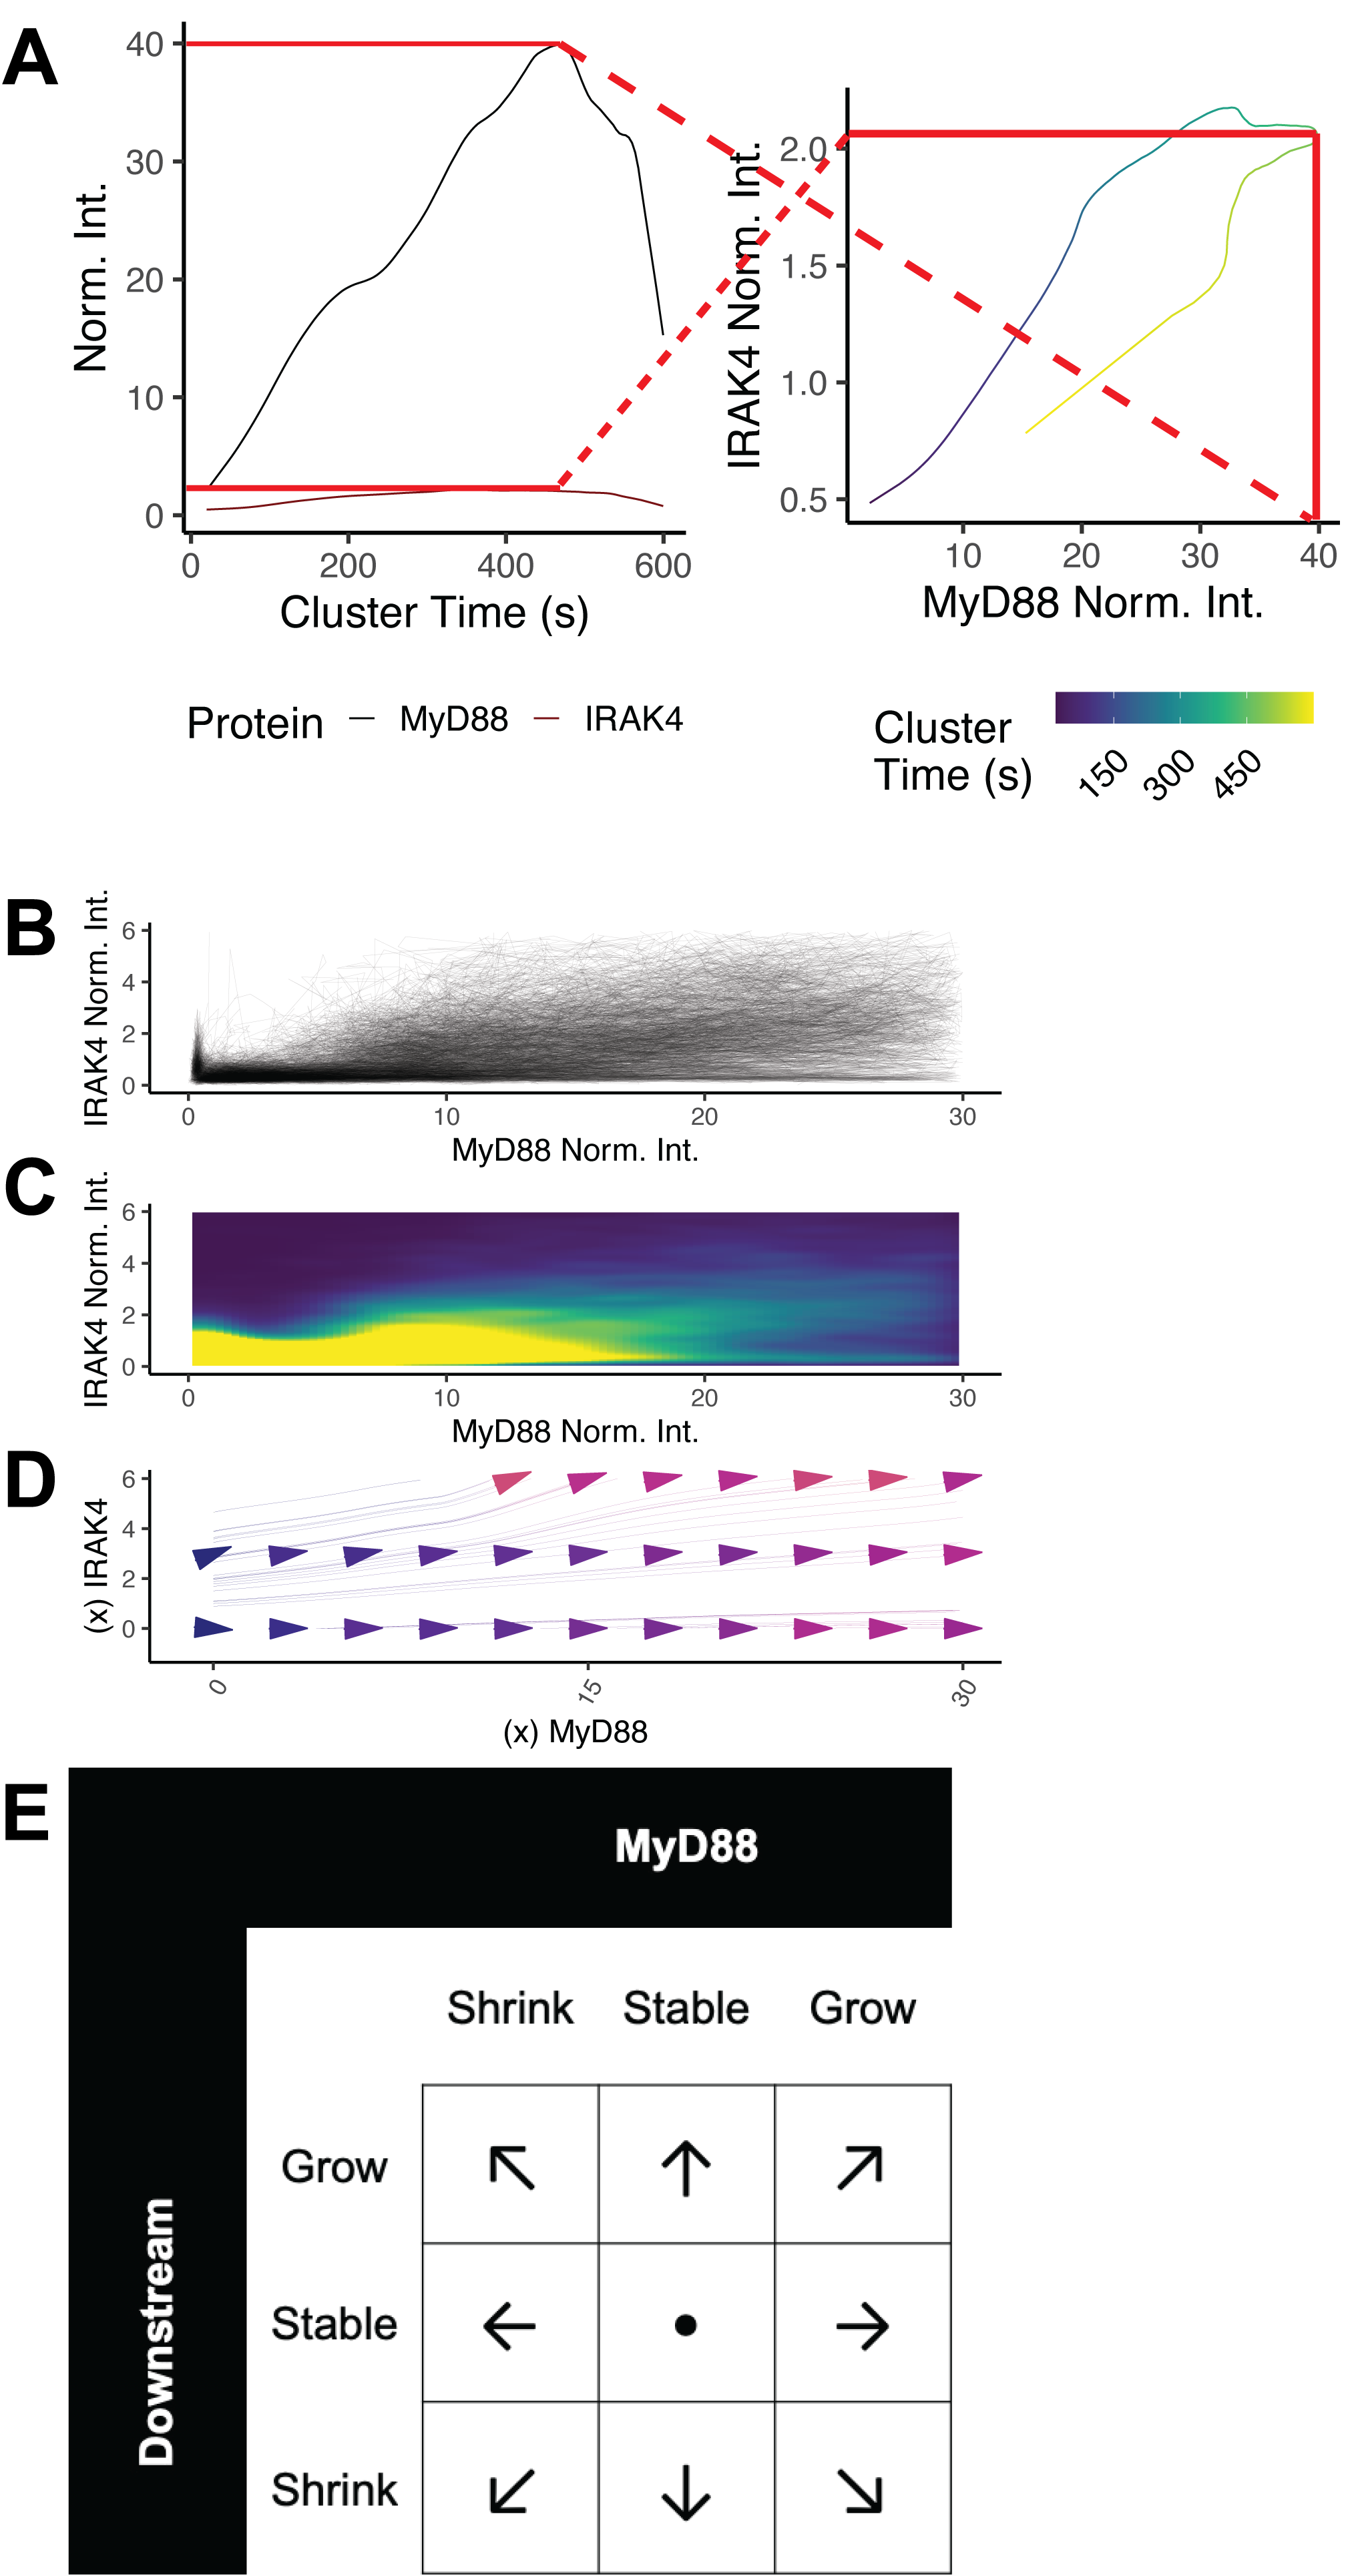
\includegraphics[width=\textwidth, height=\textheight, keepaspectratio]{mod/fig3a.png}}

\captionsetup{parbox=none}
\captionof{figure}[Building and interpreting phase portraits]{\textbf{Building and interpreting phase portraits.} 
\\
\\
(A) Time traces were transformed into phase space, with MyD88 size on the x-axis and downstream protein size on the y-axis. The example shown depicts time through color gradients.
\\
\\
(B) All MyD88-IRAK4 tracks in phase space. Most puncta exhibit MyD88 growth, while some primarily show IRAK4 growth. Only a few recruit both proteins.
\\
\\
(C) Density of tracks in phase space. The farther from the origin (0\times MyD88, 0\times IRAK4), the fewer tracks. To better understand the overall behavior, the data needs to be summarized.
\\
\\
(D) Data in phase space was binned using a step size of three, leading to bins that increase in multiples of three (0\times, 3\times, 6\times, 9\times). The average change in intensity for each bin was calculated using the intensity five frames forward minus five frames backward ($\pm$5 frames, or $\pm$20 seconds). The median intensity change for each bin was plotted as an arrow, with the arrow color indicating the magnitude of growth as an absolute value. To differentiate between growth and disassembly, the arrow angle must be considered.
\\
\\
(E) Arrow angles indicate protein growth or disassembly. A right-pointing arrow signifies MyD88 growth, while an upward arrow indicates downstream protein growth. Conversely, a bottom-left-pointing arrow implies disassembly of both proteins. The arrow angle is calculated using the two-argument tangent (atan2) of the downstream protein and MyD88 change in intensity. Further details on this calculation can be found in Methods~\ref{chapter:PIRATES_PARLEYS}.
\\
\\
(A-D: Imaging data courtesy of Niranjan Srikanth. Analysis, plots by the thesis author.)}
\label{p2:3a}
\end{centering}

The hypothesis was that the phase portraits would initially demonstrate MyD88 growth ($\rightarrow$) for small downstream protein assemblies located at the bottom of the y-axis. This implies an assumption that MyD88 always grows prior to the downstream protein. If downstream proteins have MyD88 size thresholds, then the phase portrait arrows should start rotating, eventually pointing completely upwards. The inflection point would signify the size threshold. Subsequently, I anticipated growth in the downstream protein, indicated by upward-pointing arrows. Considering these proteins likely contain MyD88, these arrows would primarily populate larger MyD88 sizes, that is, they would primarily be located to the right of the x-axis. Upon reaching a stoichiometric ratio high on the y-axis and to the right of the x-axis, I expect these arrows to show minimal growth (small magnitude) because they have reached a state of equilibrium. The events that follow are intriguing since there is no consensus in the field on whether the IL-1 pathway remains stable or disassembles. If the pathway remains stable, the proteins stay put and converge towards a stability point. However, if disassembly occurs, three scenarios are possible: MyD88 disassembles first, the downstream protein disassembles first, or both proteins disassemble together. Alternatively, instead of disassembly, proteins could break apart, moving outside the z-axis of the TIRF microscope’s field of view and into the cytosol.

I plotted the phase portraits (Fig. \ref{p2:3}F-G). Starting with IRAK4, it was noted that in its absence, MyD88 grew (right-pointing arrows when IRAK4 is 0) (Fig. \ref{p2:3}F). However, there were no upward-pointing arrows with no distinguishable inflection point, indicating predominantly IRAK4 growth. Instead, most arrows pointed up-right, suggesting simultaneous growth of MyD88 and IRAK4. One possibility is that once MyD88 binds to the IL-1R, the Myddosome does not distinguish between MyD88 and IRAK4. Another possibility is that the puncta are merging, leading to an increase in the size of both proteins. Still, I would have expected merging to occur only above 6\times MyD88. Even at 3\times MyD88, IRAK4 oligomerization was visible. MyD88 recruits IRAK4 at around 14 seconds (Results~\ref{chapter:p1}; Deliz-Aguirre et al., 2021). Since I computed the change in intensities for 44 seconds ($\pm$5 frames at 0.25 Hz), the temporal resolution may not be high enough to capture such rapid dynamics.

The phase portrait of TRAF6 resembled that of IRAK1, but featured diagonal arrows for all MyD88 assembly sizes at 3\times TRAF6 (Fig. \ref{p2:3}F). This could suggest the absence of a size threshold. However, when MyD88 is large, the growth rate of TRAF6 increases. I also noticed assemblies of MyD88 larger than 15\times that never recruited TRAF6. This phenomenon was not seen in IRAK4 and IRAK1. This could indicate that some Myddosomes do not recruit TRAF6, possibly signaling through another pathway.

The phase portrait of TAB2 mirrors that of TRAF6 in that there appear to be two possible pathways. Note that all trajectories above 3\times TAB2 require at least 9\times MyD88 (Fig. \ref{p2:3}F). This suggests that a MyD88 size threshold might exist before TAB2 can bind.

The phase portrait of NEMO clearly shows a MyD88 size threshold, around 3-6\times MyD88, and also displays an upper boundary at 9\times MyD88. Like TRAF6 and TAB2, some large MyD88 assemblies recruit no downstream protein (Fig. \ref{p2:3}G). NEMO also demonstrates its ability to form large structures. At the upper sizes of NEMO, arrows point downwards, with some pointing down-left, indicating a size limit for NEMO.

The phase portrait of HOIL1 shows MyD88 growth. When MyD88 reaches 24\times, it begins to incorporate HOIL1, and once it reaches 27\times MyD88 3\times HOIL1, the phase portrait shows almost exclusive HOIL1 growth. Then, the arrows point to the left indicating MyD88 disassembly. Since HOIL1 is still growing, this suggests that HOIL1 molecules remain at the plasma membrane. No HOIL1 structures larger than 9\times HOIL1 were observed, implying that both MyD88 and HOIL1 might have maximum assembly sizes, or in other words, assemblies might have defined stoichiometries or maximum sizes. At 12\times MyD88 6\times HOIL1, the arrow points down-left, suggesting HOIL1 might eventually disassemble, although only one arrow indicated this. The HOIL1 phase portrait provides a clear view of new phenomena: negative regulation and MyD88 disassembly.

The phase portrait of A20 resembles that of HOIL1 in that it forms a horizontally flipped c, that is, $\supset$. It also shows a 3\times A20 maximum size. The 0\times MyD88 3\times A20 arrow indicates that both MyD88 and A20 eventually disassemble. This phase portrait demonstrates the ability of my phase portraits to resolve dynamics as small as 3\times molecules with minimal noise (noise would be arrows pointing in random directions).

The phase portraits exhibit multiple trajectories, suggesting that there might be some flexibility regarding the size thresholds (Fig. \ref{p2:3b}A-B). As the assemblies were resolved at a 3\times resolution, it is likely that these multiple trajectories exist, rather than being due to measurement variance.


\begin{centering}
\centering{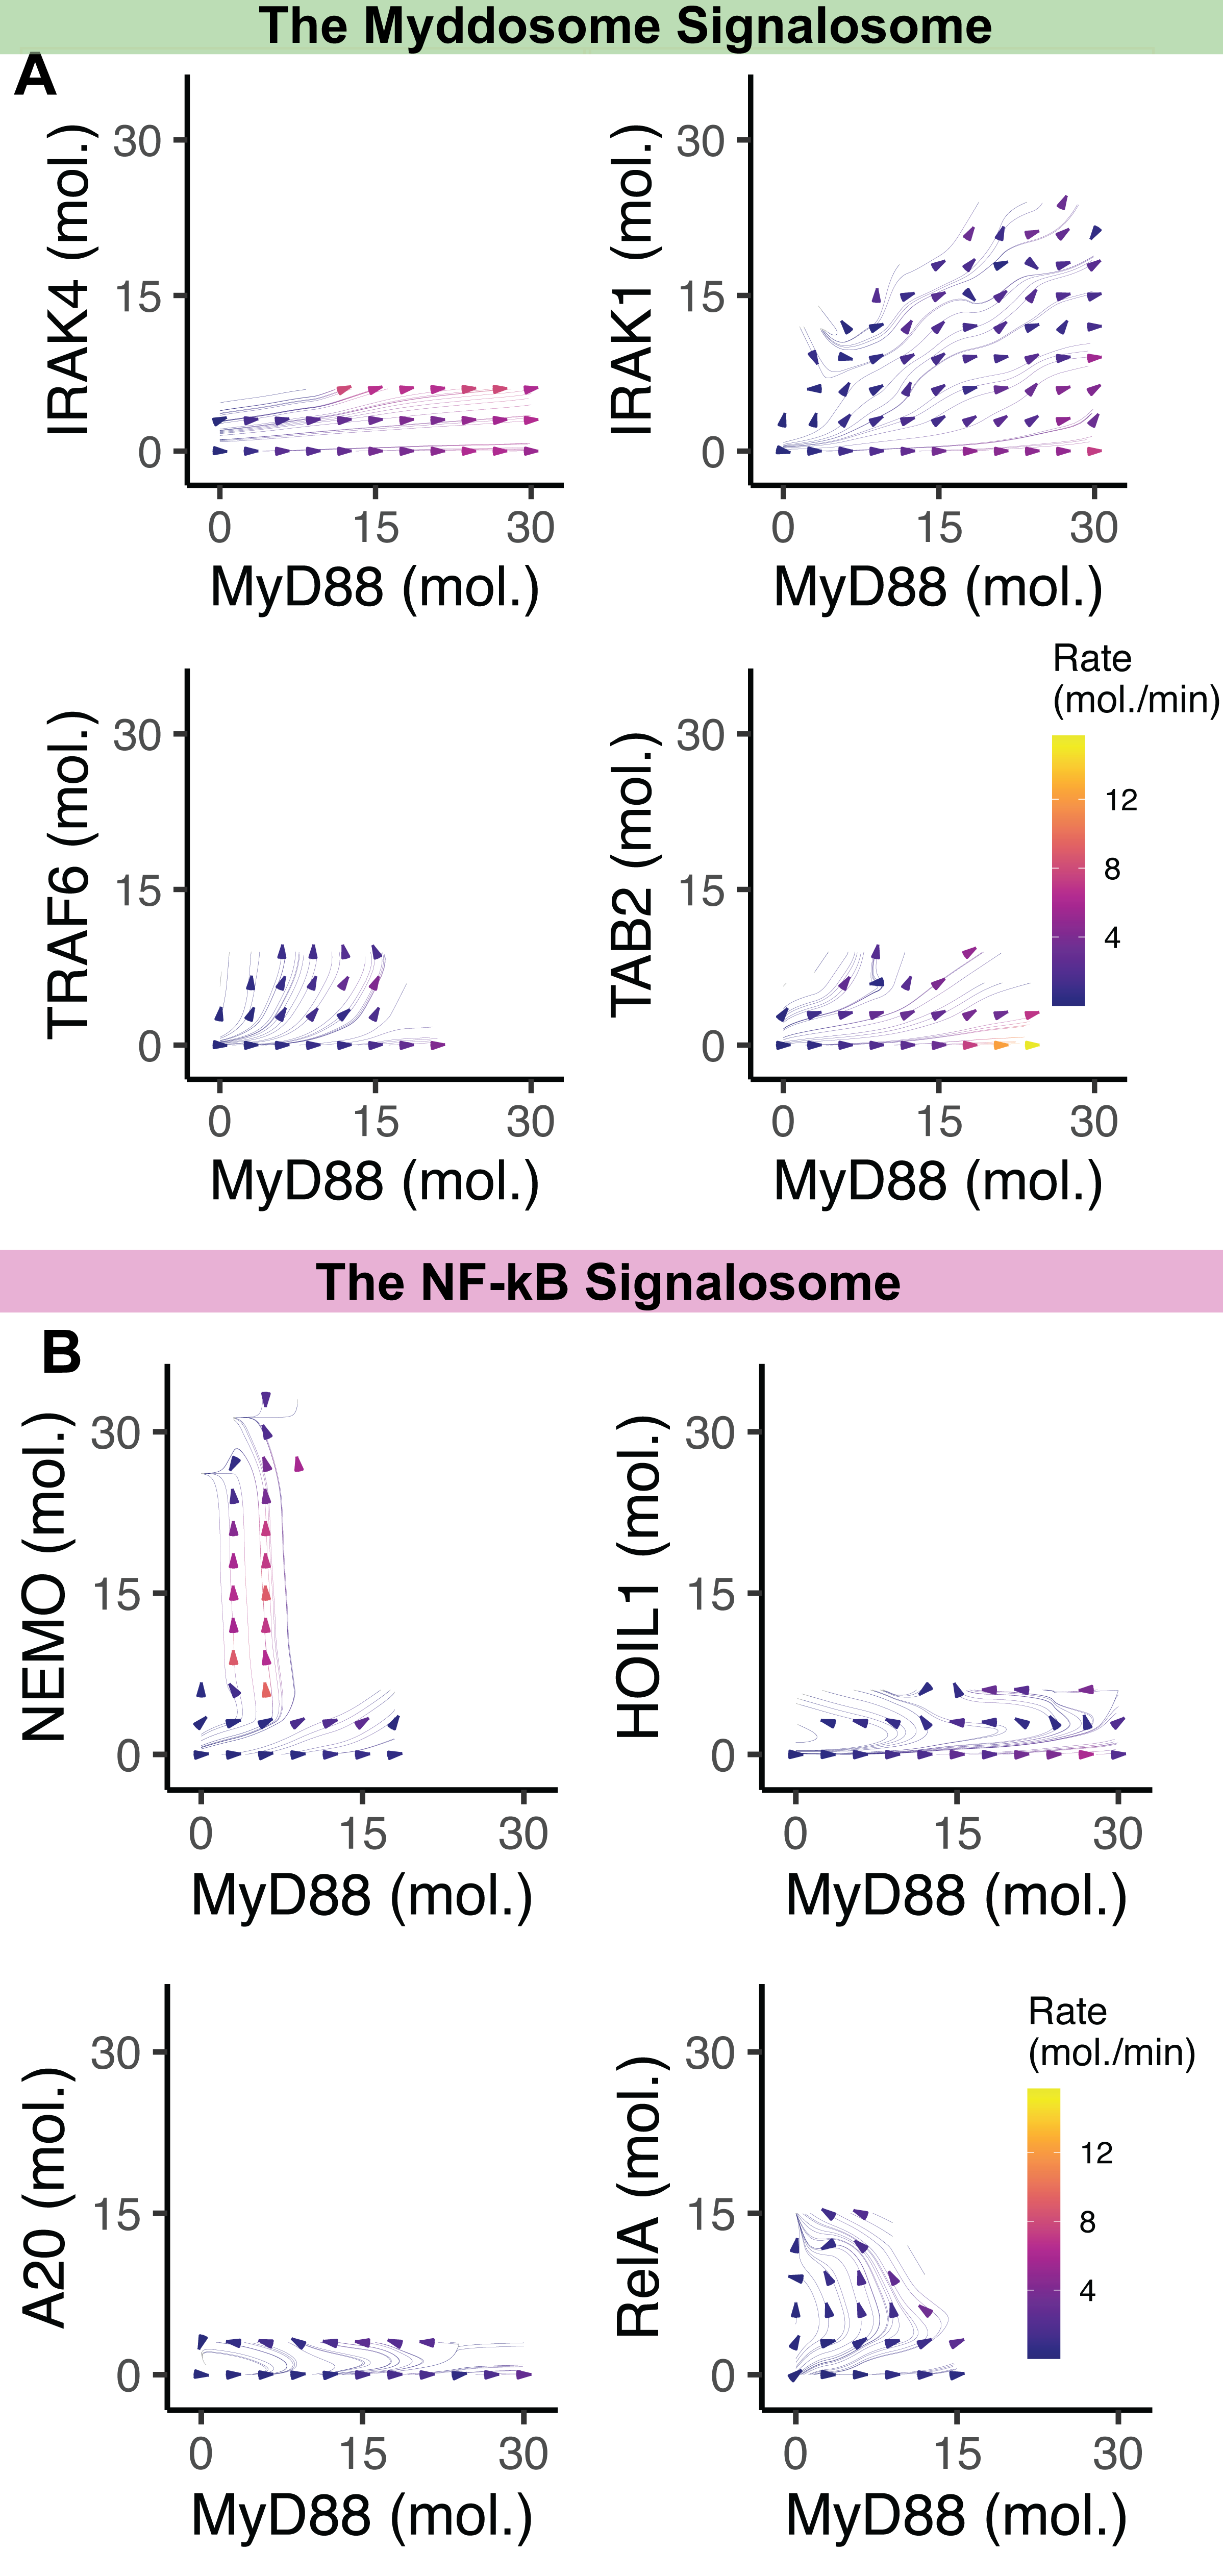
\includegraphics[width=\textwidth, height=\textheight, keepaspectratio]{mod/fig3b.png}}

\captionsetup{parbox=none}
\captionof{figure}[The IL-1 pathway has distinct signalosomes as revealed by phase portrait analysis of MyD88 and downstream protein growth dynamics]{\textbf{The IL-1 pathway has distinct signalosomes as revealed by phase portrait analysis of MyD88 and downstream protein growth dynamics.} 
\\
\\
(A) Phase portraits of IRAK4, IRAK1, TRAF6, and TAB2 display positive feedback with up-right-pointing arrows.
\\
\\
(B) Phase portraits of NEMO, HOIL1, A20, and RelA exhibit a center-like ("circular") pattern, indicating sequential MyD88 growth, downstream protein growth, and ultimately, MyD88 disassembly. This pattern is interpreted as negative feedback.
\\
\\
(A-B) Overall, there are two primary categories of phase portraits: positive and negative feedback. These phase portraits suggest the existence of two signalosomes in the IL-1 pathway: the Myddosome signalosome (positive feedback) and the NF-κB signalosome (negative feedback).
\\
\\
(A-B: Imaging data courtesy of Fakun Cao, Niranjan Srikanth, Elba del Val Oriza and Claudia Abad-Baucells. Analysis, plots by the thesis author.)}
\label{p2:3b}
\end{centering}

I have observed that the MyD88 kinetics show dependency with the downstream protein oligomer length. In some cases, I observe a positive relationship between these two variables, while in others, we see a negative correlation between MyD88 and the downstream protein.

The signalosomes can be distinguished based on time (Fig. \ref{p2:1b}), phase portraits (Fig. \ref{p2:3}), and kinetics (Fig. \ref{p2:S5}). The kinetics indicate that the downstream proteins of the Myddosome signalosome do not trigger disassembly (Fig. \ref{p2:4}A), unlike the NF-κB signalosome (Fig. \ref{p2:4}B). This information is available in the phase portraits, but it is easier to see in phase lines (Fig. \ref{p2:4}C). I can conclude that the Myddosome signalosome shows positive feedback and the NF-κB signalosome shows negative feedback.

\section{The signalosomes have assembly stages}
\sectionmark{Assembly stages}
The presented phase portraits do not narrate the sequence of events; instead, they illustrate how assemblies behave up to 800 seconds after the first punctum makes its appearance. To unravel the sequence of events, I generated multiple phase portraits with different time cutoffs and analyzed the data cumulatively up to said time thresholds (Fig. \ref{p2:S4}A-B). As time passes, I anticipate the disassembly mechanism will become apparent. I also predict the existence of assembly stages dominated by the activity of a single protein, whether it be growth or disassembly. The parameters used in this chapter were determined by my analysis of fluorophores and their bleaching rates (details in Methods~\ref{}). If protein dynamics remain consistent over time, this will verify that I am observing disassembly and not merely the photobleaching of proteins.

With IRAK4, assembly proceeds rapidly initially, but the pace decreases over time. Around the 400-second mark, the assembly process substantially slows down (Fig. \ref{p2:S4}A). The most rapid MyD88 growth occurs at 200 seconds, while when there is more than 3\times IRAK4, IRAK4 assembly is the fastest at 400 seconds. This suggests that MyD88 grows first, followed by IRAK4 (Fig. \ref{p2:S4}A).

The TRAF6 phase portrait remains fairly consistent. It shows how MyD88 growth precedes TRAF6 growth. Around 1000 seconds, MyD88 starts to disassemble, and TRAF6 follows suit after about 1200 seconds. Additionally, around 800 seconds, the TRAF6 dynamics resemble those of the NF-κB signalosome (Fig. \ref{p2:S4}A). This could indicate that TRAF6 forms a bridge between the Myddosome and NF-κB signalosomes, as seen in mid-assembly timepoints (Fig. \ref{p2:1b}, \ref{p2:D1}).

The TAB2 phase portraits display only MyD88 growth at 200 seconds. At 400 seconds, TAB2 begins to be recruited, but these assemblies don't exceed 3\times TAB2. At 600 seconds, it is apparent that larger TAB2 (at least 6\times) mainly forms where there is larger MyD88 (at least 9\times) (Fig. \ref{p2:S4}A).

The phase portraits of MyD88-NEMO reveal that NEMO begins binding after 600 seconds, which also marks the peak of NEMO growth. Although some NEMO presence was noted earlier, it is now evident that NEMO without MyD88 can distinctly be identified as trimers. At 800 seconds, MyD88 starts to disassemble. By 1000 seconds, MyD88 and NEMO disassemble together (Fig. \ref{p2:S4}B).

The HOIL1 phase portraits indicate MyD88 growth up to 400 seconds. At this point, HOIL1 starts to bind and forms the largest HOIL1 assemblies at 600 seconds. While only HOIL1 growth is visible at 400 seconds, at 600 seconds, MyD88 disassembly is also observable. By 800 seconds, down-left arrows suggest that both HOIL1 and MyD88 are disassembling (Fig. \ref{p2:S4}B).

In conclusion, there are multiple distinct stages for each signalosome; the Myddosome signalosome presents two stages (MyD88 followed by downstream growth), while the NF-κB signalosome introduces a third stage (MyD88 reduction).


\begin{centering}
\centering{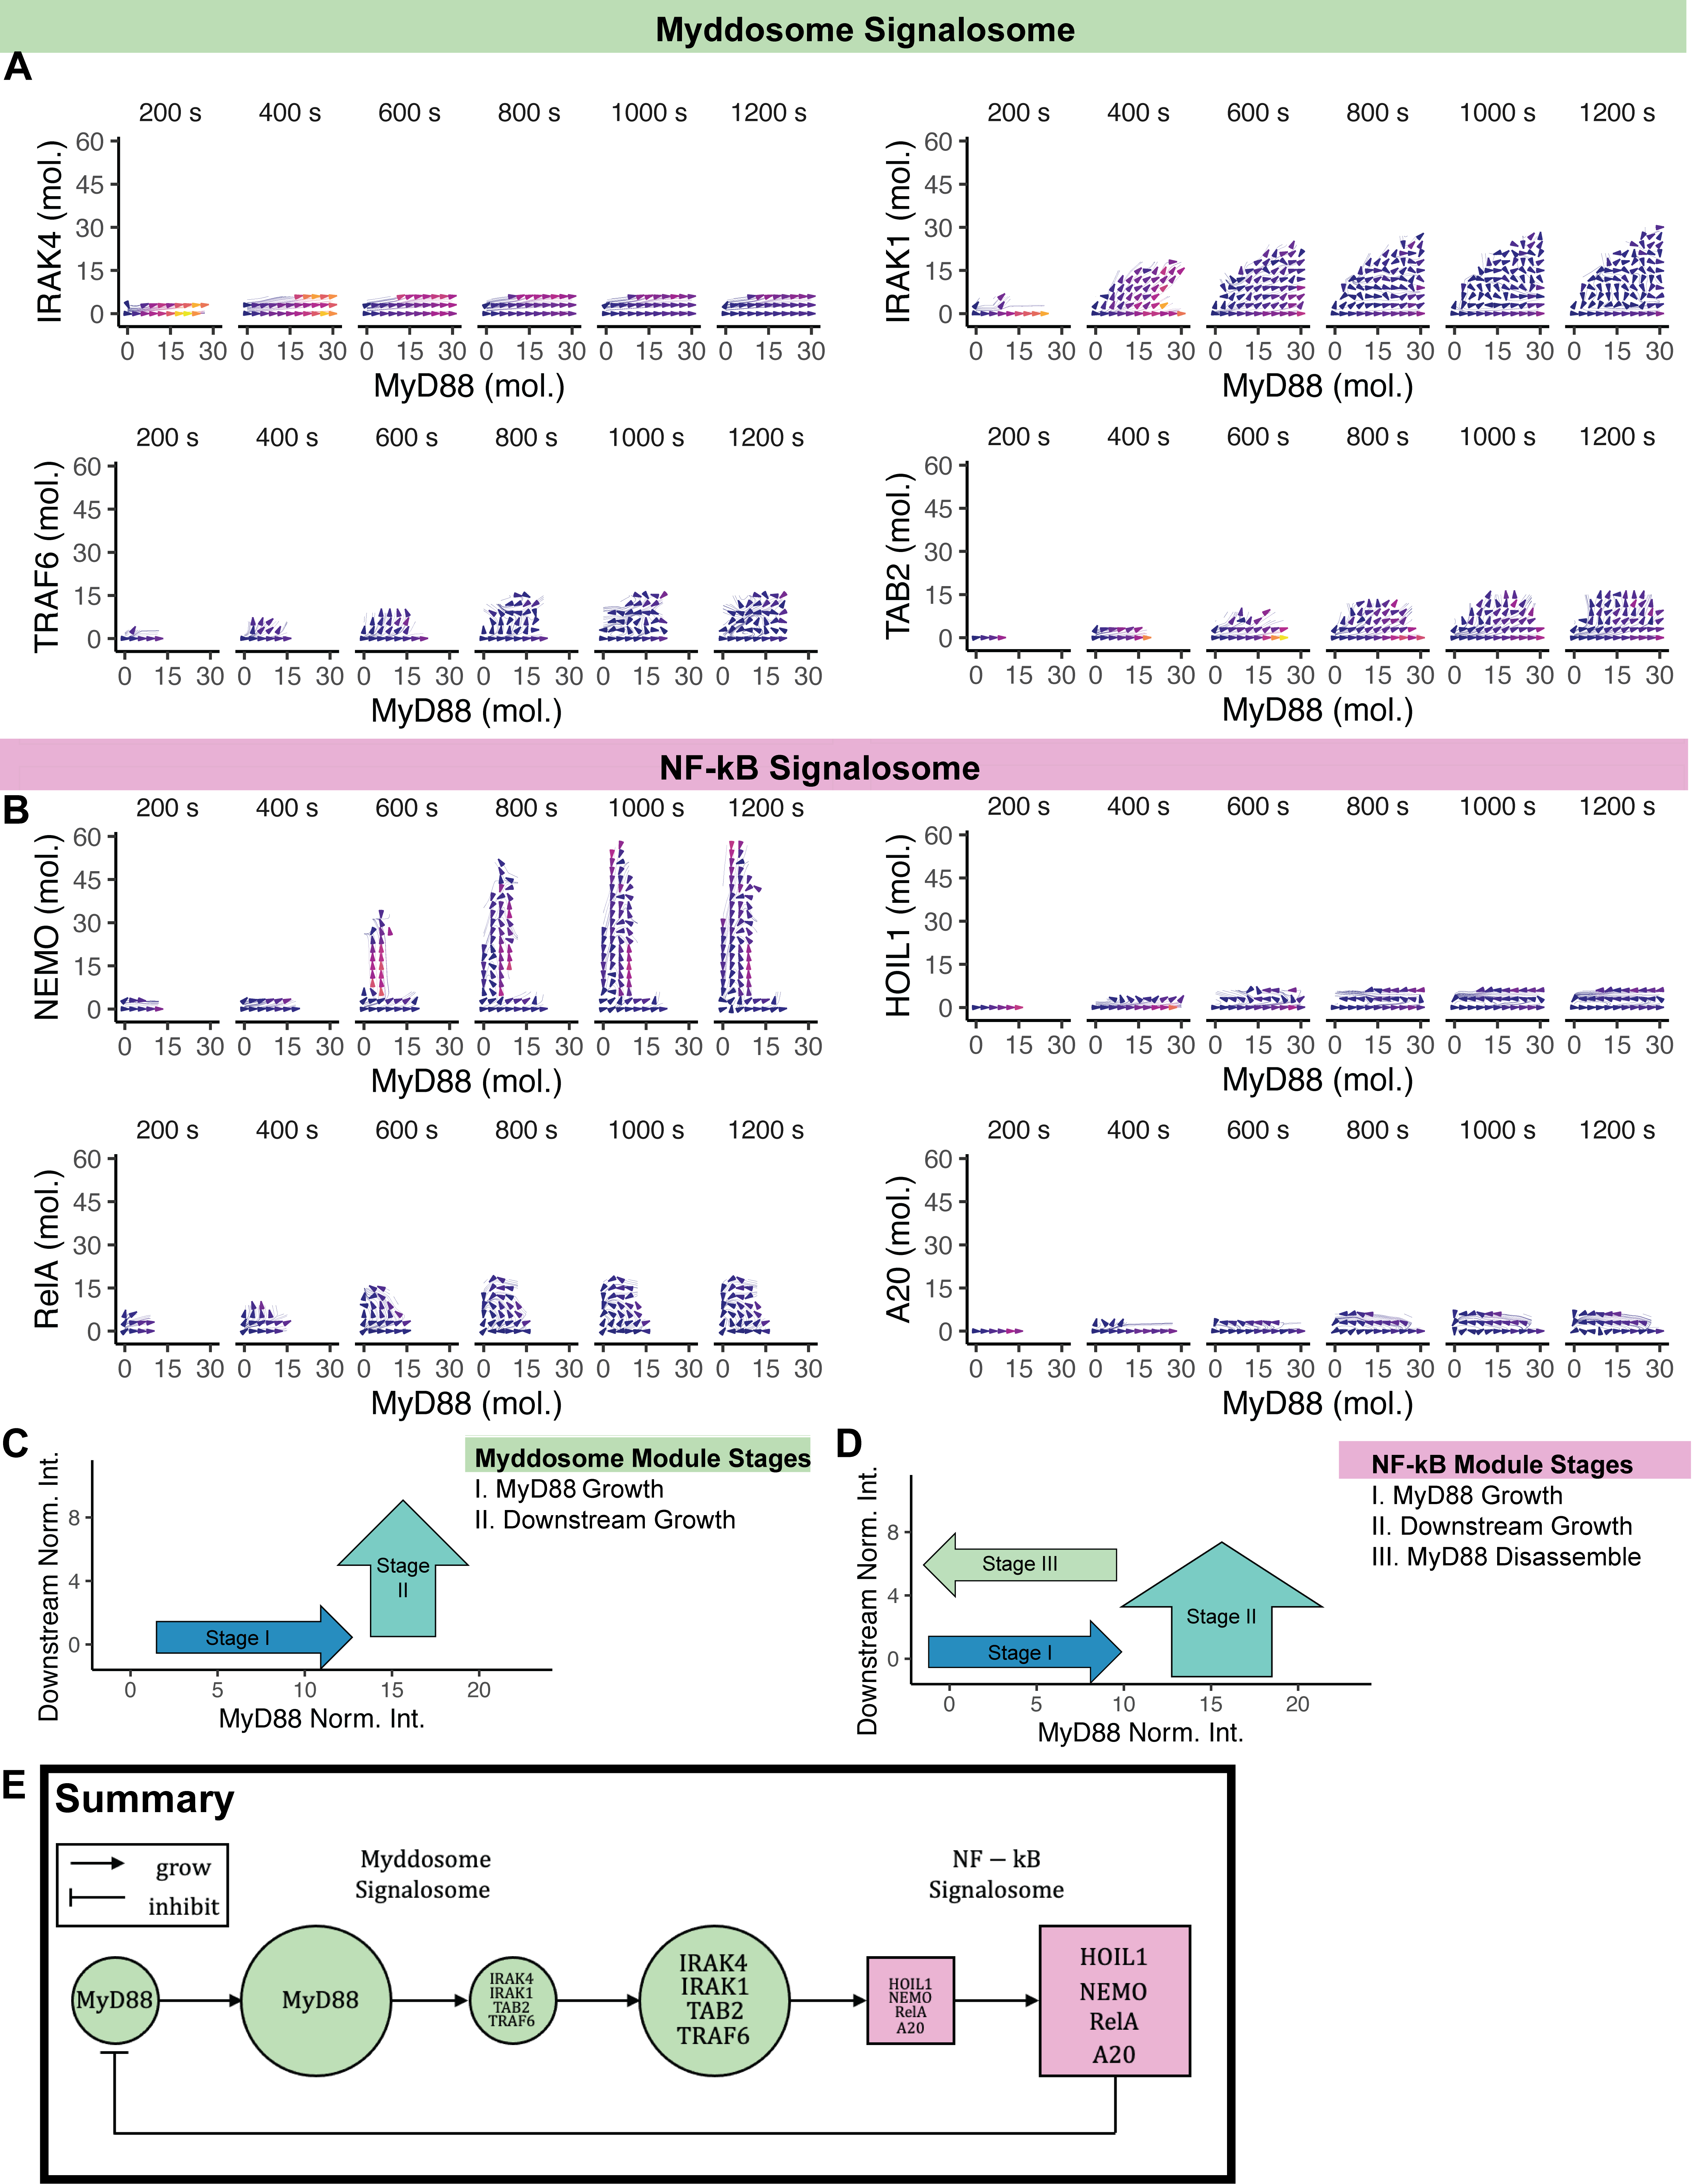
\includegraphics[width=\textwidth, height=\textheight, keepaspectratio]{mod/figS4.png}}

\captionsetup{parbox=none}
\captionof{figure}[IL-1 pathway signalosomes have assembly stages evident in their distinct temporal dynamics]{\textbf{IL-1 pathway signalosomes have assembly stages evident in their distinct temporal dynamics.}
\\
\\
(A-B) Phase portraits with distinct time point cutoffs (facets), with each time point indicating the time elapsed since the appearance of the first spot.
\\
\\
(A) The Myddosome signalosome forms within the initial 400 seconds, suggesting the early formation of the Myddosome module. Based on the populated regions in the phase portrait, the assembly order is IRAK4, IRAK1, TRAF6, and finally, TAB2.
\\
\\
(B) The NF-κB signalosome forms later, around 600 seconds, with MyD88 binding first followed by the recruitment of HOIL1, NEMO, RelA, and ultimately, A20. The NEMO phase portraits indicate that not all large MyD88 assemblies recruit NEMO, suggesting potential binding to a different pathway.
\\
\\
(C-D) Phase portraits can be employed to identify stages in protein assembly.
\\
\\
(C) The Myddosome signalosome displays initial MyD88 growth (right-pointing arrows, 200 seconds) and subsequent recruitment of Myddosome signalosome downstream proteins (IRAK4, IRAK1, TRAF6, TAB2) (upward-pointing arrows, 400 seconds).
\\
\\
(D) The NF-κB signalosome (NEMO, HOIL1, RelA, A20) exhibits similar dynamics of MyD88 assembly (right-pointing arrows), and downstream protein assembly (upward-pointing arrows) but also demonstrates MyD88 disassembly (left-pointing arrows, 800 seconds).
\\
\\
(E) The phase portrait analysis revealed that there are assembly steps where assemblies grow larger over time. Larger Myddosome signalosome assemblies then recruit the NF-κB signalosome. The appearance of the NF-κB signalosome triggers the disassembly of MyD88.
\\
\\
(A-B: Imaging data courtesy of Fakun Cao, Niranjan Srikanth, Elba del Val Oriza and Claudia Abad-Baucells. Analysis, plots by the thesis author.)}
\label{p2:S4}
\end{centering}

\section{The module kinetics are different from each other but similar within}
\sectionmark{Module kinetics}
The phase portraits provide insights into the interaction between two proteins. Alternatively, one could visualize each component individually, using graphical representations known as phase lines (also referred to as 1D phase portraits). Phase lines allow for the visualization of individual protein growth and disassembly in relation to various protein sizes. By multiplying the magnitude by the sine or cosine of the angle, average kinetics of a protein at a specific stoichiometry can be determined. To simplify information, I synthesized the data into two phase lines per plot, using color coding for differentiating with or without a specific protein.

I studied MyD88 kinetics, plotting MyD88 size on the x-axis, MyD88 growth rate on the y-axis, and the presence of small or large downstream proteins (cutoff: 3\times downstream protein) in color. To compute the MyD88 growth rate, I multiplied the cosine of the angle by the magnitude (as illustrated in Fig. \ref{p2:S5}A).

MyD88 growth was the most rapid when there were small downstream protein assemblies present (Fig. \ref{p2:S5}B). The larger the MyD88 assembly, the faster the growth, following a linear trend. The Myddosome signalosome demonstrated positive MyD88 growth even when the downstream protein was present (Fig. \ref{p2:S5}B, blue curves). However, the introduction of IRAK1 and TAB2 slowed down MyD88 growth. Despite a significant reduction in MyD88 growth once these Myddosome signalosome downstream proteins bind, the linear trend persisted, except in the case of IRAK4.

The NF-κB signalosome (Fig. \ref{p2:S5}B, bottom four rows of plots) demonstrated that MyD88 grows with small NF-κB signalosome proteins (NEMO, HOIL1, A20 and RelA). When these proteins bind, MyD88 disassembles (Fig. \ref{p2:S5}B, blue curve with negative numbers on the y-axis), with the disassembly rate increasing for larger MyD88 assemblies. This suggests that MyD88 disassembly is catastrophic-like, quickly disassembling until reaching the x-intercept, 0\times MyD88.

Larger MyD88 Bifurcation, in the realm of dynamical systems, implies the splitting of a system into two distinct trajectories. This phenomenon arises in bistable systems, which possess two equilibrium points. In biochemical terms, we can envision a switch with two potential states. This bifurcation mechanism plays a key role in several biological pathways, such as glycolysis, MAPK/ERK, and hemoglobin, introducing regulatory complexity into the system (Jacobsen \& Trane, 2010; Shiraishi et al., 2010).

My hypothesis suggests that our system's stoichiometries could bifurcate into two distinct assembly categories, potentially due to the existence of multiple stable stoichiometries and varied assembly mechanisms. I predict two distinct assembly trajectories: one beginning with the growth of MyD88, and the other led by the downstream protein. To investigate this conjecture, I analyzed our microscope data.

In examining multiple cell lines, I discerned two types of assembly dynamics: one where MyD88 reaches mid-intensity first, and another where the downstream protein takes the lead, as observed in the MyD88-TRAF6 cell line (Fig. \ref{p3:1}A). This observation substantiates my hypothesis but does not provide information regarding the frequency of these dynamics. It raises questions about whether proteins consistently maintain the same stoichiometric ratios from initiation to completion. To address this, I performed a 2D density plot comparing the starting and ending stoichiometries, using the percentage of MyD88 as a ratio.

Generally, most puncta maintain the same stoichiometry from start to end (depicted by the diagonal line), with exceptions being IRAK1, TRAF6, NEMO, TAB2, and RelA, where some puncta deviate from the diagonal line (Fig. \ref{p3:1}C). This shift in ratio indicates potential candidates for bifurcation. Yet, it doesn't provide insight into the underlying mechanism of this shift. To explore whether proteins transition between assembly trajectories and understand how different proteins enrich the assemblies, I created phase portraits of the stoichiometric ratios (percentage of MyD88 in the puncta) over time, with frequency colorized and arrow angle indicating the growth direction.

Analysis of the stoichiometry phase portraits reveals that usually, MyD88 growth precedes the joining of the downstream protein. Notably, IRAK1, TRAF6, NEMO, TAB2, and RelA data bifurcate around the 40-second mark of puncta time. In the case of the MyD88-IRAK1 cell line, assemblies richer in IRAK1 tend to abort earlier, while those richer in MyD88 appear more stable, a pattern that is consistent with TRAF6 and TAB2. Interestingly, for NEMO and RelA, we observe a bistable system, where both MyD88-rich and NEMO/RelA-rich assemblies persist for similar durations. The best predictor of the final stoichiometric ratio is the initial stoichiometric ratio (Fig. \ref{p3:1}D), suggesting that the assembly of the IL-1 pathway is deterministic in nature.
 contain more downstream protein, suggesting a direct relationship between the two (Fig. \ref{p2:S1}-\ref{p2:S2}). Therefore, a negative rate constant exists between the MyD88 kinetics and the downstream protein assembly size.

The evidence indicates that these NF-κB signalosome proteins induce a rapid, catastrophic-like disassembly, resulting in a swift collapse of MyD88, comparable to the complete breakdown of the cytoskeleton.

Continuing with the analysis of MyD88 kinetics, I plotted the downstream (D/S) protein size on the x-axis, the MyD88 growth rate on the y-axis, and distinguished between small or large MyD88 assemblies (cutoff: 3\times downstream protein) using color. To calculate the MyD88 growth rate, I multiplied the cosine of the angle by the magnitude (Fig. \ref{p2:S5}C illustrates this process).

When there is less than 3\times MyD88, the growth of MyD88 is slow (Fig. \ref{p2:S5}D, red curve). IRAK4 appears to synergistically promote MyD88 growth, as an increase in IRAK4 enhances MyD88 growth (Fig. \ref{p2:S5}D, blue curves). The remaining Myddosome signalosome proteins display a consistent MyD88 growth rate, regardless of the downstream protein size in the complex.

For HOIL1 and A20 of the NF-κB signalosome (Fig. \ref{p2:S5}D), the presence of more downstream protein leads to a faster MyD88 disassembly when there is at least 3\times MyD88 in the assembly. This suggests a negative constant that impacts MyD88 growth based on the size of HOIL1 and A20. This pattern also occurs with RelA, although to a lesser extent.

Next, I examined the downstream protein kinetics, plotting MyD88 size on the x-axis, downstream protein growth rate on the y-axis, and distinguishing between small or large downstream protein assemblies (cutoff: 3\times downstream protein) using color. To derive the downstream protein growth rate, I multiplied the sine of the angle by the magnitude (Fig. \ref{p2:S5}E illustrates this process).

In all cases, the downstream protein growth rate is negligible, irrespective of MyD88 size, provided the downstream protein size is small (Fig. \ref{p2:S5}F, red curves).

When the downstream protein size exceeds 3\times, growth is observed in IRAK4, TAB2, and RelA, while IRAK1, HOIL1, and A20 primarily disassemble. The sigmoidal shape of IRAK4, TAB2, and RelA suggests cooperativity, although the trend is not entirely clear. Additionally, these phase lines do not show the downstream protein disassembling.

The NEMO growth rate as a function of MyD88 size in the presence of NEMO displays an intriguing curve that appears both sigmoidal and step-like. The initial phase shows rapid disassembly, suggesting that MyD88 is repelling NEMO, probably due to MyD88 instability and its inability to bind NEMO. Then, at 6-9\times MyD88, there is no NEMO growth. This switch-like behavior indicates a transition point. The end of the curve shows rapid assembly, implying that larger MyD88 assemblies are stable and can bind NEMO. This could be modeled by considering a dissociation constant and a binding constant. For small MyD88 assemblies, NEMO disassociation is stronger than NEMO binding. At 6-9\times MyD88, the constants balance each other out. As MyD88 grows, it stabilizes, and the NEMO binding rate exceeds the NEMO dissociation rate.

Finally, I investigated the downstream protein kinetics, but this time, I plotted the downstream protein size on the x-axis, the MyD88 growth rate on the y-axis, and differentiated between small or large MyD88 assemblies (cutoff: 3\times MyD88) using color. To derive the downstream protein growth rate, I multiplied the sine of the angle by the magnitude (Fig. \ref{p2:S5}G illustrates this process).

With few or no MyD88 (Fig. \ref{p2:S5}H, 0-3\times MyD88, red curves), most downstream proteins exhibit no growth. Downstream proteins require a MyD88 size threshold before they can colocalize with MyD88 (Fig. \ref{p2:3}). Therefore, it is plausible that the absence of growth is due to a lack of downstream proteins.

NEMO disassembles proportionally to its size, even without MyD88. This supports the previous observation that small (0-3\times) MyD88 assemblies strongly repel large NEMO assemblies. An alternate explanation could be that these points mark the end of assembly, and what I'm observing is the dissociation of NEMO. This could occur because there is no MyD88 to stabilize NEMO, or because the assembly has catastrophically collapsed, leading to the dissociation of all proteins.

In the presence of MyD88, TAB2, NEMO, A20, and RelA grow, exhibiting positive growth trends relative to MyD88 (Fig. \ref{p2:S5}H, blue curves). More specifically, these proteins suggest cooperative binding because their kinetic curves are sigmoidal, featuring slow early assembly that progressively accelerates until reaching a plateau. The data also implies that TAB2, NEMO, A20, and RelA require a MyD88 size threshold to be reached before these proteins can grow. This conclusion is drawn from the red curves with less than 3\times MyD88 (Fig. \ref{p2:S5}H). Without MyD88, there's no growth of TAB2, A20, and RelA. These proteins also demonstrate a plateau in their growth rates, with the sigmoidal shape indicating that at low downstream protein sizes, the affinity is low. As more downstream proteins bind, the affinity increases until it reaches a saturation point where binding cannot occur any faster.

The plots demonstrate that different signalosomes exhibit different kinetics. The Myddosome signalosome shows positive growth trends among its proteins, while the proteins in the NF-κB module display a negative relation to MyD88. NEMO, in particular, provided insightful data. Its kinetic data suggested that downstream proteins might have dissociation constants in conflict with binding constants, manifesting as a MyD88 size threshold that needs to be crossed for successful downstream protein binding. Although most trends were linear, some curves displayed switch-like, sigmoidal, or plateauing behavior, indicating that the IL-1 pathway is a complex system exhibiting non-linearity (explained further in Methods~\ref{section:complex}). This nonlinearity can introduce dynamics beneficial to a biological signaling network.

From an engineering perspective, non-linearity can introduce control. For instance, non-linearity can amplify signals in biological circuits, thereby enhancing sensitivity. T-cell ligand discrimination is believed to operate in this manner (McKeithan, 1995). Non-linearity can also generate switch-like and oscillatory behaviors in signaling (DeFelice et al., 2019).


\begin{centering}
\centering{\includegraphics[width=\textwidth, height=\textheight, keepaspectratio]{mod/figS5.png}}

\captionsetup{parbox=none}
\captionof{figure}[One-dimensional phase portraits reveal feedback and trends in the assembly and disassembly kinetics of the Myddosome and NF-κB signalosomes]{\textbf{One-dimensional phase portraits reveal feedback and trends in the assembly and disassembly kinetics of the Myddosome and NF-κB signalosomes.} One-dimensional (1D) phase portraits illustrating pathway dynamics. On the top are explanations of how these 1D phase portraits were constructed, and on the right are the results. The top row of plots with the green background represents the Myddosome signalosome, while the bottom row with the magenta background represents the NF-κB signalosome. Protein order remains the same, but arranged from top to bottom.
\\
\\
(A) MyD88 size is in the x-axis, MyD88 growth/disassembly in the y-axis calculated using the following formula, $\Delta\text{MyD88} = \cos(\theta) \times |\text{magnitude}|$, and in color is the curve which indicates kinetics for small (red, <3\times) or large (blue, $\geq$3\times) downstream protein (D/S prot.) assemblies.
\\
\\
(B) In the absence of the downstream protein, a linear trend between MyD88 size and growth is observed (red curves), with larger MyD88 puncta promoting faster growth. This relationship is linear, with MyD88 size and growth rate being proportional. The Myddosome signalosome (top four rows in green) exhibits positive MyD88 growth, even in the presence of the downstream protein (blue curve). However, the presence of IRAK1 and TAB2 (Myddosome signalosome proteins) slow down MyD88 growth. MyD88 growth is significantly reduced once these downstream proteins bind, but the linear trend between MyD88 size and growth is still present, except for IRAK4.
\\
\\
The NF-κB signalosome (bottom four rows in magenta) shows that, in the absence of NEMO, HOIL1, A20, and RelA, MyD88 grows. When these proteins are present (blue curve), MyD88 disassembles (negative numbers on the y-axis), with the disassembly rate increasing (quicker disassembly) for larger MyD88 assemblies. Larger MyD88 assemblies have more downstream protein, as there is a direct relationship between the two, as shown in earlier plots in this chapter. This means that these downstream proteins trigger a rapid, catastrophic-like disassembly in which MyD88 collapses quickly.
\\
\\
(C) Downstream size is in the x-axis, MyD88 growth/disassembly in the y-axis calculated using the following formula, $\Delta\text{D/S} = \cos(\theta) \times |\text{magnitude}|$, and in color is the curve which indicates kinetics for small (red, <3\times) or large (blue, $\geq$3\times) MyD88 assemblies.
\\
\\
(D) In all cases, MyD88 growth is slow when there is less than 3\times MyD88 (red curve). IRAK4 promotes MyD88 growth synergistically, as more IRAK4 enhances MyD88 growth. The rest of the Myddosome signalosome proteins show a constant MyD88 growth rate, regardless of the downstream protein size in the complex. In IRAK4, MyD88 grows faster when there is more than 3\times MyD88 (blue curves).
\\
\\
For HOIL1 and A20 of the NF-κB signalosome (bottom rows in magenta), the more downstream protein there is, the faster MyD88 disassembles when there is at least 3\times MyD88 in the assembly. This means there is a negative trend between MyD88 growth and the size of HOIL1 and A20.
\\
\\
(E) MyD88 size is in the x-axis, downstream protein growth/disassembly in the y-axis calculated using the following formula, $\Delta\text{Downstream Protein} = \sin(\theta) \times |\text{magnitude}|$, and in color is the curve which indicates kinetics for small (red, <3\times) or large (blue, $\geq$3\times) downstream protein assemblies.
\\
\\
(F) For each MyD88 size (x-axis), the growth rate of the downstream protein (y-axis) was examined in the presence (blue) or absence (red) of the downstream protein. For all cases, the downstream protein growth rate is negligible, regardless of MyD88 size, when the downstream protein size is small (red curves).
\\
\\
When the downstream protein size exceeds 3\times, growth is observed in IRAK4, TAB2, and RelA, whereas IRAK1, HOIL1, and A20 primarily disassemble. NEMO disassembles with up to 3\times MyD88 but grows with 9\times MyD88, possibly due to the overall disassembly observed in the phase portraits. This implies that small MyD88 assemblies strongly repel large ($\geq$3\times) NEMO assemblies, whereas large ($\geq$12\times) MyD88 assemblies promote NEMO oligomerization. Between 6-9\times MyD88, the effects of growth and disassembly offset each other in the 1D phase portrait, but with a slight preference for growth.
\\
\\
(G) Downstream protein size is in the x-axis, downstream protein growth/disassembly in the y-axis calculated using the following formula, $\Delta\text{Downstream Protein} = \sin(\theta) \times |\text{magnitude}|$, and in color is the curve which indicates kinetics for small (red, <3\times) or large (blue, $\geq$3\times) MyD88 assemblies.
\\
\\
(H) In the absence of MyD88 (<3\times MyD88, red curves), most proteins show no growth, likely because there is no downstream protein present. Downstream proteins have a MyD88 size threshold before they colocalize with MyD88, as demonstrated in earlier plots. NEMO disassembles proportional to its size, even without MyD88. This supports the previous observation that small (<3\times) MyD88 assemblies strongly repel large NEMO assemblies.
\\
\\
In the presence of MyD88, TAB2, NEMO, A20, and RelA grow, exhibiting positive trends in their growth relative to MyD88 (blue curves). However, the data also suggest that TAB2, NEMO, A20, and RelA have MyD88 size thresholds that must be met before these proteins grow. These proteins also exhibit a plateau in their growth rates, with the sigmoidal shape indicating that at low downstream protein sizes, the affinity is low. As more downstream proteins bind, the affinity increases until it reaches a saturation point where binding cannot occur any faster.
\\
\\
Dot size indicates N, points are medians, the spread is the standard error of the median.
\\
\\
(A-H: Imaging data courtesy of Fakun Cao, Niranjan Srikanth, Elba del Val Oriza and Claudia Abad-Baucells. Analysis, plots by the thesis author.)}
\label{p2:S5}
\end{centering}

\section{A modified Lotka-Volterra equation fits TRAF6-NEMO phase portraits}
\sectionmark{Disassembly}
Below are the equation parameters and fitted values of the modified Lotka-Volterra.

\begin{equation}
\begin{aligned}
\frac{dx}{dt} &= \alpha x - \beta xy \\
\frac{dy}{dt} &= \delta xy -\gamma y - \epsilon y^2 
\end{aligned}
\end{equation}
Where
\begin{equation}
\begin{aligned}
\frac{dx}{dt} &= \text{TRAF6 growth rate} \\
\frac{dy}{dt} &= \text{NEMO growth rate} \\
\\
x &= \text{TRAF6 size} \\
y &= \text{NEMO size} \\
t &= \text{time} \\
\alpha & = \text{TRAF6 growth rate} \\
\beta & = \text{TRAF6-NEMO binding rate} \\
\gamma & = \text{NEMO disassembly rate} \\
\delta & = \text{cooperativity coefficient} \\
\epsilon & = \text{regulation/inhibition rate}
\end{aligned}
\end{equation}

\begin{equation}
\begin{aligned}
\alpha &= 2.26\times 10^{-3} \text{ mol.} \text{s}^-\\
\beta &= 0.11\times 10^{-3} \text{ }(\text{mol.}\times \text{s})^-\\
\gamma &= -1.22\times 10^{-3} \text{ s}^-\\
\delta &= 0.66\times 10^{-3} \text{ } (\text{mol.}\times \text{s})^-\\ 
\epsilon &= 0.24\times 10^{-3} \text{ } (\text{mol.}\times \text{s})^- 
\end{aligned}
\end{equation}
The phase portrait using these parameters is shown in Fig. \ref{p2:6a}A. Based on these parameters, the TRAF6 ($x$) solution is:
\begin{equation}
x = A e^{\alpha t - \beta \frac{y^2}{2}}
\end{equation}
Where $A$ is the starting point. Which is a population growth model, but with an additional parameter, $\beta \frac{y^2}{2}$. Thus, it could loosely be interpreted as a logistic growth model. This means that there is an upper boundary to the TRAF6 protein size in the assembly. In other words, there is a TRAF6 carrying capacity in the assembly. The NEMO solution is:
\begin{align*}
\frac{1}{y(\delta e^{\alpha t - \beta\frac{y^2}{2} + C_1} - \gamma - \epsilon y)}dy &= dt \\
\int \frac{1}{y(\delta e^{\alpha t - \beta\frac{y^2}{2} + C_1} - \gamma - \epsilon y)}dy &= \int dt
\end{align*}
Which cannot be solved analytically, but it can be solved numerically. For this system, the equilibrium points are 0\times TRAF6 0\times NEMO and 37\times TRAF6 24\times NEMO, both which are stable nodes for this spiral phase portrait.

\section{The Myddosome and NF-κB signalosomes have a carrying capacity}
\sectionmark{Carrying capacity}
In comparing the experimental data with the theoretical predator-prey models, including Holling-Tanner, Gause, and Leslie-Gower, I can see that these models fit some of the trends, but do not fully capture the shape of the phase portraits nor the behavior observed in the data. The unmodified Holling-Tanner model produced a respectable correlation (R = 0.72) with the experimental data, yet it failed to accurately recreate the shape of the phase portraits, demonstrating an area of disconnect between the theoretical model and the experimental results.

To overcome this limitation, I adapted these models by incorporating a logistic growth parameter in the form of a polynomial (Methods~\ref{chapter:differential_equations}, Fig. \ref{p2:S6}C). This modification served to increase the resemblance of the theoretical models to the experimental data. The modified Lotka-Volterra model, in particular, provided a better fit (R = 0.85), highlighting the importance of accounting for the logistic growth in our analysis.



\begin{centering}
\centering{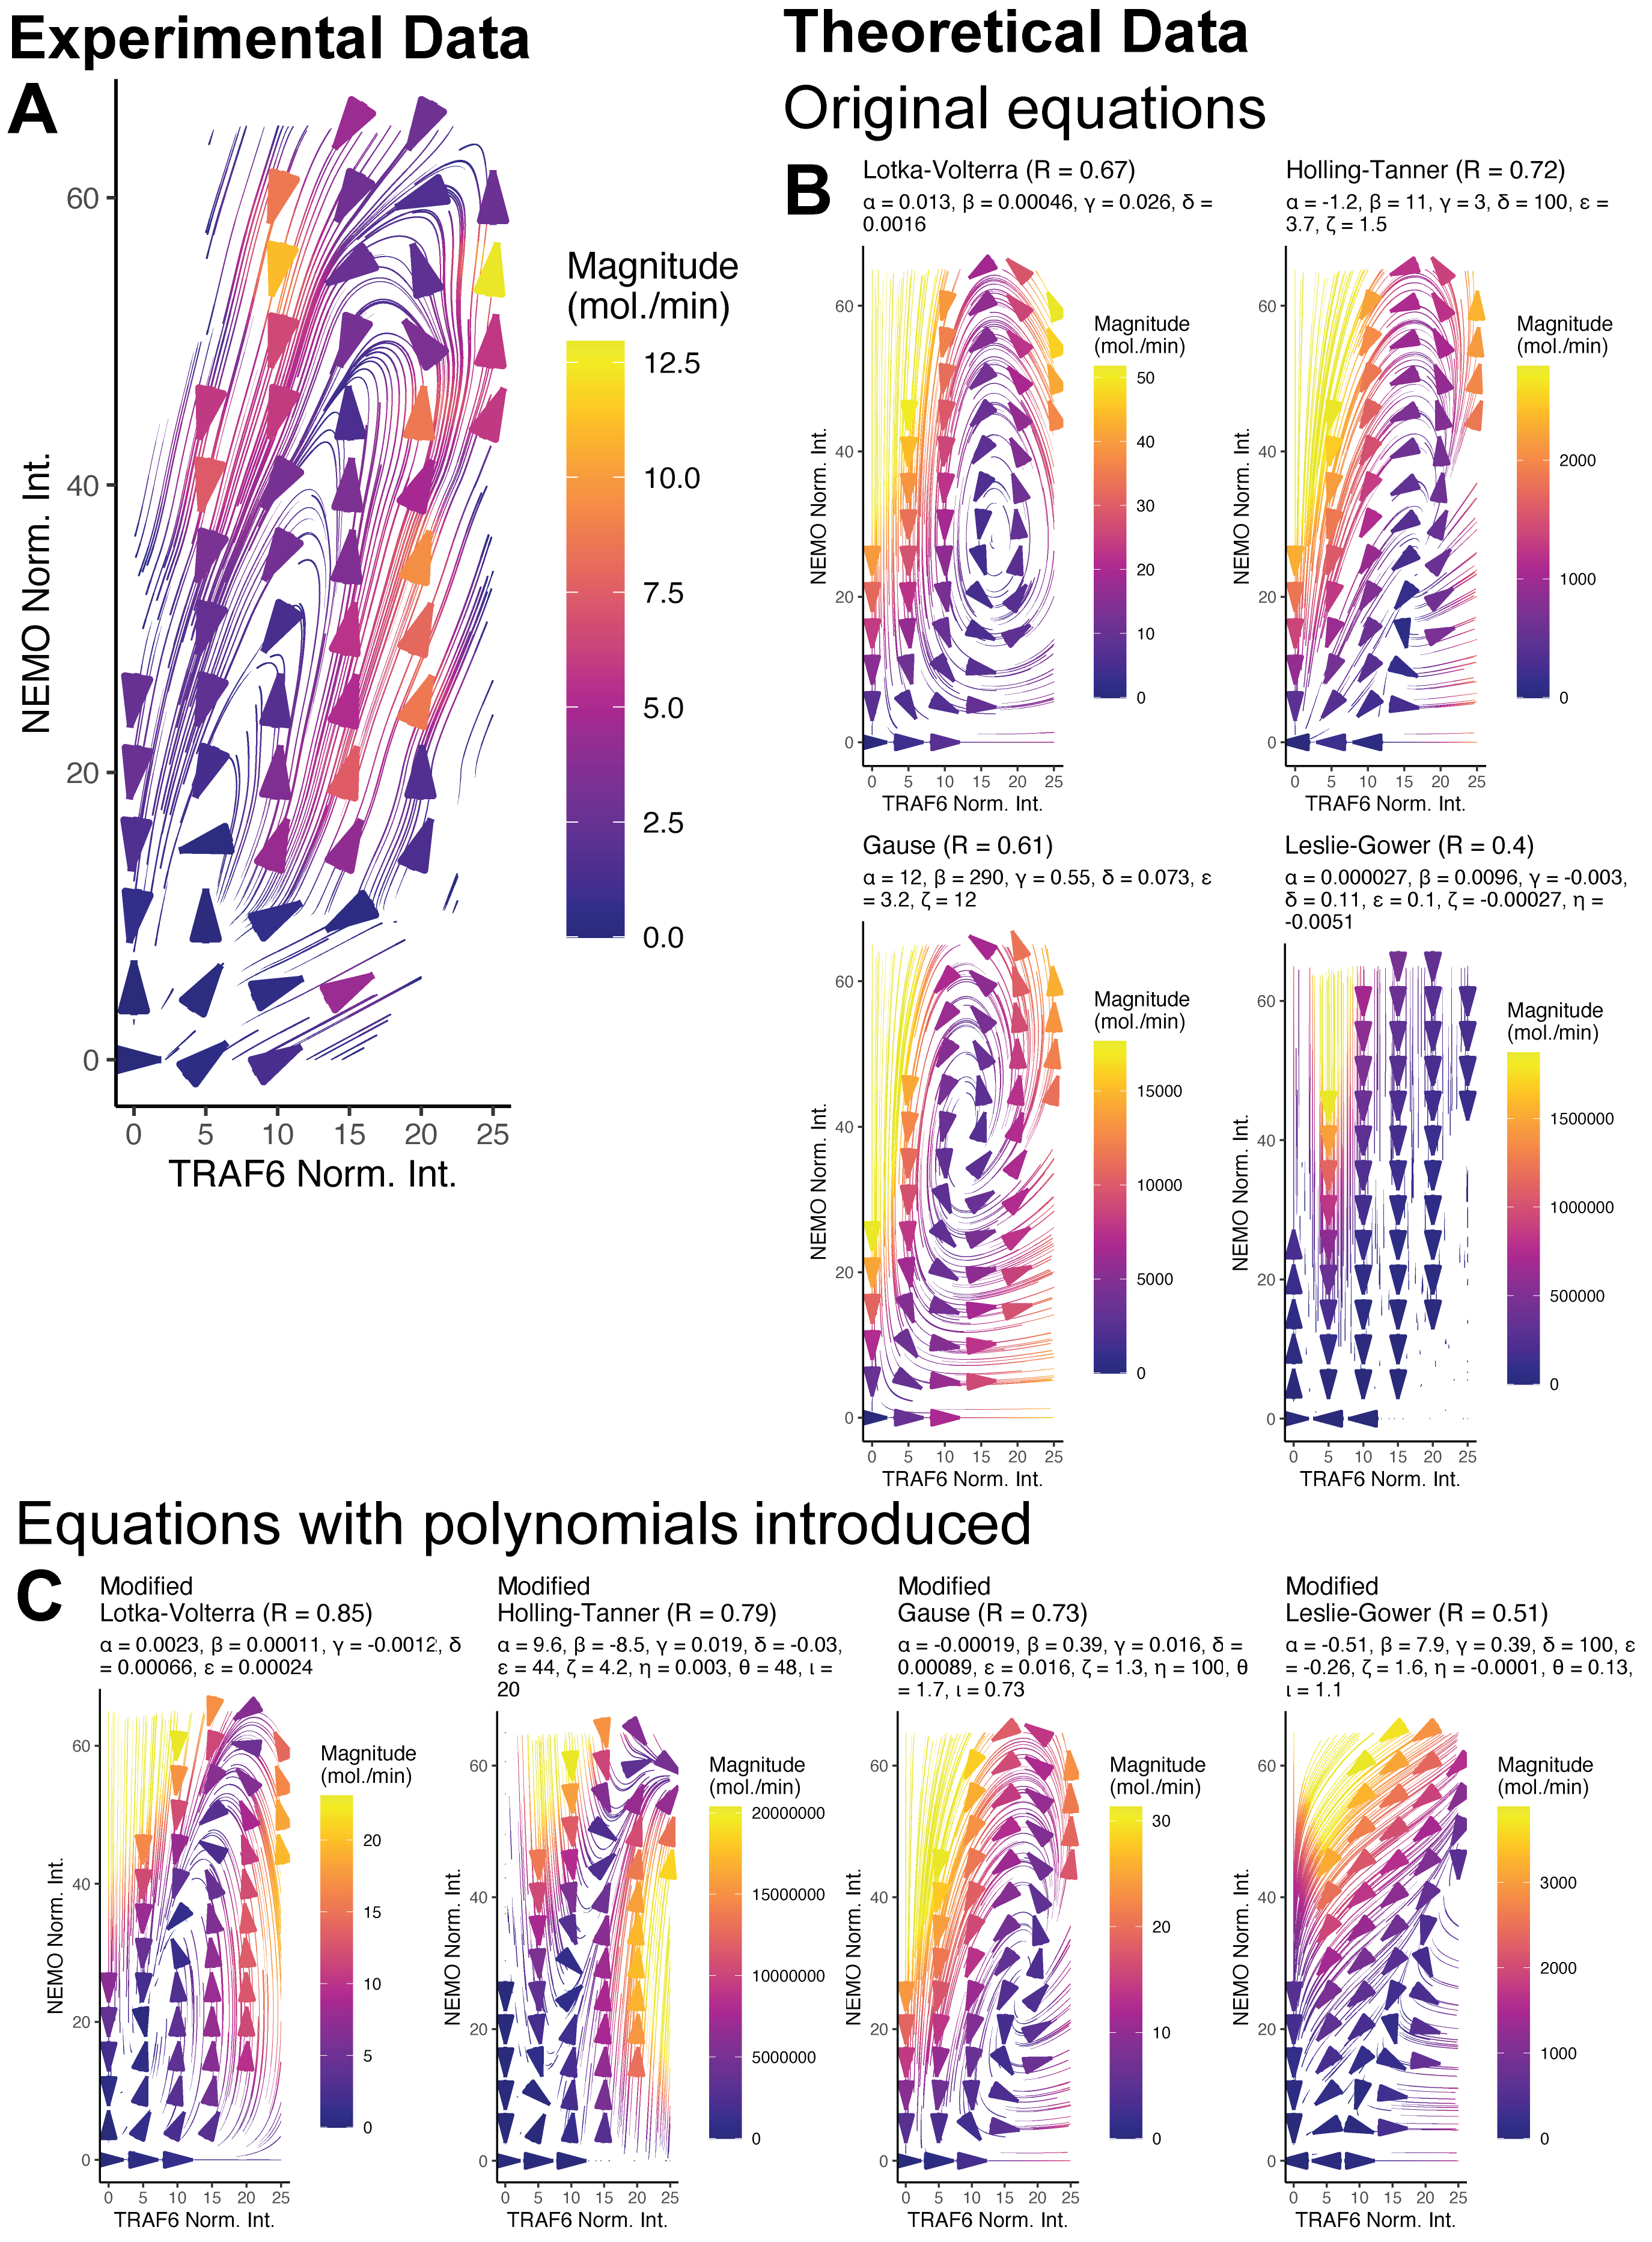
\includegraphics[width=\textwidth, height=\textheight, keepaspectratio]{mod/figS6.png}}

\captionsetup{parbox=none}
\captionof{figure}[The chaotic assembly and catastrophic disassembly dynamics of the IL-1 pathway]{\textbf{The chaotic assembly and catastrophic disassembly dynamics of the IL-1 pathway.}
\\
\\
(A) This figure presents the spiral phase portrait of NEMO-TRAF6 growth interactions, featuring elliptical orbits and diagonal symmetry. One side of the diagonal illustrates protein growth (positive), while the opposite side depicts protein disassembly (negative growth). The orbital characteristics of this phase portrait resemble the dynamics found in predator-prey interaction phase portraits.
\\
\\
(B) To model TRAF6-NEMO interactions, I employed differential equations that capture dynamic changes in these interactions. I used the Lotka-Volterra, Holling-Tanner, Gause, and Leslie-Gower predator-prey equations, and made a table of all possible parameter combinations ranging from 10\textsuperscript{-4} to 10\textsuperscript{2}. From this table, 3000 random samples were taken, and the optimal parameters were selected based on Pearson correlation coefficients and Euclidean distance. Holling-Tanner exhibited the best correlation (R = 0.72), followed by Lotka-Volterra (R = 0.67), Gause (R = 0.61), and Leslie-Gowler (R = 0.40). The parameters are denoted in Greek letters and the fitness parameters follow the equal sign. The Lotka-Volterra and Gause equations share similar visual orbits, and to a certain extent, the Holling-Tanner as well.
\\
\\
(C) To better match the experimental data, a polynomial was introduced to modify the shape of the phase portrait from the typical “D” shape seen in predator-prey models to an elliptical “0” shape. The modified Lotka-Volterra equation provided the highest correlation (R = 0.85) and best visual similarity to the experimental data. While the modified Holling-Tanner also improved its correlation (R = 0.79), it was visually less similar to the experimental data and the original equation. The modified Gause and Leslie-Gowler equations also showed improved correlations (R = 0.73 and R = 0.51, respectively), but neither surpassed the modified Lotka-Volterra in performance.
\\
\\
(A: Imaging data courtesy of Elke Ziska. Analysis, plots by the thesis author.)}
\label{p2:S6}
\end{centering}

The next step in my variable exploration involved understanding the effects of varying individual parameters on the resulting phase portraits. By manipulating one parameter at a time (Fig. \ref{p2:S7a}) or two simultaneously (Fig. \ref{p2:S7c}), valuable insights can be gained into the sensitivity and robustness of the system to changes in these variables.

Upon inspection of the modified phase portraits, I see that altering any single parameter influences the behavior of the system, yet the parameters $\delta$ and $\epsilon$ display a more impactful effect on the overall dynamics. Even minor changes in these variables result in dramatic transformations in the phase portraits, suggesting that these parameters are particularly influential in shaping the behavior of the system.


\begin{centering}
\centering{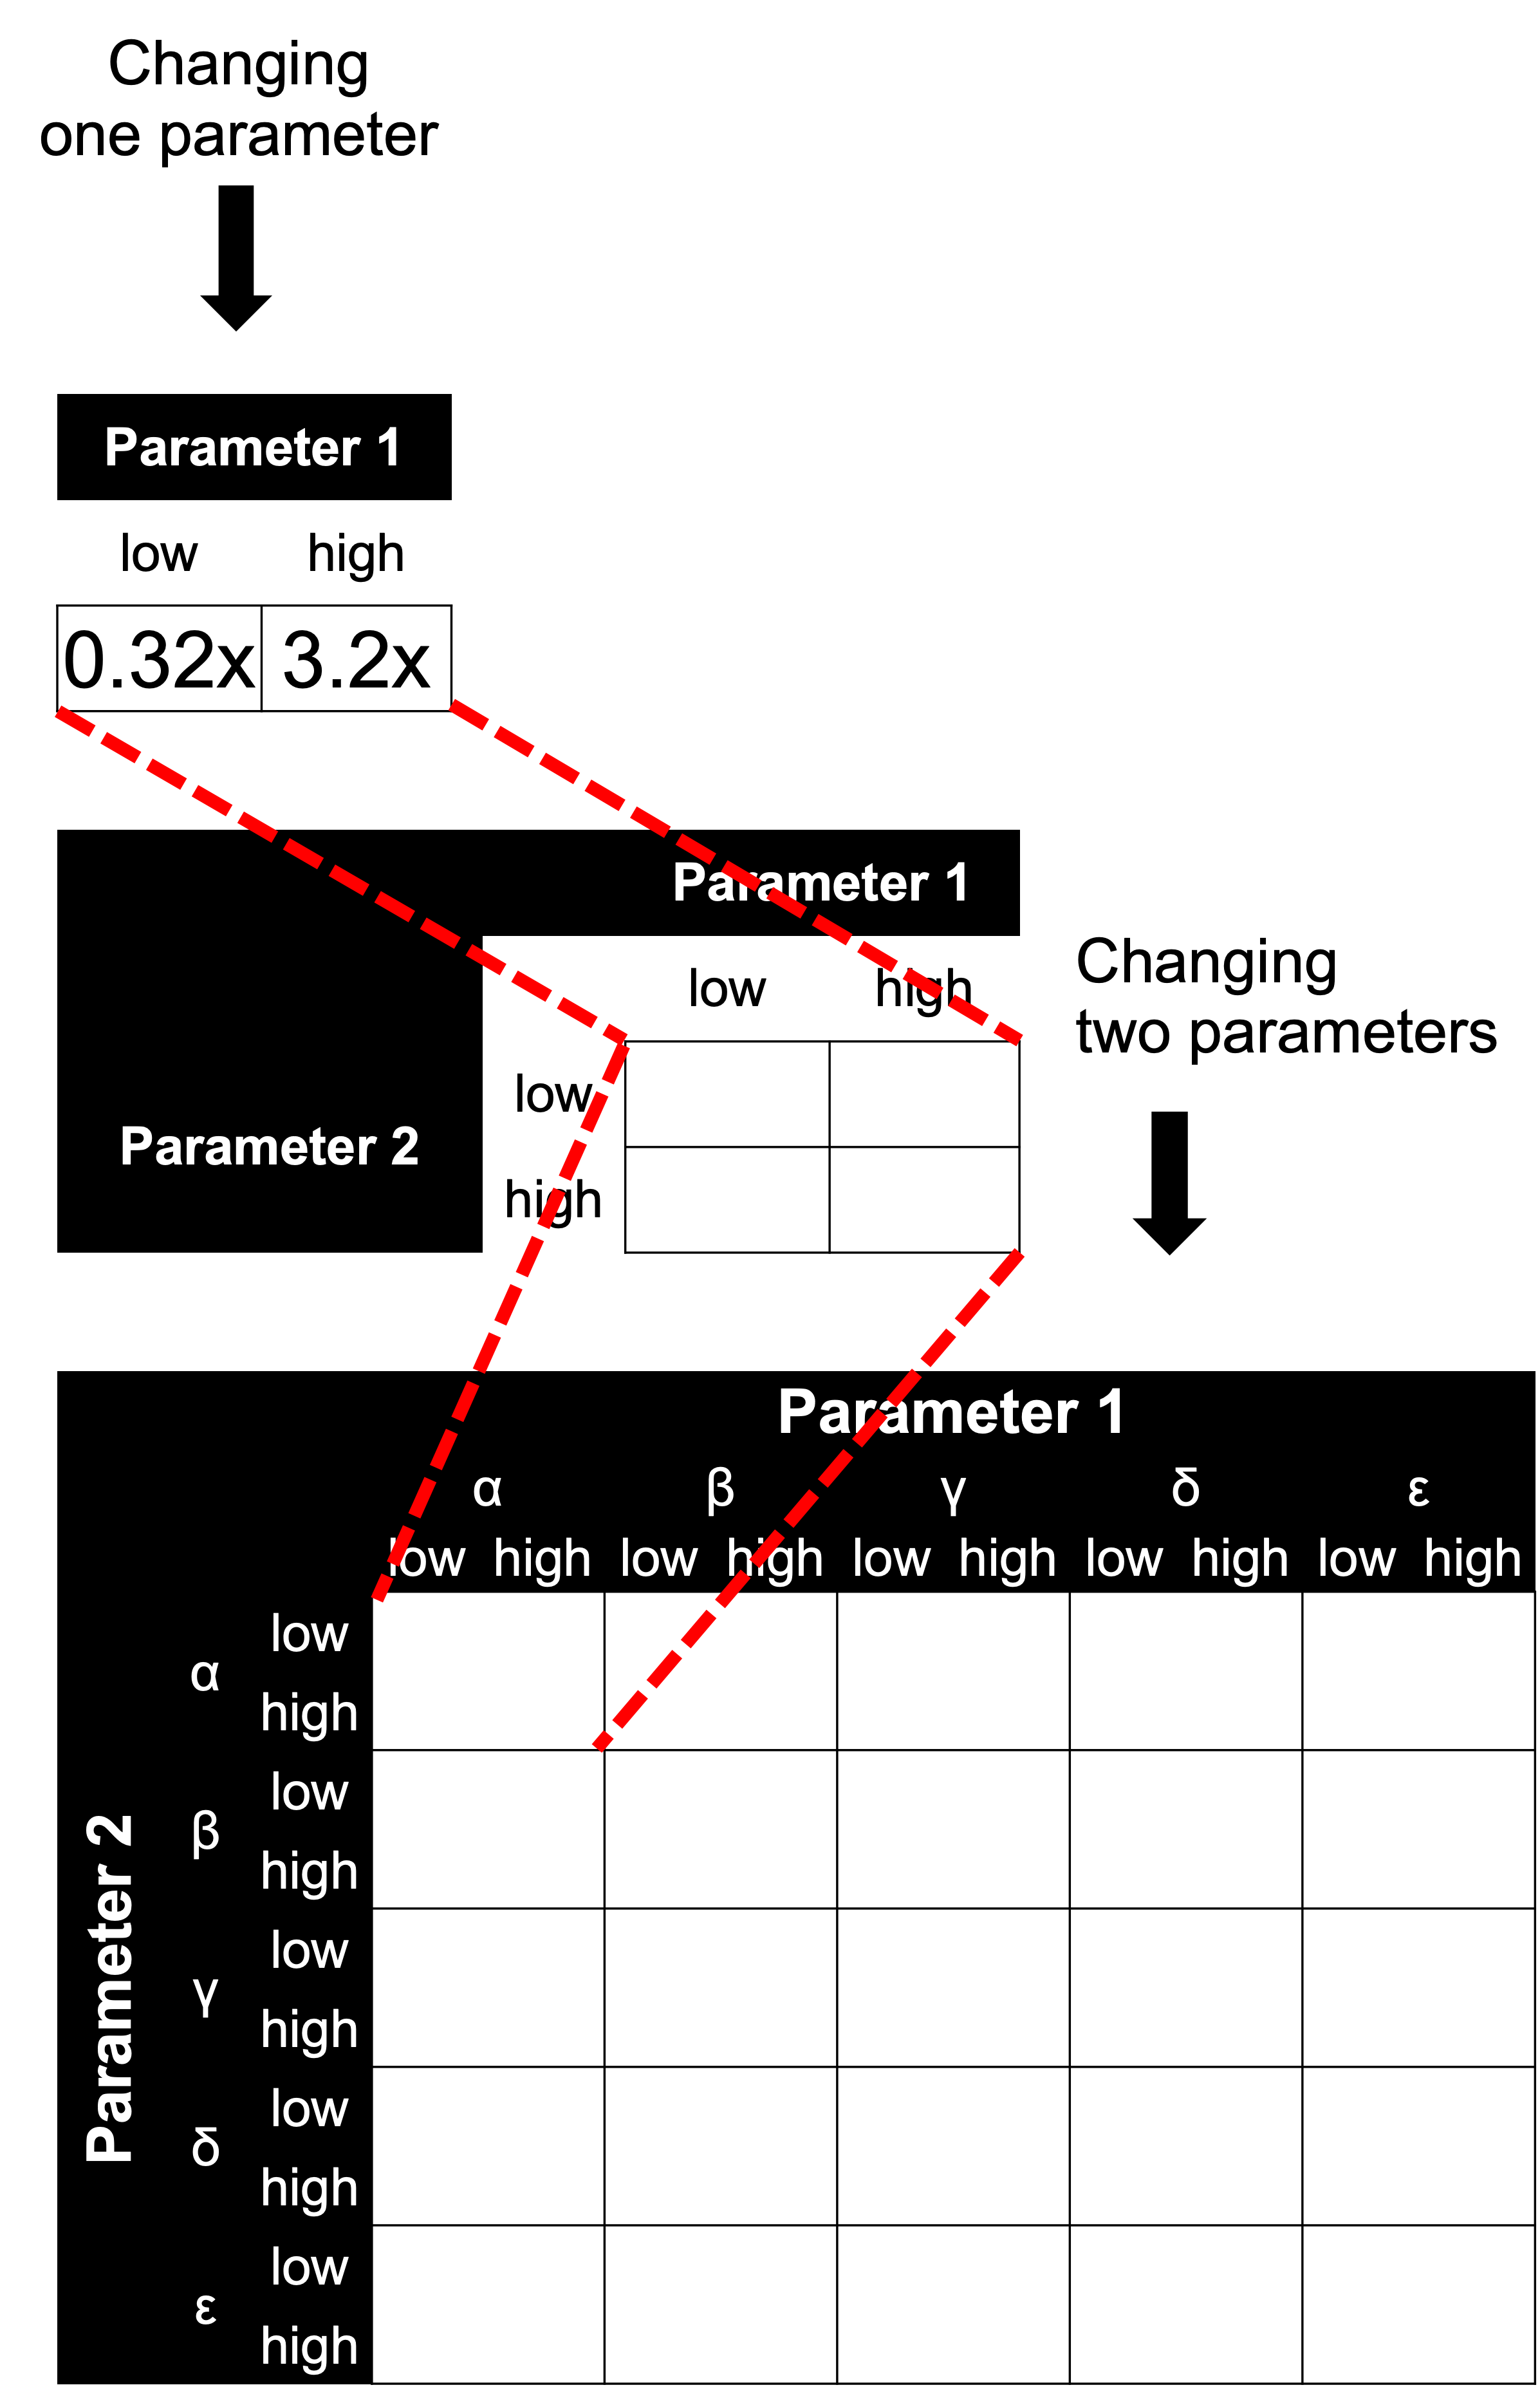
\includegraphics[width=\textwidth, height=\textheight, keepaspectratio]{mod/figS7a.png}}
\captionsetup{parbox=none}
\captionof{figure}[Schematic on how variables and parameters affect dynamics]{\textbf{Schematic on how variables and parameters affect dynamics.} I further characterized the modified Lotka-Volterra equations by multiplying the parameters by a constant and observing their phase portraits. This schematic illustrates the process. For the “Changing one parameter,” each parameter was multiplied by a decimal or a whole number to visualize the effects of lower or higher parameter values. For “Changing two parameters,” I altered two variables simultaneously, using 0.32\times (lower boundary) and 3.2\times (higher boundary), to compare variable against variable, as variable relationships in differential equations may not be evident when analyzed in isolation.}
\label{p2:S7a}
\end{centering}


\begin{centering}
\centering{\includegraphics[width=\textwidth, height=\textheight, keepaspectratio]{mod/figS7b.png}}
\captionsetup{parbox=none}
\captionof{figure}[The effects of modifying one parameter of the modified Lotka-Volterra equations]{\textbf{The effects of modifying one parameter of the modified Lotka-Volterra equations.} Each parameter was multiplied by a decimal or a whole number to visualize the effects of lower or higher parameter values. The parameters are in rows and the changes to the parameter, $y = 10^{\frac{x}{4}}$ for $x = -4 \text{ to } 1$ in columns.}
\label{p2:S7b}
\end{centering}



\begin{centering}
\centering{\includegraphics[width=\textwidth, height=\textheight, keepaspectratio]{mod/figS7c.png}}

\captionsetup{parbox=none}
\captionof{figure}[The effects of modifying two parameters of the modified Lotka-Volterra equations]{\textbf{The effects of modifying two parameters of the modified Lotka-Volterra equations.} I altered two variables simultaneously, using 0.32\times (lower boundary) and 3.2\times (higher boundary), to compare variable against variable, as variable relationships in differential equations may not be evident when analyzed in isolation. This panel demonstrates the effects of changing two variables simultaneously, using lower (0.32\times) and higher (3.2\times) values than the parameters used in Fig. \ref{p2:7}.}
\label{p2:S7c}
\end{centering}

This exercise not only enriches the understanding of the individual and combined effects of these parameters on the system, but it also illustrates how mathematical modeling can provide a powerful tool for examining complex biological phenomena. By enabling me to systematically manipulate the components of my model, I can make predictions, test hypotheses, and potentially uncover new insights into the fundamental mechanisms governing intricate biological systems like the IL-1 pathway.

\chapter{IL-1 pathway proteins show history-dependent assembly}
\chaptermark{History-dependent assembly}
\label{chapter:chaos}
\epigraph{Me detuve, como es natural, en la frase: “Dejo a los varios porvenires (no a todos) mi jardín de senderos que se bifurcan”. Casi en el acto comprendí; El jardín de senderos que se bifurcan era la novela caótica; la frase “varios porvenires (no a todos)” me sugirió la imagen de la bifurcación en el tiempo, no en el espacio. La relectura general de la obra confirmó esa teoría. En todas las ficciones, cada vez que un hombre se enfrenta con diversas alternativas, opta por una y elimina las otras; en la del casi inextricable Ts'ui Pên, opta -simultáneamente- por todas. Crea, así, diversos porvenires, diversos tiempos, que también proliferan y se bifurcan. De ahí las contradicciones de la novela.\par
\vspace{\baselineskip}
\emph{Naturally, my attention was caught by the sentence, “I leave to various future times, but not to all, my garden of forking paths: I had no sooner read this, than I understood. The Garden of Forking Paths was the chaotic novel itself. The phrase “to various future times, but not to all” suggested the image of bifurcating in time, not in space. Rereading the whole work confirmed this theory. In all fiction, when a man is faced with alternatives he chooses one at the expense of the others. In the almost unfathomable Ts'ui Pen, he chooses - simultaneously - all of them. He thus creates various futures, various times which start others that will in their turn branch out and bifurcate in other times. This is the cause of the contradictions in the novel.}}{Jorge Luis Borges\\The Garden of Forking Paths, 1941}

\section{Recapitulation}
I have observed the assembly and disassembly of the IL-1 pathway. Within the pathway, I found two signalosomes: the Myddosome signalosome and the NF-κB signalosome. The Myddosome signalosome assembles first, and it consists of MyD88, IRAK4, IRAK1, TAB2 and TRAF6. Next, the NF-κB signalosome assembles, with HOIL1 first, then NEMO, RelA and lastly, A20. The interaction between these two signalosomes can be described as a predator-prey interaction with the Myddosome module as the prey and the NF-κB signalosome as the predator (Fig. \ref{p2:7}). I formulated a set of equations derived from the Lotka-Volterra equations, but with an additional parameter for logistic-growth of the predator. My set of equations accurately describe the system with a very high Pearson correlation coefficient (R = 0.85).

\section{The paths that fork: Assembly trajectories show bifurcation}
\sectionmark{Bifurcation}
Bifurcation, in dynamical systems, implies the splitting of a system into two distinct trajectories. This phenomenon arises in bistable systems, which possess two equilibrium points. In biochemical terms, we can envision a switch with two potential states. This bifurcation mechanism plays a key role in several biological pathways, such as glycolysis, MAPK/ERK, and hemoglobin, introducing regulatory complexity into the system (Jacobsen \& Trane, 2010; Shiraishi et al., 2010).

My hypothesis is that in IL-1 signaling, stoichiometries may bifurcate into two distinct assembly categories, potentially due to the existence of two or more stable stoichiometries and varied assembly mechanisms. I predict two distinct assembly trajectories: one beginning with the growth of MyD88, and the other led by the downstream protein. To investigate this hypothesis, I analyzed our microscope data.

In examining multiple cell lines, I observed two types of assembly dynamics: one where MyD88 reaches mid-intensity first, and another where the downstream protein takes the lead, as observed in the MyD88-TRAF6 cell line (Fig. \ref{p3:1}A). This observation substantiates my hypothesis but does not provide information regarding the frequency of these dynamics. It raises questions about whether proteins consistently maintain the same stoichiometric ratios from initiation to completion, or not. To address this, I performed a 2D density plot comparing the starting and ending stoichiometries, using the percentage of MyD88 in the complex as the stoichiometric ratio.

Generally, most puncta maintain the same stoichiometry from start to end (depicted by the diagonal line), with exceptions being IRAK1, TRAF6, NEMO, TAB2, and RelA, where some puncta deviate from the diagonal line (Fig. \ref{p3:1}C). This ratio shift indicates potential candidates for bifurcation. Yet, it does not provide insight into the underlying mechanism of this shift. To explore whether proteins transition between assembly trajectories and understand how different proteins enrich the assemblies, I created phase portraits of the stoichiometric ratios (percentage of MyD88 in the puncta) over time, with frequency colorized and arrow angle indicating the growth direction.

Analysis of the stoichiometry phase portraits reveals that usually, MyD88 growth precedes the joining of the downstream protein. Notably, IRAK1, TRAF6, NEMO, TAB2, and RelA data bifurcate around the 40-second mark of puncta time. In the case of the MyD88-IRAK1 cell line, assemblies richer in IRAK1 tend to abort earlier, while those richer in MyD88 appear more stable, a pattern that is consistent with TRAF6 and TAB2. Interestingly, for NEMO and RelA, we observe a bistable system, where both MyD88-rich and NEMO/RelA-rich assemblies persist for similar durations. The best predictor of the final stoichiometric ratio is the initial stoichiometric ratio (Fig. \ref{p3:1}D), suggesting that the assembly of the IL-1 pathway is deterministic in nature.


\begin{centering}
\centering{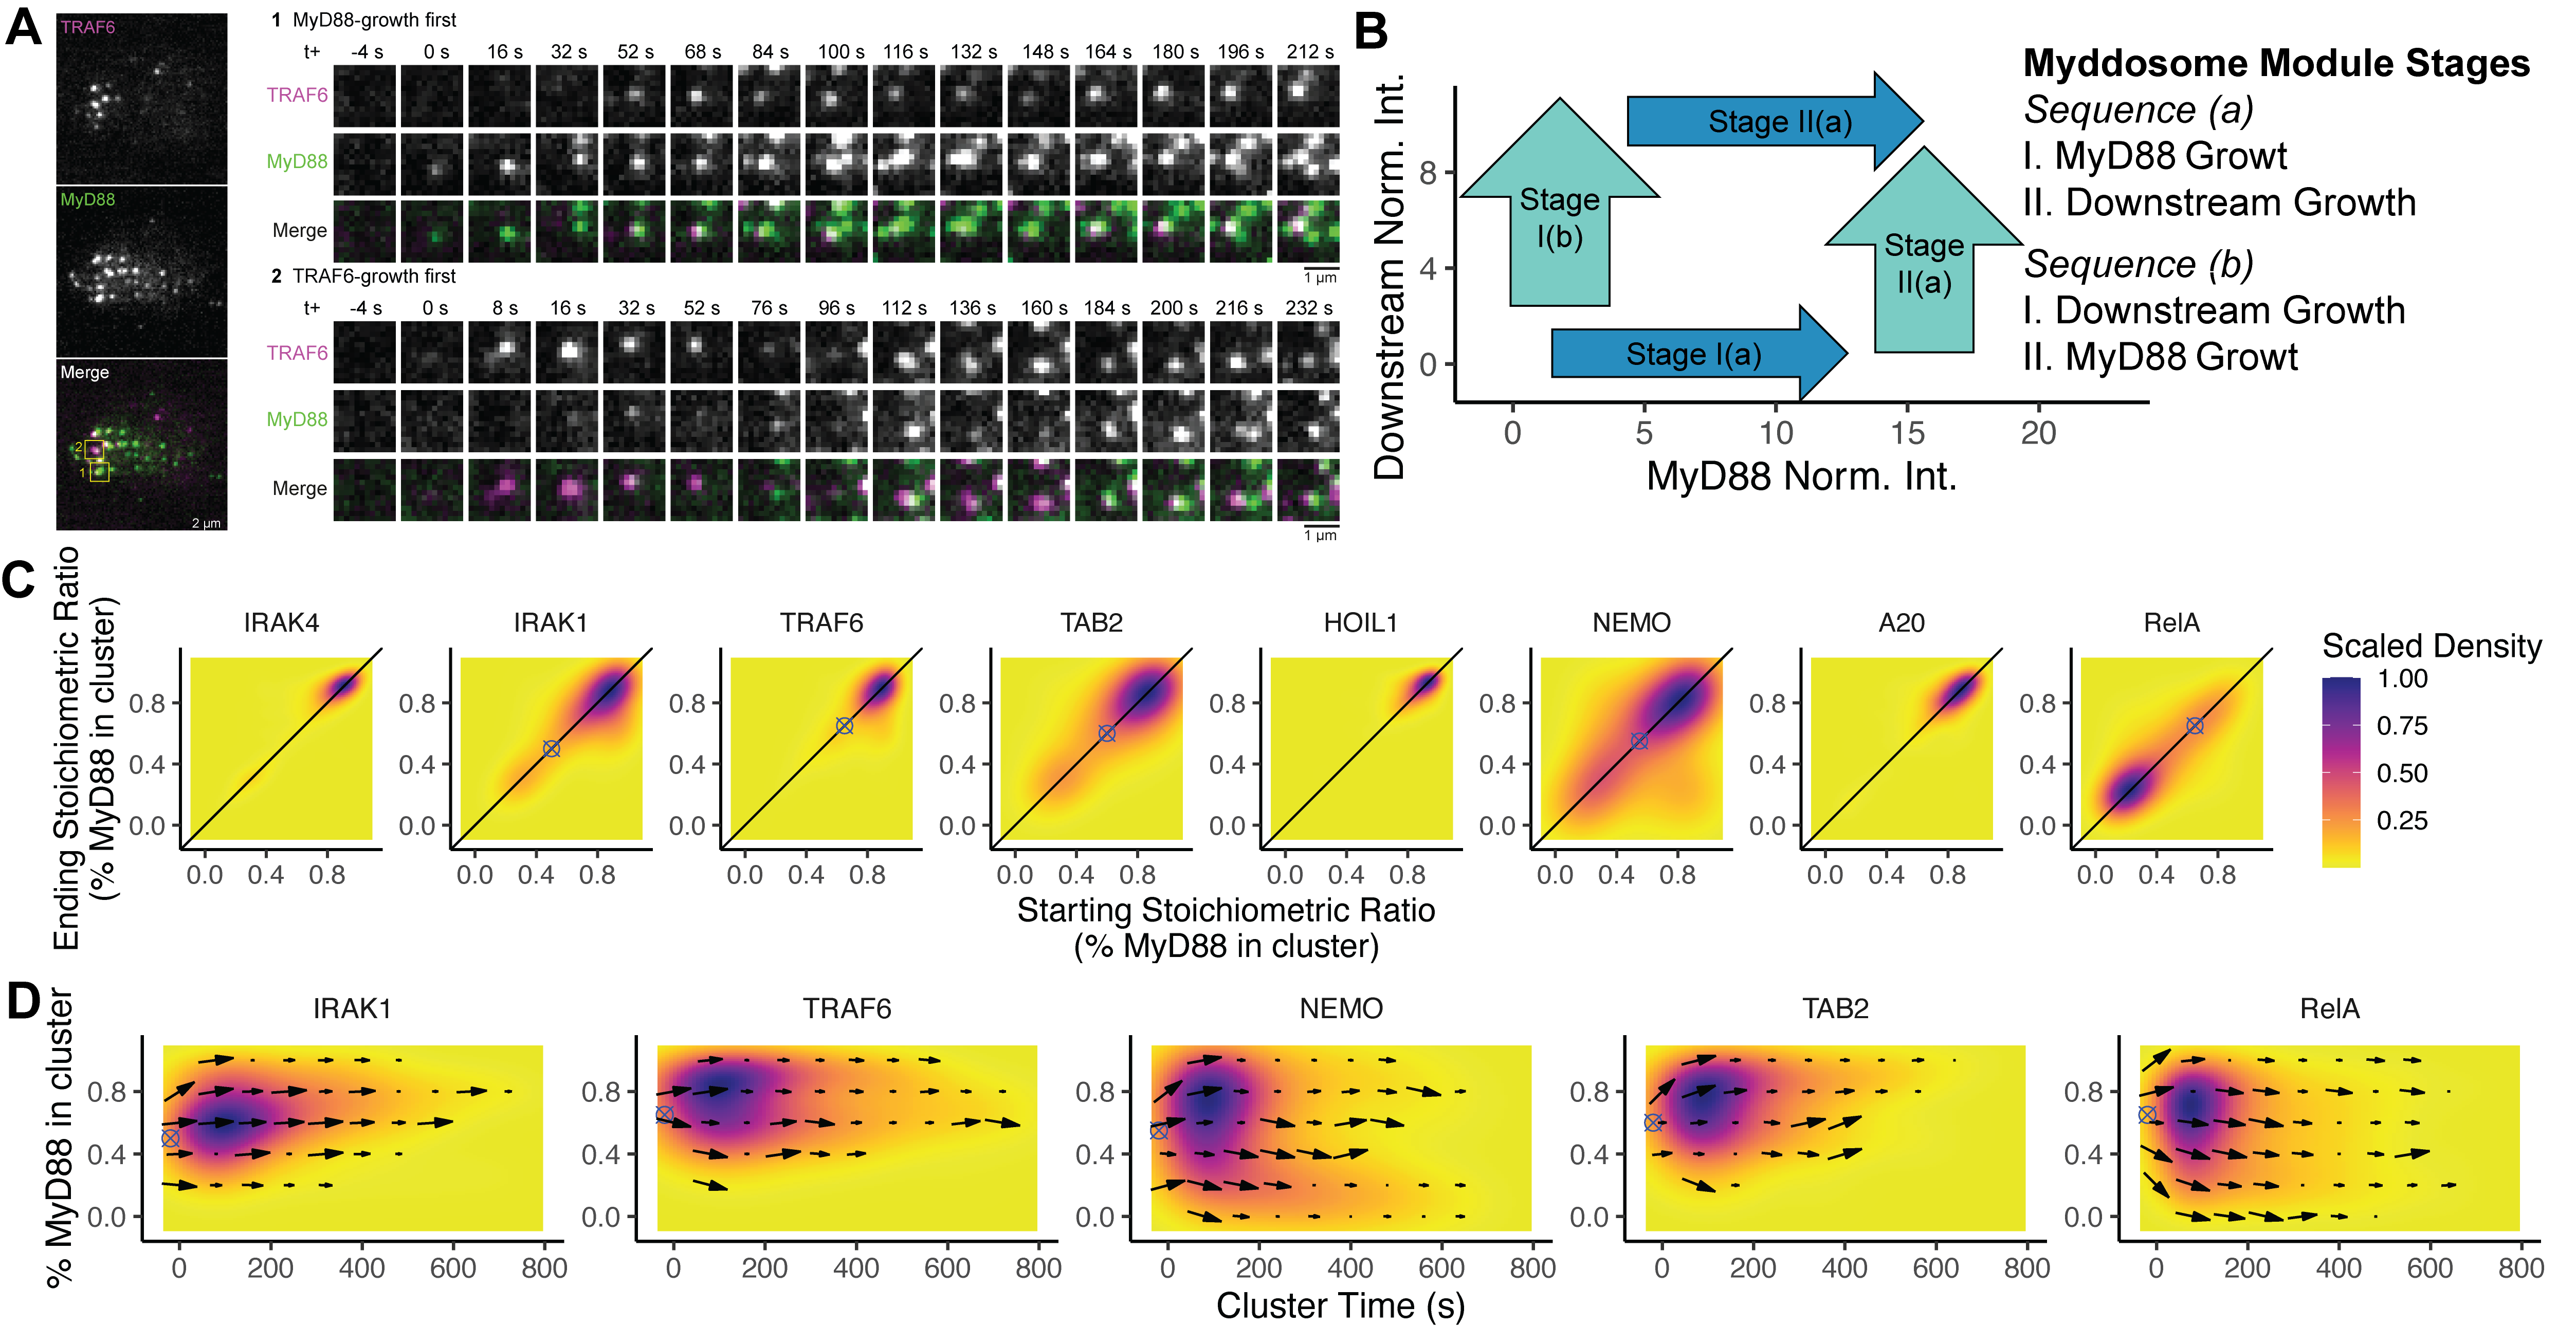
\includegraphics[width=\textwidth, height=\textheight, keepaspectratio]{chaos/fig1.png}}
\captionof{figure}[Stoichiometric analysis of MyD88 and other IL-1 pathway proteins show bifurcated trajectories and chaotic dynamics]{\textbf{Stoichiometric analysis of MyD88 and other IL-1 pathway proteins show bifurcated trajectories and chaotic dynamics.} 
\\
\\
(A) During visual inspection of microscope images, I observed that MyD88 often appeared and grew before recruiting downstream proteins. I termed this “MyD88-growth first.” However, in some cases, the downstream protein was present without colocalized MyD88, which I called “downstream protein-growth first.” Here, I show an example of each type of puncta, (1) MyD88 and (2) downstream protein growth first, for the MyD88-TRAF6 cell line.
\\
\\
(B) This schematic illustrates the assembly scenarios of (a) MyD88 growth first and (b) downstream protein growth first.
\\
\\
(C-D) I calculated the stoichiometric ratio for each puncta by dividing MyD88 size by the sum of MyD88 and downstream protein sizes, which indicates the percentage of MyD88 in the puncta. High percentages are called MyD88-rich, and low percentages are downstream protein-rich.
\\
\\
(C) This 2D density plot compares the starting and ending stoichiometric ratios of puncta, with color indicating the frequency of events. Points on the diagonal line indicate unchanged beginning and ending stoichiometries. Except for RelA (due to artifact tracking), most puncta started and ended MyD88-rich (top-right corner). IRAK1, TRAF6, NEMO, TAB2 and RelA cell lines show puncta changing stoichiometric ratios during assembly, with different starting and ending stoichiometries.
\\
\\
(D) For these cell lines, I plotted stoichiometry over time as a 2D density plot with overlaid phase portraits. Arrows pointing up indicate MyD88 addition, while arrows pointing down indicate downstream protein addition, with magnitude showing the amount of protein added. I noticed bifurcated (forked) trajectories around 60\% MyD88 in some cell lines and filtered data to include only puncta with an initial stoichiometric ratio within $\pm$15\% of the blue crossed circle, enhancing bifurcation visibility. Bifurcation was especially evident in NEMO and RelA. While NEMO and RelA are observed at the plasma membrane, the puncta displayed here initially contained MyD88 and subsequently became enriched with downstream proteins. Once a punctum adopted a specific trajectory, it remained unchanged.
\\
\\
(C-D) The starting stoichiometry was a good indicator of the ending stoichiometry, with a sensitive dependence on initial conditions, but it could not perfectly predict the ending stoichiometry. These findings suggest that IL-1 assembly is triggered by chaotic dynamics.
\\
\\
(A: Panel courtesy of Fakun Cao. C-D: Imaging data courtesy of Fakun Cao, Niranjan Srikanth, Elba del Val Oriza and Claudia Abad-Baucells. Analysis, plots by the thesis author.)}
\label{p3:1}
\end{centering}

Indeed, the Lotka-Volterra equations predict deterministic trajectories. Deterministic processes are those whose trajectory can be predicted, which in my case would be with a solved modified Lotka-Volterra equation (see the end of Results~\ref{chapter:p2}). Stochasticity, on the other hand, would be the complete opposite, that is, the process cannot be predicted. Biochemically, these two concepts are not at odds with each other. A deterministic process can have variance emerge stochastically. Also, a stochastic looking process can be deterministic. This would be chaotic dynamics. Here, we observed history-dependent trajectories, consistent with chaotic dynamics. However, this would require further mathematical work beyond the scope of this thesis.

Whether both are capable of signaling or not is unknown. Assuming both trajectories described above are capable of signaling, one physiological reason two assembly mechanisms might exist in the IL-1 pathway is to have one quick signal that degrades quickly and another that takes longer to assemble but the signal persists for longer. The alternate hypothesis would be that one of these two trajectories does not signal. That is, if the complex assembles using the wrong steps, then this will not signal. It would need to have the correct stoichiometric ratio and timing to be able to transduce a signal. This process would be akin to kinetic proofreading in that high specificity can be achieved by introducing a temporal delay, termed proofreading. The system only goes forward if the kinetics are right. Independent but congruent with the two hypotheses, a physiological reason for bifurcation would be for introducing self-regulation, or simply a byproduct of the regulatory dynamics (Del Vecchio et al., 2018).

\section{Assemblies have a critical stoichiometry}
\sectionmark{Critical stoichiometries}
If the trajectories fork, then there must be a bifurcation point where the trajectories split from. Because my previous phase portrait compared the stoichiometric ratio over time, then the bifurcation point would be called a critical stoichiometric ratio. This critical stoichiometric ratio would have a few features. At this point, the correlation between the initial and final stoichiometry should be low, and the variability of the final stoichiometry should be high. I expected that the critical stoichiometric ratio (bifurcation threshold) would have the lowest association between the initial and final stoichiometry, and the lowest final stoichiometric ratio variance (Fig. \ref{p3:S1}A).

At around 60\% MyD88 (with some flexibility across proteins), the correlation between the starting and ending stoichiometric ratios dipped (Fig. \ref{p3:S1}B). The variance also showed that at these stoichiometric ratio regimens, the variability was high (Fig. \ref{p3:S1}C). All in all, the system is most unstable at 60\% MyD88, which would also be the bifurcation point.

Using the correlation and variance two parameters, I identified a threshold (circled x) to split the data in three: I categorized the data into MyD88-rich , TRAF6-rich, and an intermediate regimen (Fig. \ref{p3:S1}E). The bifurcation of the stoichiometric ratio of the assembly became clearer (Fig. \ref{p3:S1}E). This is evidence that the initial conditions dictate the ending conditions. MyD88 growth first is dependent upon the initial stoichiometric ratio.

Based on this, and that the assembly size is small at the beginning of assembly, I hypothesize that the assembly trajectories can be shifted with just probing of one of the proteins. Further testing would be needed to validate this, perhaps with the use of optogenetics to control binding.
 

\begin{centering}
\centering{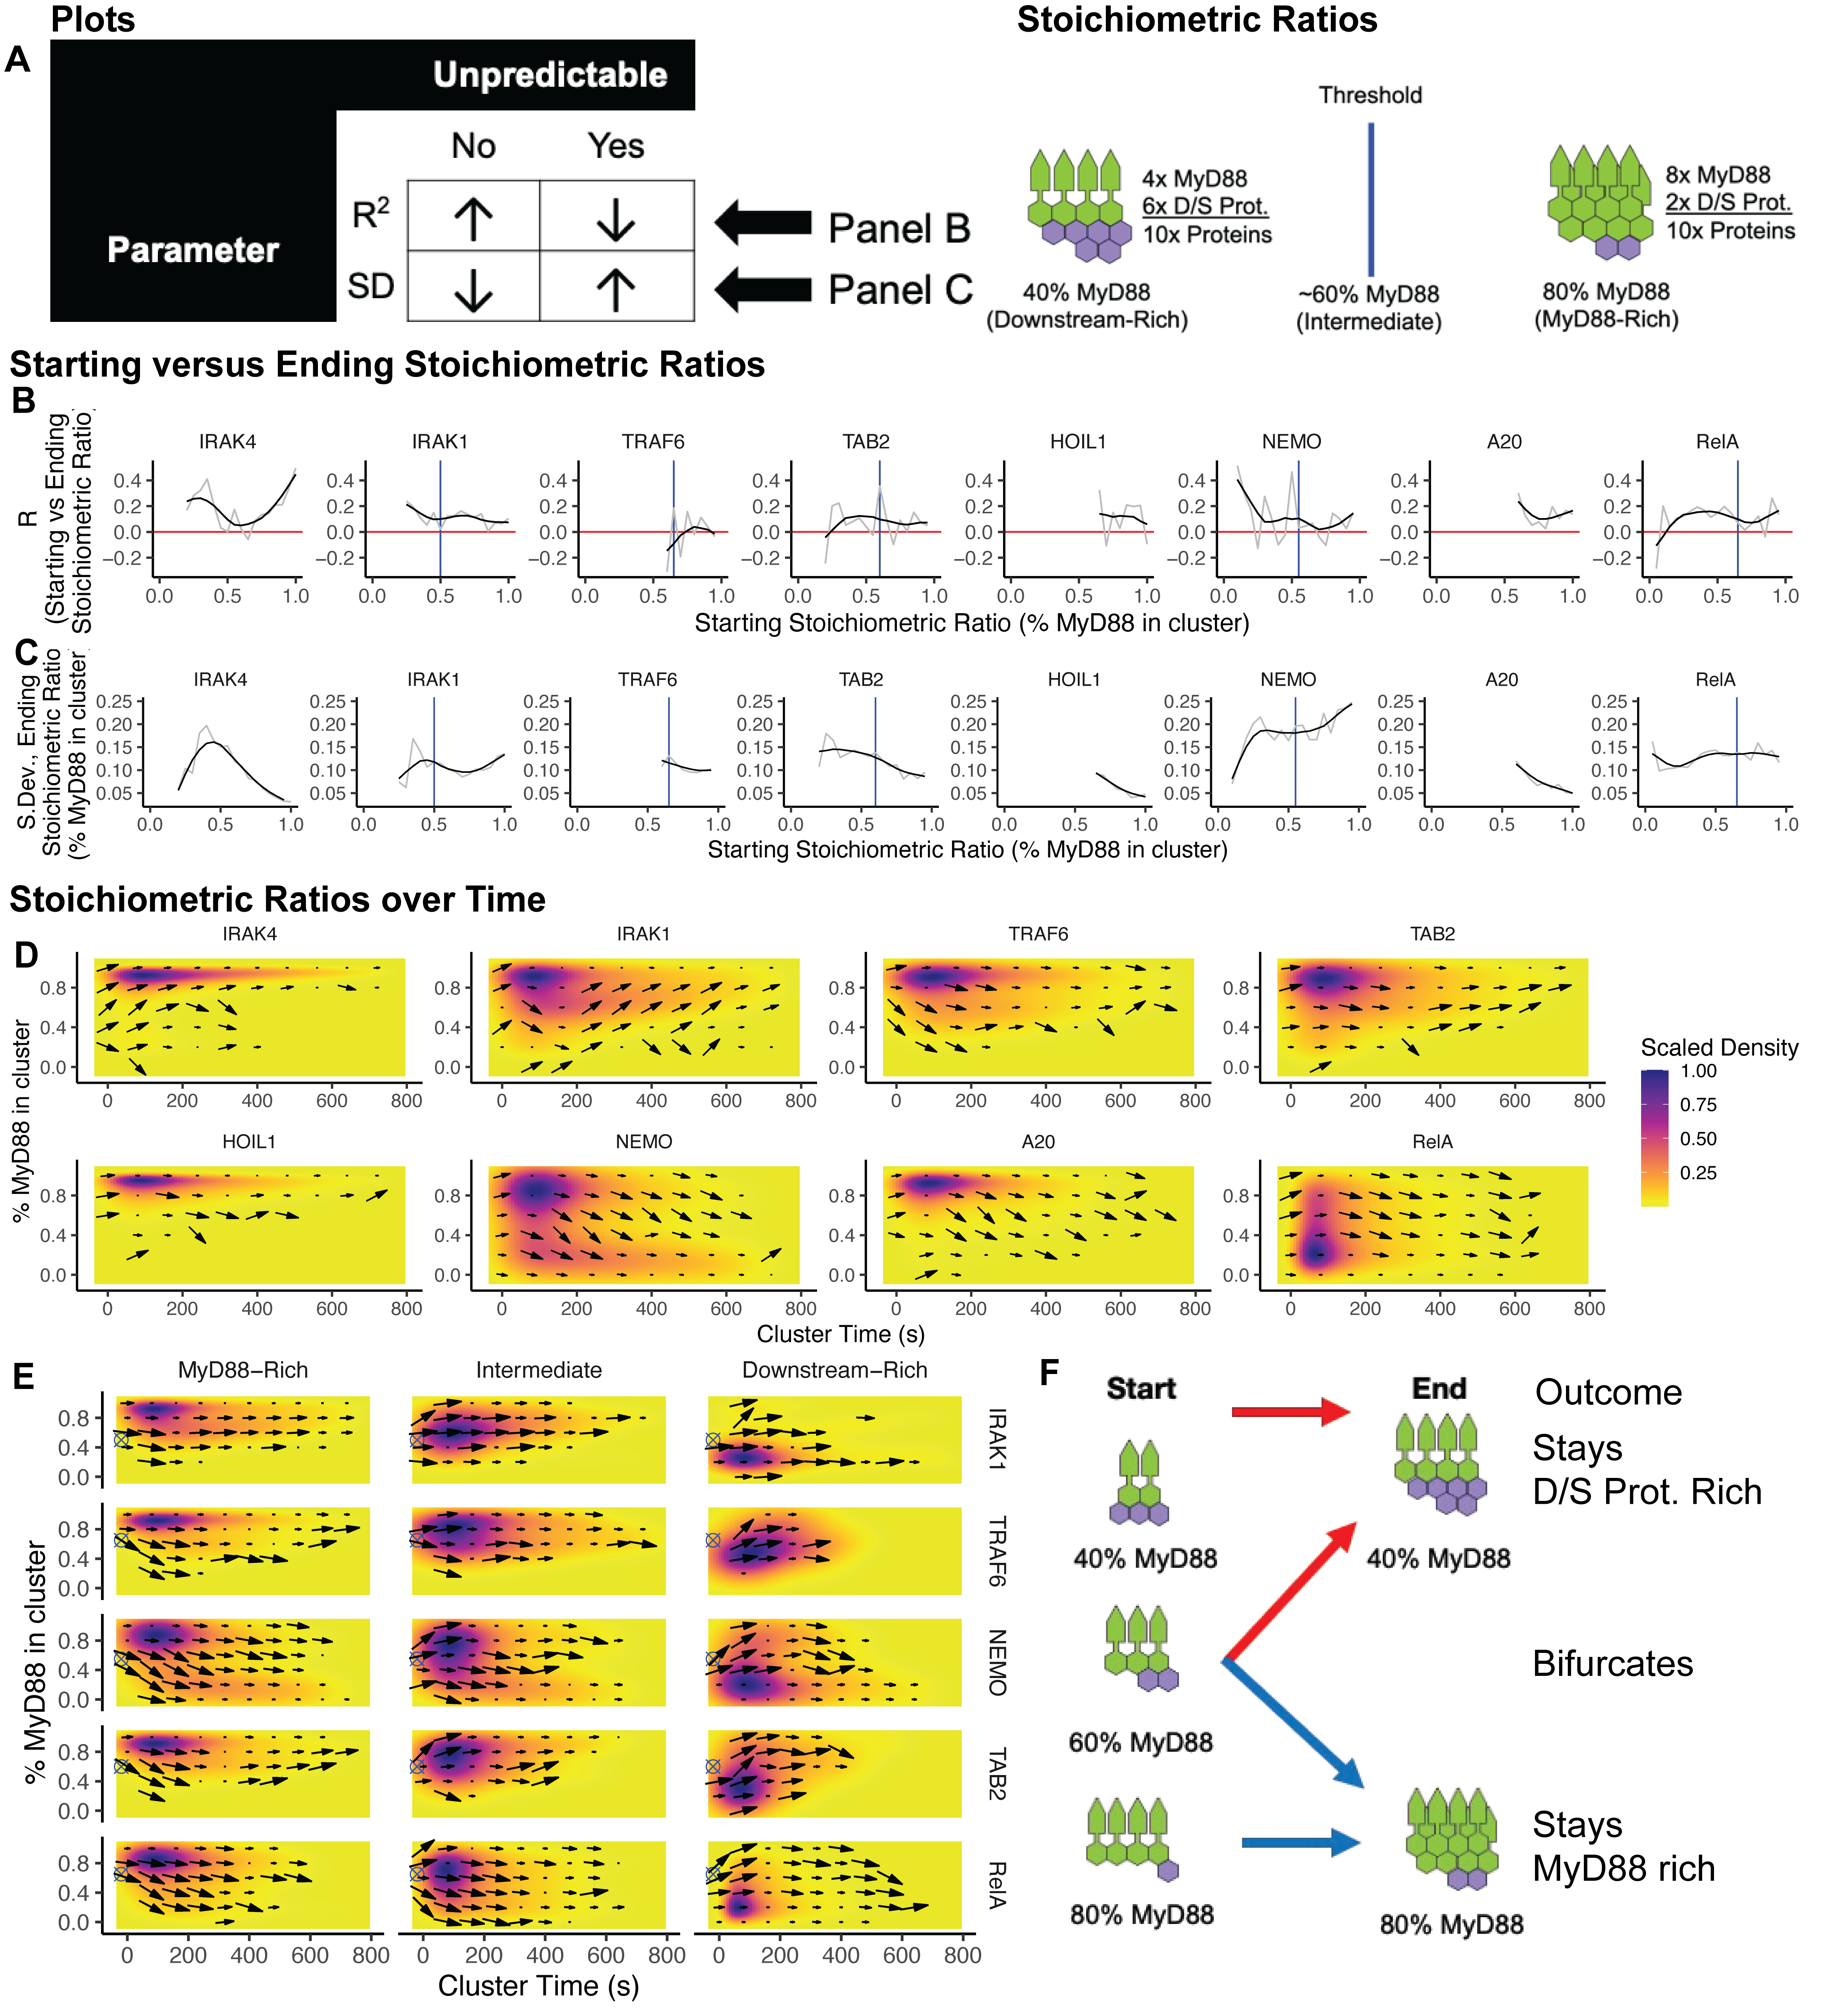
\includegraphics[width=\textwidth, height=\textheight, keepaspectratio]{chaos/figS1.png}}
\captionof{figure}[Chaotic dynamics in IL-1 assembly evident from bifurcations in the early stoichiometric ratios]{\textbf{Chaotic dynamics in IL-1 assembly evident from bifurcations in the early stoichiometric ratios.}
\\
\\
(A) The stoichiometric ratios of various cell lines over time were plotted on a 2D density plot, with a phase portrait overlay. Upward arrows represent MyD88 growth, while downward arrows indicate downstream protein growth. Arrow size corresponds to the magnitude of growth. Bifurcated trajectories were observed in several cell lines, suggesting that the initial stoichiometric ratio might determine the final ratio. However, the exact point at which assemblies are more likely to bifurcate (switch) trajectories remains unknown. Bifurcation means the data splitting from one steady state to the other. It can be triggered by chaotic behavior. Critical stoichiometry means small changes lead to big changes in assembly behavior. Because both sit at the intersection of switch-like behavior, I hypothesized that the bifurcation point and the critical stoichiometric ratio would be close to each other.
\\
\\
(B) The critical point would exhibit low correlation between the initial and final stoichiometry, and high variability in the ending stoichiometry. Correlation and standard deviation were measured to assess these properties. Unpredictable ending stoichiometries would have low correlation coefficients (R\textsuperscript{2}) and high standard deviations (SD) relative to the starting stoichiometry. Conversely, high correlation coefficients and low standard deviations would imply predictability of the ending stoichiometry based on the starting stoichiometry.
\\
\\
(C) The stoichiometric ratio is defined as the MyD88 size divided by the sum of MyD88 and downstream protein sizes. Thresholds are marked with a blue line.
\\
\\
(D) Correlations between initial and final stoichiometries were calculated, and local minima (valleys) were visually identified.
\\
\\
(E) Standard deviations in ending stoichiometries for different initial values were calculated, and local maxima (hills) were visually identified. High variability points roughly coincided with points of low correlation between initial and final stoichiometries. The most unpredictable point is marked with a blue line.
\\
\\
(F) Stoichiometry phase portraits were divided into three categories based on their initial stoichiometry: MyD88-rich, intermediate, and downstream-rich. The intermediate phase portraits are within $\pm$15\% of the threshold (blue line). MyD88-rich and downstream protein-rich portraits are above and below the line, respectively. The intermediate phase portraits exhibit the most dramatic bifurcation. The bifurcation point correlates with the initial stoichiometry, as arrows above the critical threshold point up, and those below the threshold point down. Overall, there is a critical starting stoichiometric ratio that causes the puncta to bifurcate in protein growth trajectories.
\\
\\
(A-B, D-G: Imaging data courtesy of Fakun Cao, Niranjan Srikanth, Elba del Val Oriza and Claudia Abad-Baucells. Analysis, plots by the thesis author.)}
\label{p3:S1}
\end{centering}

The heterogeneity of assembly stoichiometries and stoichiometric ratios suggest that the data is stochastic. Upon closer examination, however, I found that the data can be accurately modeled with modified Lotka-Volterra equations. One feature of Lotka-Volterra equations is that they predict a deterministic process. 

While individual assemblies showed that there are diverse stoichiometries, they nevertheless converged at stable points (Fig. \ref{p3:S1}D). For NEMO and RelA, bistability was observed: two stoichiometric ratios were stable over time (Fig. \ref{p3:1}D). The best predictor of which assembly mechanism the pathway would use was the initial stoichiometry. The sensitive dependence upon initial conditions, the deterministic nature of the assemblies, and the theoretically predictable yet experimentally unpredictable nature of the puncta lead me to conclude that the IL-1 pathway assembles through a chaotic-deterministic process. Because assemblies start small, this means that the shift in stoichiometric ratios are due to protein probing. In other words, protein probing alone is enough to shift the dynamics of the IL-1 pathway.


\chapter{IRAK4 has multiple assembly trajectories}
\chaptermark{IRAK4 trajectories}
\epigraph{The displacement of a single electron by a billionth of a centimeter at one moment might make the difference between a man being killed by an avalanche a year later, or escaping.}{Alan M. Turing\\Computing Machinery and Intelligence, 1950}

The Myddosome exhibits a variable MyD88 stoichiometry, fluctuating between 6-8\times MyD88 (Moncrieffe et al., 2020). Notably, the phase portraits of the Myddosome signalosome module suggest that there is not a single trajectory, but rather multiple trajectories towards assembly (Fig. \ref{p2:S2}A, \ref{p2:S1}B). However, this conclusion was drawn based on averaged data. To determine whether individual puncta shift their stoichiometries over time, it would be necessary to plot time traces of individual puncta.

Upon closer inspection, I noticed the MyD88-IRAK4 puncta switching between different stoichiometries (Fig. \ref{p2:S2}A). The time trace analysis revealed some variability in the timing of IRAK4 binding to MyD88. While IRAK4 preferentially binds to larger MyD88 assemblies, it could also bind to smaller MyD88 assemblies (Fig. \ref{p2:S2}B). This confirms a degree of flexibility in protein binding. A simplified interpretation of these results is presented in the kinetic diagram (Fig. \ref{p2:S2}C). One model is that monomers might insert themselves into assembled Myddosomes, or alternatively, the assembled Myddosomes themselves exhibit variable stoichiometries.

To conclusively determine which model holds true, additional data from fluorescence recovery after photobleaching (FRAP) experiments is needed. The proposed experiment would bleach MyD88 in puncta containing both MyD88 and IRAK4, within an early time frame (less than 5 minutes) post IL-1 stimulation. My hypothesis is that once IRAK4 binds stably, MyD88 doesn't exhibit recovery. I also predict that unstable MyD88 (i.e., recovering MyD88) might temporarily recruit IRAK4, but IRAK4 would disengage soon afterwards.

These insights could help understand why were multiple assembly trajectories observed in the phase portraits of Results~\ref{chapter:p2}.


\begin{centering}
\centering{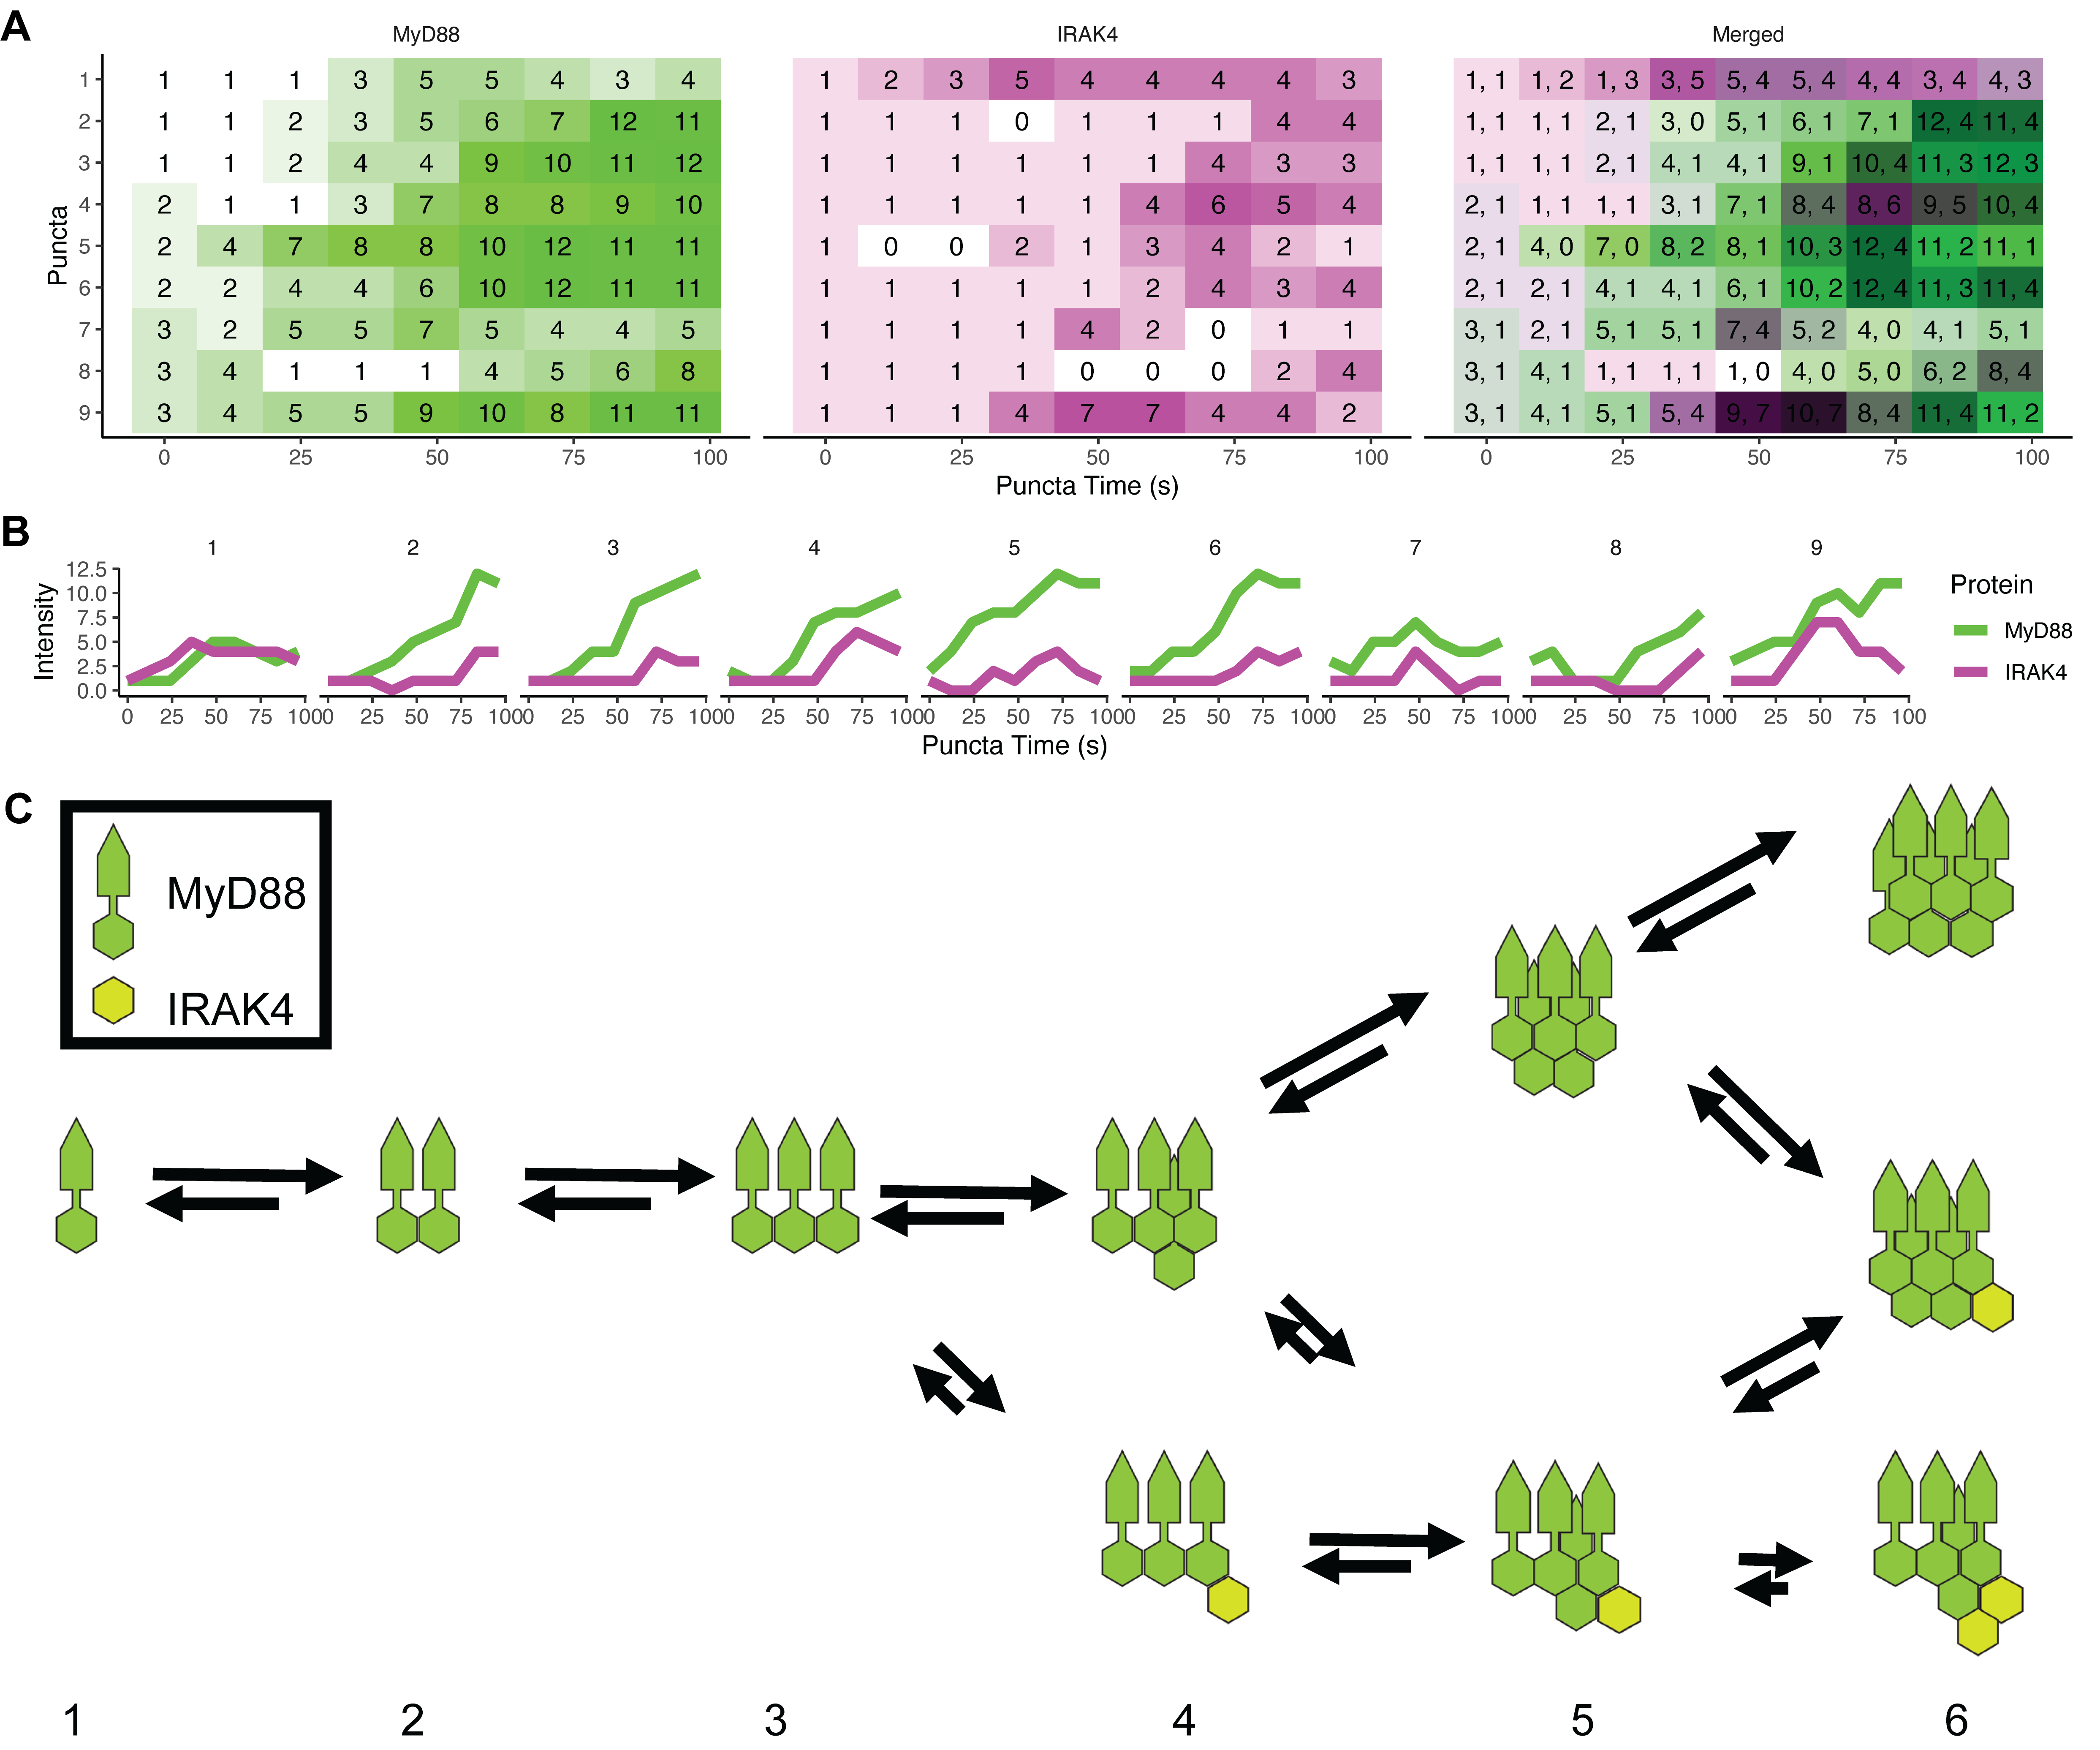
\includegraphics[width=\textwidth, height=\textheight, keepaspectratio]{chaos/fig2.png}}
\captionof{figure}[Time-traces of MyD88-IRAK4 assembly highlight the prevalence of MyD88 growth before IRAK4 growth, and also the occurrence of coassembly events]{\textbf{Time-traces of MyD88-IRAK4 assembly highlight the prevalence of MyD88 growth before IRAK4 growth, and also the occurrence of coassembly events.} (A) The heatmap displays the temporal progression of nine selected trajectories, illustrating various stoichiometries of MyD88-IRAK4 assemblies, with stoichiometry values presented within each box. Generally, MyD88 growth precedes IRAK4 growth; however, Trajectory one demonstrates that IRAK4 can coassemble with MyD88. (B) The same trajectories are represented as line graphs, with the x-axis indicating puncta time, the y-axis showing the stoichiometry (normalized intensity) of each protein, and distinct colors assigned to proteins based on the legend provided to the right. (C) This schematic depicts a potential assembly model where MyD88 initially binds, followed by IRAK4 and MyD88 binding interchangeably to the assemblies. Although there is a preferred trajectory (depicted by longer arrows) where MyD88 growth occurs first and IRAK4 growth follows, a minority of events demonstrate coassembly.
\\
\\
(A-B, D-G: Cell lines courtesy of Elke Ziska. Imaging data courtesy of Fakun Cao and Niranjan Srikanth. Analysis, plots by the thesis author.)}
\label{p3:2}
\end{centering}

\chapter{Differential equations applied}
\chaptermark{Differential equations}
\label{chapter:differential_equations}
\epigraph{Among all of the mathematical disciplines the theory of differential equations is the most important... It furnishes the explanation of all those elementary manifestations of nature which involve time.}{Sophus Lie}

\section{Lotka-Volterra equations}
\subsection{Original equation}
% Formula:
\begin{align*}
\frac{dx}{dt} &= \alpha x - \beta x y \\
\frac{dy}{dt} &= \delta x y -\gamma y
\end{align*}

Definitions:
\begin{itemize}
\item $x$: Prey population.
\item $y$: Predator population.
\item $dx$: Prey population change.
\item $dy$: Predator population change.
\item $t$: Time.
\item $\alpha$: Prey population growth rate based on prey growth without predators.
\item $\beta$: Predation rate at which the predator eats the prey; the effect of the predator on the prey population.
\item $\gamma$: Predator death rate based on predator population decline without prey.
\item $\delta$: Predator growth rate based on prey consumption, that is, the prey-to-predator population conversion rate.
\end{itemize}

\subsection{Modified Lotka-Volterra equation}
% Formula:
\begin{align*}
\frac{dx}{dt} &= \alpha x - \beta x y \\
\frac{dy}{dt} &= \delta x y -\gamma y - \epsilon y^2
\end{align*}

Definitions:
\begin{itemize}
\item $x$: Prey population.
\item $y$: Predator population.
\item $dx$: Prey population change.
\item $dy$: Predator population change.
\item $t$: Time.
\item $\alpha$: Prey population growth rate based on prey growth without predators.
\item $\beta$: Predation rate at which the predator eats the prey; the effect of the predator on the prey population.
\item $\gamma$: Predator death rate based on predator population decline without prey.
\item $\delta$: Predator growth rate based on prey consumption, that is, the prey-to-predator population conversion rate.
\item $\epsilon$: Predator density-dependent death rate based on predator deaths as the population of predator increases, that is, intraspecific competition of predators.
\end{itemize}

\section{Holling-Tanner equation}
\subsection{Original equation}
% Formula:
\begin{align*}
\frac{dx}{dt} &= \rho x \left(1 - \frac{x}{\kappa}\right) - \frac{\alpha xy}{\beta + x} \\
\frac{dy}{dt} &= \frac{\epsilon \alpha xy}{\beta + x} - \delta y
\end{align*}

Definitions:
\begin{itemize}
\item $x$: Prey population.
\item $y$: Predator population.
\item $dx$: Prey population change.
\item $dy$: Predator population change.
\item $t$: Time.
\item $\alpha$: Predation rate at which the predator eats the prey; the effect of the predator on the prey population.
\item $\beta$: Predation half-saturation constant, that is, the prey population size where the predation rate is half-max.
\item $\delta$: Predator death rate based on predator population decline without prey.
\item $\epsilon$: Predator growth rate based on prey consumption, that is, the prey-to-predator population conversion rate.
\item $\kappa$: Prey population carrying capacity, that is, the maximum prey population size for the environment.
\item $\rho$: Prey population growth rate based on prey growth without predators.
\end{itemize}

\subsection{Modified Holling-Tanner equation}
% Formula:
\begin{align*}
\frac{dx}{dt} &= \rho x \left(1 - \frac{x}{\kappa}\right) - \alpha x \frac{y}{1 + \beta x} + \phi x y \\
\frac{dy}{dt} &= \eta \alpha x \frac{y}{1 + \beta x} \left(1 - \frac{y}{\delta x + \epsilon}\right) - \theta y + \gamma x^2 y
\end{align*}

Definitions:
\begin{itemize}
\item $x$: Prey population.
\item $y$: Predator population.
\item $dx$: Prey population change.
\item $dy$: Predator population change.
\item $t$: Time.
\item $\alpha$: Predation rate at which the predator eats the prey; the effect of the predator on the prey population.
\item $\beta$: Predation half-saturation constant, that is, the prey population size where the predation rate is half-max.
\item $\gamma$: Predator-prey interaction that changes the predator population dynamics.
% new definition
\item $\epsilon$: Predator density-dependent death rate based on predator deaths as the population of predator increases, that is, infraspecific competition of predators.
% no delta definition
% old epsilon
\item $\eta$: Predator growth rate based on prey consumption, that is, the prey-to-predator population conversion rate.
% old delta
\item $\theta$: Predator death rate based on predator population decline without prey.
\item $\kappa$: Prey population carrying capacity, that is, the maximum prey population size for the environment.
\item $\rho$: Prey population growth rate based on prey growth without predators.
\item $\phi$: Predator-prey interaction that changes the prey population dynamics.
\end{itemize}

\section{Leslie-Gower equation}
\subsection{Original equation}
% Formula:
\begin{align*}
\frac{dx}{dt} &= \rho x (1 - \frac{x}{\kappa}) - \frac{\alpha xy}{1 + \beta x + \epsilon} \\
\frac{dy}{dt} &= \phi y (1 - \frac{y}{1 + \delta y + \epsilon}) + \frac{\theta \alpha xy}{1 + \beta x + \epsilon}
\end{align*}

Definitions:
\begin{itemize}
\item $x$: Prey population.
\item $y$: Predator population.
\item $dx$: Prey population change.
\item $dy$: Predator population change.
\item $t$: Time.
\item $\alpha$: Predation rate at which the predator eats the prey; the effect of the predator on the prey population.
\item $\beta$: Constant affecting predation rate.
\item $\delta$: Predator density-dependent death rate constant, that is, the predator population size that changes the predator death rate dynamics.
\item $\epsilon$: Constant affecting predation rate and predator density-dependent death rate.
\item $\theta$: Predator growth rate based on prey consumption, that is, the prey-to-predator population conversion rate.
\item $\kappa$: Prey population carrying capacity, that is, the maximum prey population size for the environment.
\item $\rho$: Prey population growth rate based on prey growth without predators.
\item $\phi$: Predator population growth rate based on prey growth without prey.
\end{itemize}

\subsection{Modified Leslie-Gower equation}
% Formula:
\begin{align*}
\frac{dx}{dt} &= \rho x \left(1 - \frac{x}{\kappa}\right) - \alpha x \frac{y}{\beta + x} \left(1 - \frac{y}{\delta x + \epsilon}\right) \\
\frac{dy}{dt} &= \phi y \left(1 - \frac{y}{\theta x + \epsilon}\right) - \gamma \frac{y^2}{\eta + x}
\end{align*}

Definitions:
\begin{itemize}
\item $x$: Prey population.
\item $y$: Predator population.
\item $dx$: Prey population change.
\item $dy$: Predator population change.
\item $t$: Time.
\item $\alpha$: Predation rate at which the predator eats the prey; the effect of the predator on the prey population.
% New definition. Old beta changed
\item $\beta$: Predation half-saturation constant, that is, the prey population size where the predation rate is half-max.
\item $\gamma$: Predator density-dependent death rate based on predator density and and prey population size.
% new delta
\item $\delta$: Constant affecting predation rate based on predator-prey population relation.
\item $\epsilon$: Constant affecting predation rate and predator density-dependent death rate.
% new
\item $\eta$: Predator density-dependent death rate constant, that is, the predator population size that changes the predator density-dependent death rate dynamics.
% old delta
\item $\theta$: Predator density-dependent death rate constant, that is, the predator population size that changes the predator death rate dynamics.
\item $\kappa$: Prey population carrying capacity, that is, the maximum prey population size for the environment.
\item $\rho$: Prey population growth rate based on prey growth without predators.
\item $\phi$: Predator population growth rate based on prey growth without prey.
\end{itemize}

\section{Gause equation}
\subsection{Original equation}
% Formula:
\begin{align*}
\frac{dx}{dt} &= \rho x \left(1 - \frac{x}{\kappa}\right) - \frac{\alpha xy}{1 + \beta x} \\
\frac{dy}{dt} &= \frac{\epsilon \alpha xy}{1 + \beta x} - \delta y
\end{align*}

Definitions:
\begin{itemize}
\item $x$: Prey population.
\item $y$: Predator population.
\item $dx$: Prey population change.
\item $dy$: Predator population change.
\item $t$: Time.
\item $\alpha$: Predation rate at which the predator eats the prey; the effect of the predator on the prey population.
\item $\beta$: Predation half-saturation constant, that is, the prey population size where the predation rate is half-max.
\item $\delta$: Predator death rate based on predator population decline without prey.
\item $\epsilon$: Predator growth rate based on prey consumption, that is, the prey-to-predator population conversion rate.
\item $\kappa$: Prey population carrying capacity, that is, the maximum prey population size for the environment.
\item $\rho$: Prey population growth rate based on prey growth without predators.
\end{itemize}

\subsection{Modified Gause equation}
% Formula:
\begin{align*}
\frac{dx}{dt} &= \rho x \left(1 - \frac{x}{\kappa}\right) - \alpha x \frac{y}{1 + \beta x} + \phi x y \\
\frac{dy}{dt} &= \beta x y - \phi y
\end{align*}

Definitions:
\begin{itemize}
\item $x$: Prey population.
\item $y$: Predator population.
\item $dx$: Prey population change.
\item $dy$: Predator population change.
\item $t$: Time.
\item $\alpha$: Predation rate at which the predator eats the prey; the effect of the predator on the prey population.
\item $\beta$: Predation half-saturation constant, that is, the prey population size where the predation rate is half-max.
\item $\kappa$: Prey population carrying capacity, that is, the maximum prey population size for the environment.
\item $\rho$: Prey population growth rate based on prey growth without predators.
\item $\phi$: Predator-prey interaction that changes the prey growth rate and predator death rate.
\end{itemize}

\begin{comment}
\chapter{Supplement PIRATES-PARLEYS: A high-throughput image analysis pipeline that quantifies protein dynamics}
\section*{Preparing the data}
\emph{Puncta time filter.} Identify the bleaching rates for the fluorophores. Different exposures and especially different powers will yield different results! For this, calculate the N of spots per frame and then divide by the max N of all frames. Then, plot \texttt{x=Frame} and \texttt{y=N}. When fluorophore reaches 50%, this is the filter for texttt{FRAMES\_ADJUSTED}.
 
\emph{Cell time filter.} Identify when cell bleaching is apparent. For this, use a heatmap (geom\_tile) of x=Frame, y=TrackID and fill=NormIntensity. When you see that no bright puncta show up, this is when the cell clock should be stopped. You may also be guided by the pucta bleaching time, and apply a constant multiplier.
 
If any of the above filters are used, recalculate lifetime using frames adjusted. Apply a minimum lifetime of three (3) frames to remove protein sampling (random probing).
 
\section*{Identifying patterns}
Identify which distribution type the variable follows. For this, use a density plot (ggplot2::geom\_density). If necessary, apply a transformation (log, sqrt, sin)
 
Identify the number of peaks (unimodal, bimodal, multimodal). If the data has more than one peak, use other variables to break down what it means
 
Plot the two variables (ggplot2::geom\_hex or some 2D comparison). N or scaled density (..ndensity..) may need to be log-scale
 
Break in facets to compare cell lines (COHORT), images and cells. Sometimes, scaled units like N/max(N) or norm. int./ 95th percentile may make comparisons easier
 
See if there are any correlations (base::cor). Use Pearson (using values) or Spearman (ranking, better for log).
\section*{Comparing datasets}
To check how reproducible a variable distribution is, compare cell lines, image replicates, cell replicates, stimulation conditions (drugs, ligand density)
 
When performing statistical tests (t-test), make sure you meet the requirements, like being normally distributed. If, based on previous analysis, the data needs to be transformed, give it transformed.
\section*{Other considerations}
Large N: With a sufficiently large N, statistical tests almost always say there’s a statistical difference when there’s none. To fix this, (1) Do sampling of tracks, (2) Summarize (average) data by cell or image replicate. Use dplyr::group\_by and dplyr::summarize. Note that only the variables inside summarize and the group by are the only ones to make it through.
 
Small N: If you have an N <= 50 tracks per group, then it’s a good practice to exclude the group from analysis.
 
When performing statistical tests (t-test), make sure you meet the requirements, like being normally distributed. If, based on previous analysis, the data needs to be transformed, give it transformed.
 
P-values are a guide. It’s always good practice to look at the correlation (R\textsuperscript{2}) and how cells, image replicates compare. In other words, check if cells/images are comparable or not. If they aren’t, identify why
 
Photobleach correction is not a good practice when dealing with small oligomer size. To experimentally test whether photobleach correction worked or not, first remove all background. Then, apply a bleach correction algorithm. If the background becomes excessively bright, the method failed to correct for bleaching.

\section*{Typical variables used in analysis}
The following are variables that are good practice to dissect:
\begin{itemize}
\item Lifetime,
\item Max normalized intensity,
\item Average normalized intensity (complementary norm. int. for the other channels),
\item Max intensity – Starting intensity (growth),
\item Growth rates (dplyr::lead, dpyr::lag),
\item Stoichiometries like ref. norm. int. /(ref. norm. int. + qry. norm. int.),
\end{itemize}
And variables above over time.

\section*{Other remarks}
\begin{itemize}
\item Both channels are merged when tracking clusters. This means that variables like lifetime are of the puncta and not the protein of interest. Put filters like Norm. Intensity at least 1-2\times to separate proteins.
\item We took the approach of avoiding filters and categorizing data instead.
\item Categorizing/binning data may make variables easier to compare (e.g., use at least 4.5\times MyD88 instead of the whole range). It's a good practice to have one last bin of all the data without the binning.
\end{itemize}

\section*{Naming structure}
I used the following structure for organizing data:
\subsection*{Folder structure}
\texttt{$\sim$/PipelineName/StepNumber\_StepName/CellLineName CellLineNumber /Staining StainingConditions/ImageName}
 
\textbf{Examples:}
\texttt{$\sim$/SingleMoleculePipeline/01\_TIFF-Subtract /IL-1 MyD88-GFP 028-3E10/20201801 4nM cl82\_3d MyD88\_IRAK1 jasp\_ 488nm}
 
\texttt{$\sim$/StainingPipeline/07\_WellPictureStitch/MyD88-GFP 028-3E10/RelA Stimulated/20201801 4nM cl82\_3d MyD88\_IRAK1}
 
\textbf{Single-Molecule/Live Imaging:}
\begin{enumerate}
\item SingleMoleculePipeline
\item StepNumber\_StepName (e.g., 01\_TIFF-Subtract)
\item Cell Line Name and Cell Line Number (e.g., IL-1 MyD88 028\_3E10)
\item Image Name, as indicated in “Image Naming Convention”
\end{enumerate}
 
\textbf{Staining Images:}
\begin{enumerate}
\item StainingPipeline
\item StepNumber\_StepName (e.g., 07\_WellPictureStitch)
\item Cell Line Name and Cell Line Number (e.g., MyD88-GFP 028\_3E10)
\item Staining and conditions (e.g., p-p38 Stimulated, RelA Unstimulated)
\item Image Name, as indicated in “Image Naming Convention”
\end{enumerate}
 
\subsection*{Image naming convention}
\texttt{DATE LIGAND\_CONCENTRATION CELL\_LINE\_NUMBER CELL\_LINE\_PROTEINS NOTES}
 
\textbf{Example}
\texttt{20201801 4nM cl82\_3d MyD88\_IRAK1 well3\_jasp\_ 488nm\_3pct\_80ms}
 
\textbf{Always:}
\begin{enumerate}
\item Use the year month day format with no spaces for the date (i.e., YYYYMMDD, 20201801)
\item Separate fields with spaces (e.g., DATE LIGAND\_CONCENTRATION)
\item Separate items within field with underscores (e.g., MyD88\_IRAK1)
\item If you use different exposures or laser power within the same day, please put it in the notes of the file name and make sure you include the wavelength and units for everything (e.g., 488nm\_3pct\_80ms)
\end{enumerate}
 
\textbf{Never:}


\begin{itemize}
\item End the image name with a space
\item Use two spaces
\item Put special characters (e.g., \%, \&)
\end{itemize}

\end{comment}

\backmatter
\chapter{References}
\sectionmark{References}
% See separate document
\begin{hangparas}{.5in}{1}
\setlength{\parskip}{0pt}
\input{references}
\end{hangparas}

\chapter{Selbstständigkeitserklärung}
Hiermit erkläre ich, die Dissertation selbstständig und nur unter Verwendung der angegebenen Hilfen und Hilfsmittel angefertigt zu haben.

Ich habe mich anderwärts nicht um einen Doktorgrad beworben und besitze keinen entsprechenden Doktorgrad.

Ich erkläre, dass ich die Dissertation oder Teile davon nicht bereits bei einer anderen wissenschaftlichen Einrichtung eingereicht habe und dass sie dort weder angenommen noch abgelehnt wurde.

Ich erkläre die Kenntnisnahme der dem Verfahren zugrunde liegenden Promotionsordnung der Lebenswissenschaftlichen Fakultät der Humboldt-Universität zu Berlin vom 5. März 2015.

Weiterhin erkläre ich, dass keine Zusammenarbeit mit gewerblichen Promotionsberaterinnen / Promotionsberatern stattgefunden hat und dass die Grundsätze der Humboldt-Universität zu Berlin zur Sicherung guter wissenschaftlicher Praxis eingehalten wurden.

\vspace{0.5cm}
\flushright
Berlin, Month 2023
\vspace{1.0cm}
\\
Rafael Humberto Deliz Aguirre
